\chapter{Half-wave plate polarization modulation}
\label{ch:hwp_polarization_modulation}

The quest to measure primordial B-modes requires CMB instrumentation with not only unprecedented sensitivity but also with tight control of systematic effects. One such systematic effect for ground-based experiments is \important{low-frequency noise} (also called \important{1/f noise} to indicate increasing noise with decreasing frequency) in the detector data caused by fluctuations in atmospheric intensity due to wind, clouds, and other weather effects. Even though these fluctuations are unpolarized~\cite{Hanany2003PolarizationExperiments,Spinelli2011AExperiments}, because the atmosphere is much brighter than the CMB polarization signal, they are difficult to reject well enough to make a clean polarization measurement, especially on large angular scales where long-baseline (and therefore long-time-duration) scans are needed. We discuss atmospheric noise in more detail in Section~\ref{sec:atmospheric_1/f_noise}. Another such systematic effect are beam distortions caused by telescope optics, focal plane optics, and imperfect detector gain calibration~\cite{shimon_cmb_2008}. These \important{beam systematics} convert temperature fluctuations into polarization fluctuations and are also difficult to subtract at the level needed to measure the CMB polarization signal. We discuss polarized beam systematics in more detail in Section~\ref{sec:polarized_beam_systematics}.

There are a plethora of hardware and analysis remedies used to mitigate 1/f noise and beam systematics. One such method, which we alluded to above, is technique called \important{detector differencing}. The basic principle of detector differencing is to measure the exact same portion of the sky with two orthogonal polarimeters. Then, polarization can be extracted from the $x$ and $y$ polarimeters by taking their difference
\begin{equation}
    Q = \left< \left| E_{x} \right|^{2} \right> - \left< \left| E_{y} \right|^{2} \right> \, ,
    \label{eq:detector_differencing}
\end{equation}
where $| E_{x} |^{2}$ and $| E_{y} |^{2}$ are the intensities along the $x$ and $y$ directions and where the angle brackets denote statistical averages. $Q$ is one of the ``Stokes parameters'' in Section~\ref{sec:stokes_polarization}. Detector differencing works because \textit{unpolarized} fluctuations will vary $| E_{x} |^{2}$ and $| E_{y} |^{2}$ together, and therefore Equation~\ref{eq:detector_differencing} should in \textit{in theory} null the intensity component while extracting the polarized component. However, \textit{in practice}, differencing $| E_{x} |^{2}$ and $| E_{y} |^{2}$ subtracts intensity imperfectly, contaminating the polarization data with a residual \important{intensity-to-polarization leakage} (I-to-P). Again, because the atmospheric intensity is so much larger than that of CMB polarization, even minuscule residuals lead to challenging levels of I-to-P contamination. Detector differencing is a common and effective technique to extract CMB polarization at both the Atacama and South Pole observation sites, but the level of rejection needed to measure primordial B-modes, where the CMB signal is smallest and the 1/f atmospheric fluctuations are largest, motivates the development of alternative methods to measure CMB polarization.

\begin{figure}[!t]
    \centering
    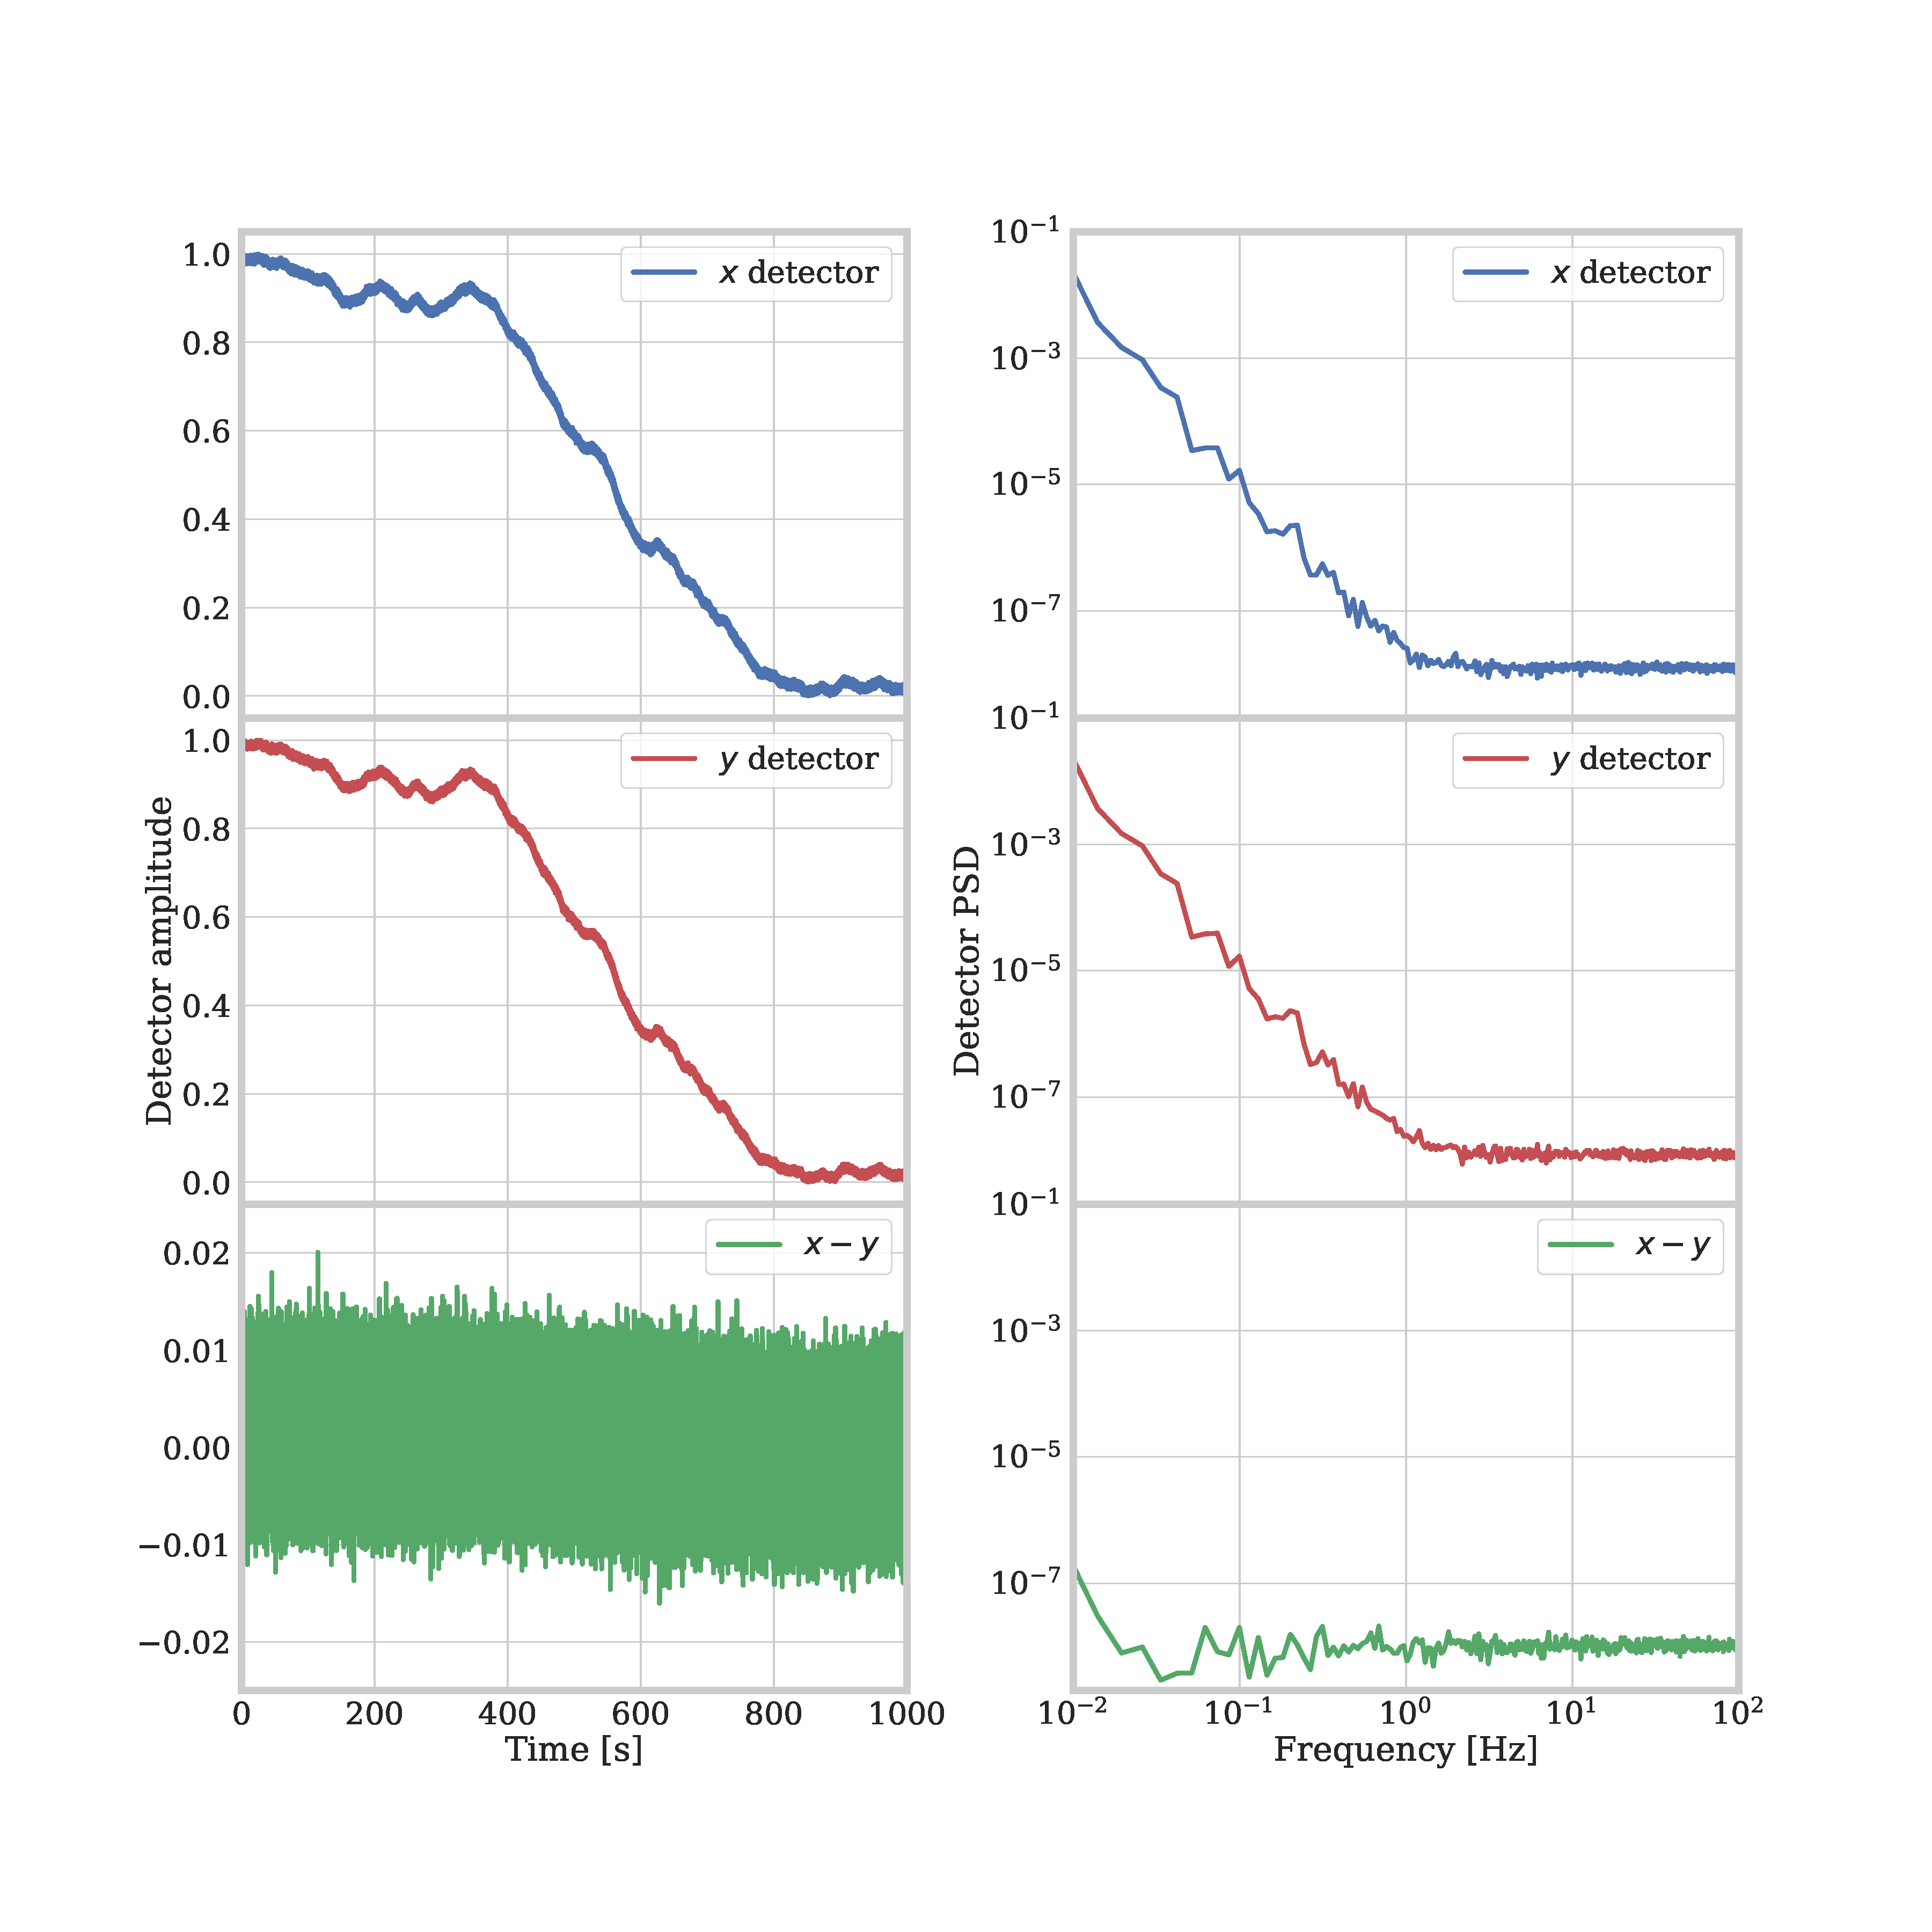
\includegraphics[width=0.8\linewidth, trim=4.5cm 5cm 5cm 5cm, clip]{PolarizationModulation/Figures/detector_differencing.pdf}
    \caption{An idealized simulation to show how detector differencing rejects unpolarized atmospheric fluctuations. The left panels show ``dummy'' time-ordered data (TOD), and the right panels show the respective power spectral densities (PSDs). In this toy simulation, the $x$ and $x$ polarimeters measure white noise, which does not correlate between the two, and atmospheric 1/f noise, which does. After the two detectors are differenced $x - y$ to extract polarization, only the white noise is left over, and the effective 1/f knee in polarization is reduced from $\sim$~1~Hz to $\lesssim$~$10^{-2}$~Hz. While the 1/f rejection is excellent in this idealized case, in practice, there are uncorrelated 1/f noise drifts between the detectors, and if that correlation is not perfectly accounted for during detector differencing, there will be residual 1/f noise that will push the $x - y$ 1/f knee higher.}
    \label{fig:detector_differencing}
\end{figure}

One increasingly popular technique to reject unpolarized atmospheric fluctuations and improve polarization sensitivity on long time scales is to employ \important{continuous polarization modulation}. The essential operating principle of a \important{polarization modulator} is to modulate the celestial polarization signal while \textit{not} modulating the intensity signal. To demonstrate this principle in its simplest form, consider a modulator operating at frequency $f_{\mathrm{mod}} = \omega_{\mathrm{mod}} / 2 \pi$, which will generate a modulating \important{detector time stream} on a single polarimeter of
\begin{eqnarray}
    d_{\mathrm{m}}(t) & = & \left< \left| E_{x}(t) \right|^{2} \right> \cos \left[ \omega_{\mathrm{mod}} t \right] + \left< \left| E_{y}(t) \right|^{2} \right> \sin \left[ \omega_{\mathrm{mod}} t \right] \nonumber \\
    & = & \left( \left< \left| E_{x}(t) \right|^{2} \right> + \left< \left| E_{y}(t) \right|^{2} \right> \right) + \left( \left< \left| E_{x}(t) \right|^{2} \right> - \left< \left| E_{y}(t) \right|^{2} \right> \right) \cos \left[ 2 \omega_{\mathrm{mod}} t \right] \nonumber \\
    & = & I(t) + Q(t) \cos \left[ 2 \omega_{\mathrm{mod}} t \right] \, ,
    \label{eq:polarization_modulation_basic}
\end{eqnarray}
where here the first term $I(t)$ is the intensity signal and the second term is the polarization signal defined in Equation~\ref{eq:detector_differencing}. This hardware-based (as opposed to analysis-based) polarization separation technique, quantified by the modulation function $\cos \left[ 2 \omega_{\mathrm{mod}} t \right]$, has several advantages over analysis-based techniques. First, a \important{single polarimeter} can measure both $x$ and $y$ polarization states, and therefore detectors do not need to be differenced to extract sky polarization. Such a technique avoids issues associated with \important{gain mismatch}, which is an umbrella term to describe when the detector outputs from two detectors don't really measure the same intensity, due to differences in bias parameters, optical properties, or responsivity (see Section~\ref{sec:simons_array_detectors} for more details about detector operation). Second, the polarization signal $\left( \left< \left| E_{x} \right|^{2} \right> - \left< \left| E_{y} \right|^{2} \right> \right)$ is modulated at frequency $f_{\mathrm{mod}}$, which is a user-defined parameter. If $f_{\mathrm{mod}}$ is large enough, then the polarization signal will be modulated faster than atmospheric fluctuations---or in other words, $ Q(t) \cos \left[ 2 \omega_{\mathrm{mod}} t \right]$ will be faster than $I(t)$---in turn improving signal-to-noise in the polarization channel.

There are many different varieties of polarization modulators that have been deployed for CMB observation, and we encourage the curious reader to review the rich modulator literature. In this dissertation, though, we instead focus on the half-wave plate (HWP) polarization modulator, which is the topic of Chapters~\ref{ch:hwp_polarization_modulation}-\ref{ch:chwp_evaluation}. HWPs are becoming increasingly popular within the CMB community, and continuously rotating HWPs have been adopted by SA and SO as principle instrumentation to enable a primordial B-mode measurement at the Atacama observation site. In the sections to follow, we overview the operating principle of a sapphire HWP for multi-chroic receivers, make explicitly how they are used to mitigate 1/f noise and beam systematics, and discuss the precedent for using HWPs in SA.

%%%%%%%%%%%%%%%%%%%%%%%%%%%%%%%%
%%%%%%%%%%%%%%%%%%%%%%%%%%%%%%%%
%%%%%%%%%%%%%%%%%%%%%%%%%%%%%%%%

\section{Atmospheric 1/f noise}
\label{sec:atmospheric_1/f_noise}

The first systematic effect that a continuously rotating HWP is designed to mitigate are those due to atmospheric fluctuations. As discussed in Section~\ref{sec:sensitivity_telescope_temperature_sky_temperature}, sky intensity is often expressed in terms of its effective temperature, and as shown in Figure~\ref{fig:so_bands_atacama}, a typical sky temperature ranges from 5~$\sim$~30~K. In contrast, as shown in Figure~\ref{fig:bb_spectrum}, the CMB primordial B-mode polarization signal is $\sim$~100~$\mathrm{n K}$, meaning that the target cosmological signal is $\sim$50 million times fainter than the sky. Even given this monumental challenge, ground-based CMB experiments are still viable competitors to balloons and satellites in the hunt for primordial B-modes because (a) the atmosphere is unpolarized, and (b) the cosmic signal is fixed, while the atmosphere varies, allowing for atmospheric noise to be averaged down.

There are a few major components to atmospheric noise. First, as discussed in Section~\ref{sec:bolocalc_site_atmosphere}, atmospheric mm-wave emission increases photon noise in the detector output. This noise is white in nature and and is largely uncorrelated between detectors on the focal plane, and the best suppression methods are to observe at a site with low PWV and oxygen content. Second, there are coordinate-dependent fluctuations in atmospheric intensity generated by spatial variations in water vapor content, such as those due to clouds. Because these variations change during the course of an observation, they are, in general, averaged down and therefore don't appear as hot and cold spots in the sky maps.\footnote{It is worth noting that ground pickup does have a fixed spatial dependence and therefore is usually handled by templates that depend on telescope coordinate} Third, and most importantly, the atmosphere varies in time, and its fluctuations follow a 1/f noise spectrum. This final effect is mitigated by the use of a polarization modulator, and therefore it is worth discussing in some detail.

According to Errard \textit{et al.}~\cite{errard_modeling_2015}, atmospheric turbulence at the Atacama site follow a Kolmogorov spectrum $\mathcal{P}_{\mathrm{atm}} \propto 1 / k^{\alpha}$, where $k$ is the three dimensional wave number and $\alpha = -11/3$. Given this atmospheric spatial structure, the detector data follows a spectrum 
$\mathcal{P}_{\mathrm{det}} \propto f^{\alpha}$~\cite{errard_modeling_2015}.\footnote{Even though this spectrum does not strictly follow a $1 / f$ shape with $\alpha = 1$, it is still referred to as \textit{1/f noise}. In other words, the term ``1/f noise'' is synonymous with low-frequency noise, which can have any value for $\alpha$.} In addition to its spectral slope, atmospheric noise is often quantified by its \important{1/f knee}, which is defined as the frequency at which 1/f noise and white noise are equal and assumes a spectrum
\begin{equation}
    N(f) = N^{\mathrm{white}} + N^{\mathrm{red}} \left( \frac{f}{f_{\mathrm{knee}}} \right)^{\alpha} \, ,
    \label{eq:1/f_knee}
\end{equation}
which is analogous to the $\ell_{\mathrm{knee}}$ Equation~\ref{eq:N_ell_low_frequency_noise}. In fact, the detector data's audio frequency $f$ can be related to angular scale $\ell$ roughly via the telescope scan speed $f_{\mathrm{scan}}$ in degrees on the sky\footnote{Note here that scan speed \textit{in sky coordinates} $f_{\mathrm{scan}}$ is related to the telescope's azimuthal rotation frequency in \textit{ground coordinates} $f_{\mathrm{tel}}$ as $f_{\mathrm{scan}} \approx f_{\mathrm{tel}} \sin[\theta_{\mathrm{El}}]$, where $\theta_{\mathrm{el}}$ is the telescope's boresight elevation. As a limiting example, if you're telescope is pointing along the z-axis (referred to as \important{zenith}), you can spin it as much as you want in $x$ and $y$, but doing so doesn't change the boresight location on the sky.} per second as
\begin{equation}
    \ell \sim \frac{f}{f_{\mathrm{scan}}} \times 180^{\circ} \, ,
    \label{eq:scan_speed_to_ell}
\end{equation}
where the $\sim$ denotes that this conversion is rough and that in practice the $N(f) \rightarrow N_{\ell}$ \important{transfer function} is a complex operation. Nonetheless, a lower $f_{\mathrm{knee}}$ in general corresponds to a lower $\ell_{\mathrm{knee}}$, which in turn corresponds to better low-$\ell$ sensitivity. Therefore, controlling atmospheric 1/f noise is central to the pursuit of primordial B-modes between $50 \lesssim \ell \gtrsim 150$. 

In addition, the characteristic length scale of Kolmogorov fluctuations is $\sim$hundreds of meters, meaning that detectors whose projection through the atmosphere is closer than this distance will see correlated noise~\cite{errard_modeling_2015}. For this reason, the degree to which atmospheric fluctuations are correlated between detectors depends both on the telescope's field of view (FOV) and on whether or not the atmosphere appears in the telescope's far field, as determined by the Fraunhofer limit
\begin{equation}
    d_{\mathrm{far}} = \frac{2 D_{\mathrm{ap}}^{2}}{\lambda} \, ,
    \label{eq:fraunhofer_far_field_limit}
\end{equation}
where $D_{\mathrm{ap}}$ is the diameter of the telescope's primary aperture, and $\lambda$ is the observed wavelength. For example, the SO SAT, which is designed with low angular resolution and therefore has a primary aperture size of $\sim$~0.5~deg, has a FOV of $\approx$~20~deg and a far-field limit of $\sim$~200~m in the 90~GHz band. In this case, the majority of atmospheric fluctuations appear in the telescope's far field and have a correlation length smaller than the FOV. Because not all detectors see the same atmospheric variations, it is possible in the SAT to \important{deproject} the atmosphere using its image on the focal plane. As a counter example, consider an SA telescope, which has an aperture size of $\approx$~2.5~m, a four-degree FOV, and a far-field limit $\sim$~4,000~m in the 90~GHz band. In this second case, a substantial fraction of atmospheric fluctuations occur in the telescope's near field, and even those which are in the far field are correlated over regions larger than the telescope's FOV. Because atmospheric fluctuations are highly correlated across the full focal plane, they are said to be \important{common-mode fluctuations}. Removing such correlated signals from all detectors dramatically reduces an SA telescope's sensitivity to large-angular-scale CMB signals, and for this reason, among others, it is critically important to suppress the impact of common-mode atmospheric fluctuations in order to enable low-$\ell$ science on SA style telescopes.

%%%%%%%%%%%%%%%%%%%%%%%%%%%%%%%%
%%%%%%%%%%%%%%%%%%%%%%%%%%%%%%%%
%%%%%%%%%%%%%%%%%%%%%%%%%%%%%%%%

\section{Polarized beam systematics}
\label{sec:polarized_beam_systematics}

The second systematic effect mitigated by a HWP is I-to-P leakage caused either by non-idealities in the telescope optics or by differential optical response between two orthogonal polarimeters on the same detector pixel. These inadvertent conversions from intensity to polarization pose several challenges during data analysis, including CMB temperature fluctuations bleeding into polarization and residual atmospheric 1/f noise even after detector differencing (see Section~\ref{sec:atmospheric_1/f_noise}). These beam systematics are typically described in terms of their monopole, dipole, and quadrupole moments, as shown in Figure~blah.

\begin{figure}[!t]
    \centering
    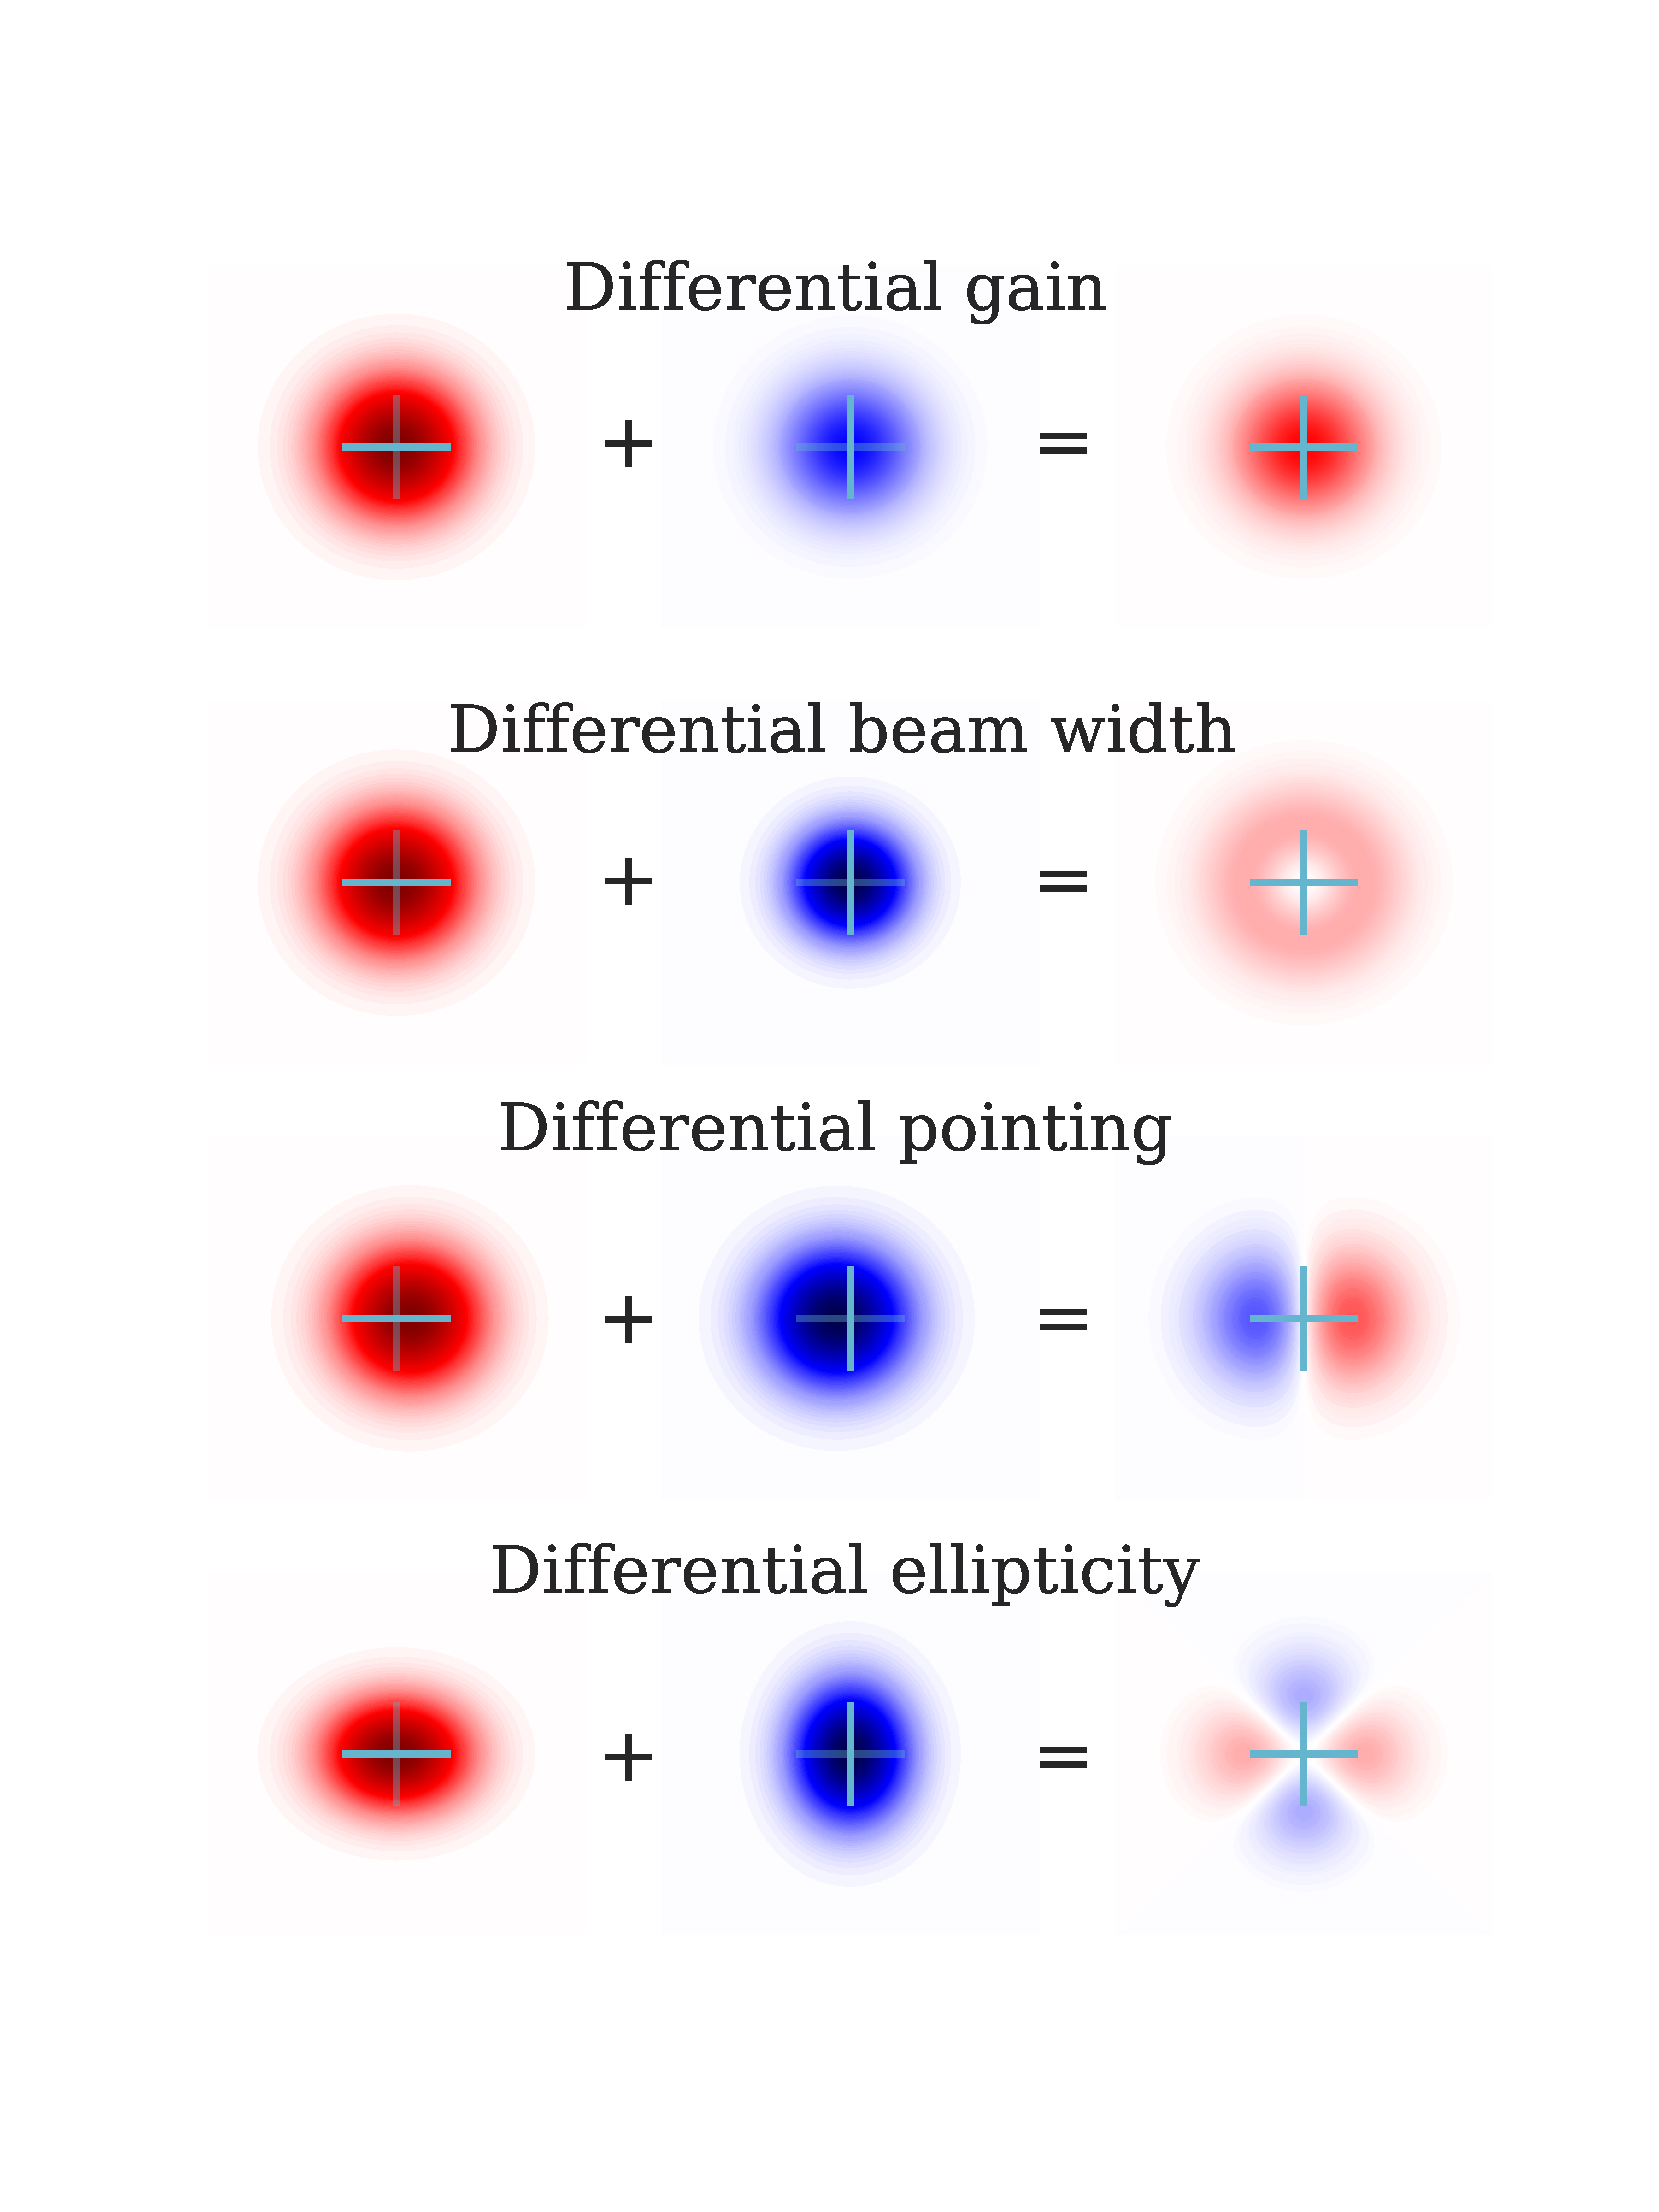
\includegraphics[width=0.7\linewidth, trim=9.5cm 11cm 7.5cm 9cm, clip]{PolarizationModulation/Figures/beam_systematics.pdf}
    \caption{Differential beam systematics}
    \label{fig:beam_systematics}
\end{figure}

Monopole systematics arise due to either \important{differential gain} or \important{differential beam width} that when differenced give rise to a rotationally symmetric residual. Dipole systematics arise from \important{differential pointing}, which is the effect of the two detectors not being fully co-located on the sky. Quadrupole systematics arise from \important{differential ellipticity}\footnote{Quadrupolar effects can also arise from some combination of differential gain/beam width and differential pointing, but the resulting effect is practically identical to that of differential ellipticity, and so we choose not to discuss such higher-order combinations of effects.}, which is the effect of the two detectors having different beam \textit{shapes}, specifically having ellipticities whose major ellipse axes do not align. While monopole and dipole beam systematics can be removed by taking accurate beam maps and using them during analysis, the quadrupolar term is difficult to distinguish from the polarization signal itself, placing a huge importance on beam symmetry during instrument design and evaluation.

%%%%%%%%%%%%%%%%%%%%%%%%%%%%%%%%
%%%%%%%%%%%%%%%%%%%%%%%%%%%%%%%%
%%%%%%%%%%%%%%%%%%%%%%%%%%%%%%%%

\section{Sapphire achromatic HWP}
\label{sec:sapphire_achromatic_hwp}

Continuous HWP polarization modulation is a powerful tool to mitigate atmospheric 1/f noise and beam systematics. A detailed discussion of the HWP's workings are in the subsections to follow, but at its most basic level, a continuous HWP spins the sky polarization signal at a well-monitored frequency, which in turn modulates the signal on each polarimeter. This operation applies a time-dependent global rotation to the sky polarization signal, which in turn allows both polarimeters to measure each polarization state, and because the HWP does not---to leading order---modulate the intensity signal, the HWP eliminates the need for detector differencing to extract the incident polarization signal. In addition, if this continuous rotation is fast enough, the HWP up-converts to the sky polarization signal to temporal frequencies larger than those of the atmospheric /1f noise, therefore dramatically suppressing turbulence-induced, long-time-scale residuals in the demodulated detector data. 

In this section, we review the basics of HWP polarization modulation and discuss its applications to a sapphire achromatic HWP. Then, later in the chapter, we discuss the impact of HWP modulators on the CMB field and how these impacts are being leveraged by SA and SO.

%%%%%%%%%%%%%%%%%%%%%%%%%%%%%%%%
%%%%%%%%%%%%%%%%%%%%%%%%%%%%%%%%

\subsection{Stokes polarization}
\label{sec:stokes_polarization}

Polarization is often decomposed into one of two bases. The first, and perhaps most familiar to physicists, are Jones vectors. A Jones basis consists of two orthogonal basis vectors $(\hat{r}_{1}, \hat{r}_{2})$ and is used to describe fully polarized light propagating along the $\vec{r}_{3}$ direction
\begin{equation}
    \begin{pmatrix}
    E_{1}(t) \\
    E_{2}(t) \\
    0
    \end{pmatrix}
    =
    \begin{pmatrix}
    E_{0, 1} e^{i \phi_{1}} \\
    E_{0, 2} e^{i \phi_{2}} \\
    0
    \end{pmatrix}
    e^{i ( k r_{3} - \omega t)}\, ,
    \label{eq:jones_matrix_definition}
\end{equation}
where $E_{0, 1}$ and $E_{0, 2}$ are the wave amplitudes and where phase factors. In this basis, the polarization can be manipulated by a collection of \important{Jones matrices} which are used to both rotate linear polarization and convert to and from linear to circular polarization. The subset of these operations that will be most useful for our purposes are
\begin{eqnarray}
    \begin{pmatrix}
    E_{x} \\
    0 \\
    0
    \end{pmatrix}
    =
    \vec{E}
    \begin{pmatrix}
    1 & 0 \\
    0 & 0
    \end{pmatrix}
    \; \; & ; & \; \;
    \begin{pmatrix}
    0 \\
    E_{y} \\
    0
    \end{pmatrix}
    =
    \vec{E}
    \begin{pmatrix}
    0 & 0 \\
    0 & 1
    \end{pmatrix}
    \nonumber \\ % Newline
    \begin{pmatrix}
    E_{a} \\
    0 \\
    0
    \end{pmatrix}
    =
    \vec{E}
    \begin{pmatrix}
    1/2 & 1/2 \\
    1/2 & 1/2
    \end{pmatrix}
    \; \; & ; & \; \;
    \begin{pmatrix}
    0 \\
    E_{b} \\
    0
    \end{pmatrix}
    =
    \vec{E}
    \begin{pmatrix}
    1/2 & -1/2 \\
    -1/2 & 1/2
    \end{pmatrix}
    \label{eq:jones_matrices}
    \\ % Newline
    \begin{pmatrix}
    E_{l} \\
    0 \\
    0
    \end{pmatrix}
    =
    \vec{E}
    \begin{pmatrix}
    1/2 & -i/2 \\
    i/2 & 1/2
    \end{pmatrix}
    \; \; & ; & \; \;
    \begin{pmatrix}
    0 \\
    E_{r} \\
    0
    \end{pmatrix}
    =
    \vec{E}
    \begin{pmatrix}
    1/2 & i/2 \\
    -i/2 & 1/2
    \end{pmatrix} \nonumber \, ,
\end{eqnarray}
where here $\vec{E}$ is 100\% polarized in the $(\hat{x}, \hat{y})$ basis. These three Jones bases are shown in Figure~blah.

\begin{figure}[!t]
    \centering
    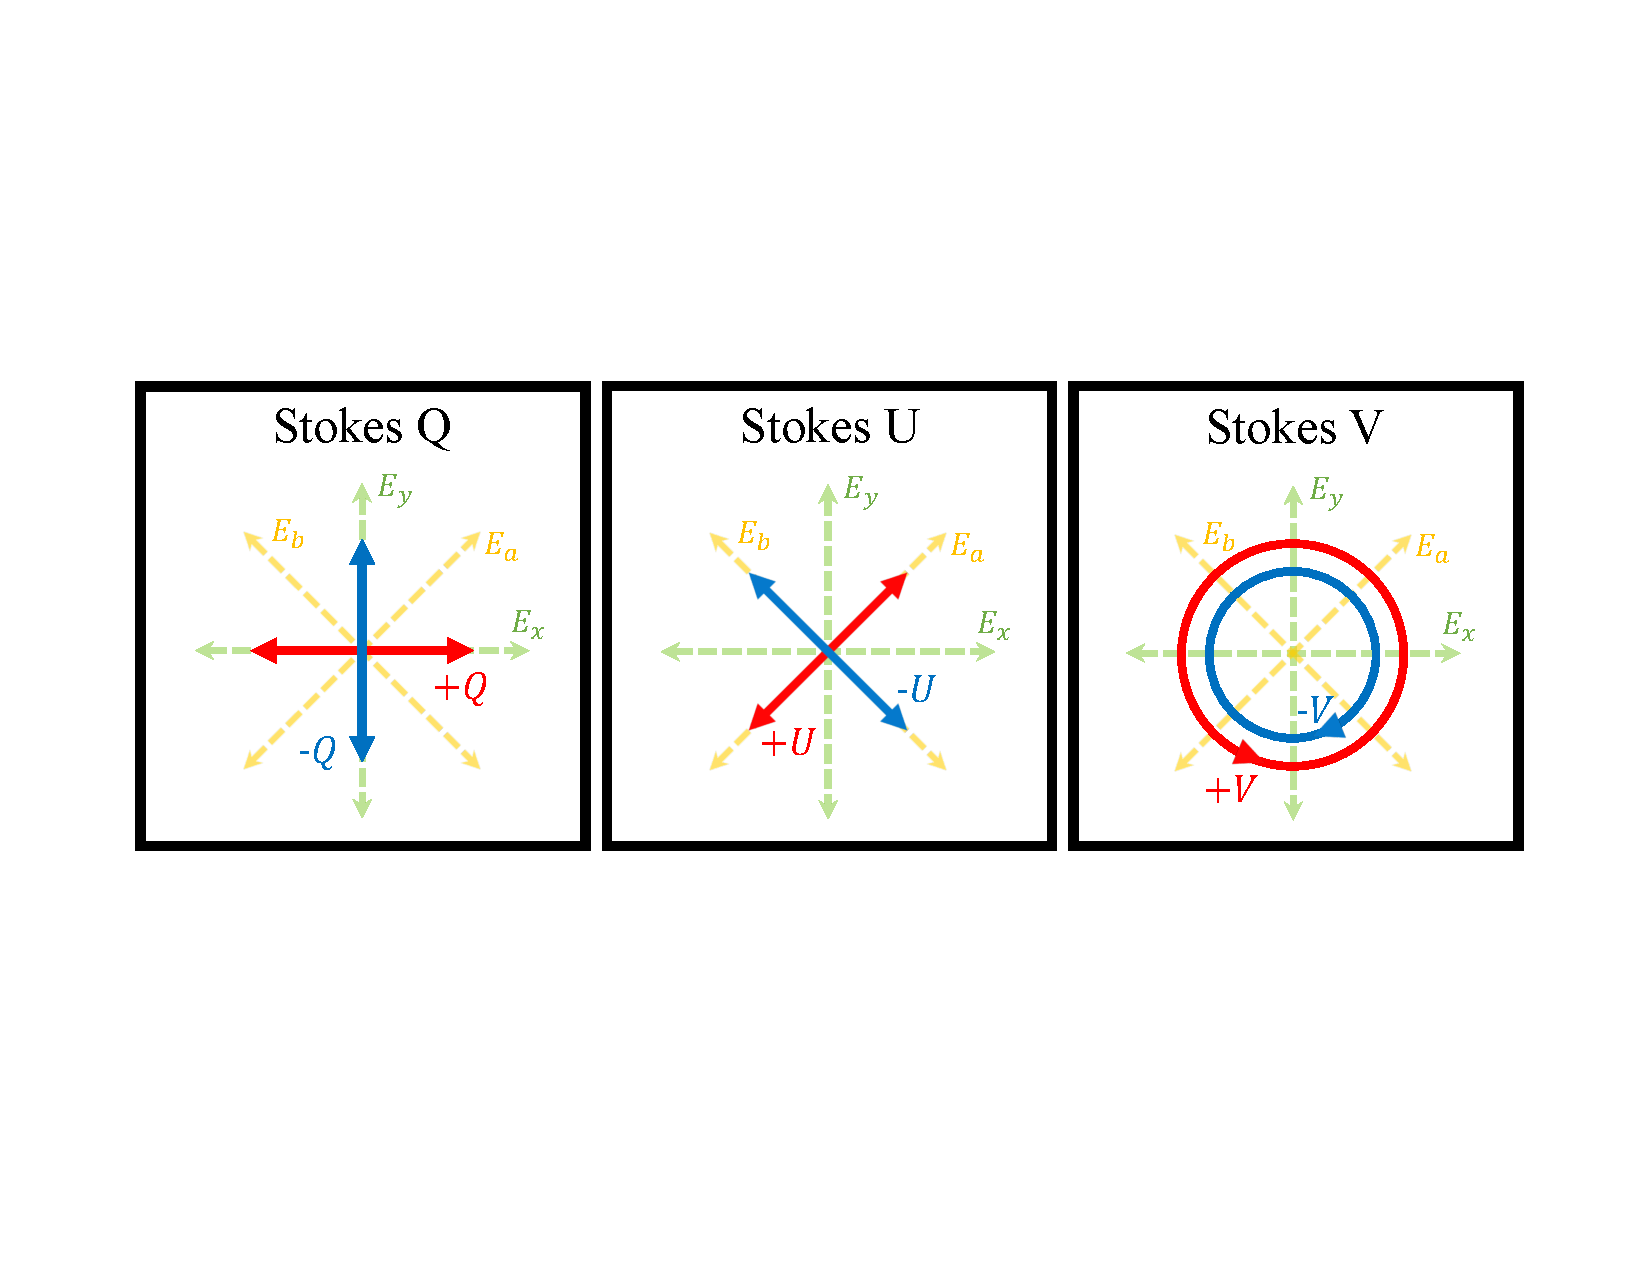
\includegraphics[width=\linewidth, trim=2cm 7cm 2cm 6cm, clip]{PolarizationModulation/Figures/stokes_parameters.pdf}
    \caption{Relationship between the Jones vectors and Stokes vectors. Linear polarimeters, such as those used to measure CMB polarization, are sensitive to Q and U but not V.}
    \label{fig:stokes_parameters}
\end{figure}

While Jones vectors are a familiar, simple description of \textit{fully} polarized light, the sources that astronomical experiments observe are only partially polarized, and there for the bases in Equation~\ref{eq:jones_matrices} are inconvenient to describe CMB polarimetry. Therefore, we introduce the \important{Stokes parameters}, which can be written in terms of the Jones vectors as
\begin{equation}
    \begin{array}{r@{}l}
    I &{}\equiv \left< \left| E_{x} \right|^{2} \right> + \left< \left| E_{y} \right|^{2} \right> \\
    Q &{}\equiv  \left< \left| E_{x} \right|^{2} \right> - \left< \left| E_{y} \right|^{2} \right> \\
    U &{}\equiv  \left< \left| E_{a} \right|^{2} \right> - \left< \left| E_{b} \right|^{2} \right> \\
    V &{}\equiv  \left< \left| E_{r} \right|^{2} \right> - \left< \left| E_{l} \right|^{2} \right> \, .
    \end{array}
    \label{eq:stokes_parameters}
\end{equation}
The Stokes representation of polarization has several advantages over that of the Cartesian representation for CMB measurements. First of all, they are written in terms of intensity $\left| E_{i} \right|^{2}$, which is useful for bolometers that detect power instead of amplitude and phase. Second, the Stokes vectors are inherently statistical and are a measure of the expectation value of the square field amplitude, denoted by the angle brackets $\left< \cdot \right>$. This characteristic is also useful for CMB mappers whose goal is to make many measurements of a given sky patch/source, average down the noise, and better constrain the expectation value of the polarization properties across the sky. Third, the Stokes parameters naturally handle partial polarization, and the polarization fraction is defined as
\begin{equation}
    P \equiv \frac{\sqrt{Q^{2} + U^{2} + V^{2}}}{I} \, .
    \label{eq:stokes_polarization_fraction}
\end{equation}
Finally, the Stokes decomposition is natural for extracting polarization via the differencing of orthogonal detectors, which is a common technique used in CMB experiments (more on this below). Relating back to Equation~\ref{eq:emodes_bmodes}, E-modes and B-modes are also nicely described in the basis of Stokes vectors, and for this reason, making $Q$ and $U$ maps of CMB polarization are a necessary analysis step on the path towards E-mode and B-mode maps.

While the math of polarization modulators can be equivalently described in either the Jones or Stokes bases, from now on, for the reasons laid out above, we work in the Stokes basis.

%%%%%%%%%%%%%%%%%%%%%%%%%%%%%%%%
%%%%%%%%%%%%%%%%%%%%%%%%%%%%%%%%

\subsection{Birefringent HWP}
\label{sec:birefringent_hwp}

A half-wave plate is a birefringent medium whose geometry is tuned to introduce a phase shift of $\pi$ between light along the medium's two birefringent axes. The dielectric tensor of such a birefringent material can be written as
\begin{equation}
    \varepsilon_{i j} = 
    \begin{pmatrix}
    \varepsilon_{\mathrm{e}} & 0 & 0 \\
    0 & \varepsilon_{\mathrm{o}} & 0 \\
    0 & 0 & \varepsilon_{\mathrm{o}} \\
    \end{pmatrix} \, ,
\end{equation}
where $\varepsilon_{\mathrm{e}}$ is medium's dielectric constant along the \important{extraordinary} axis and where $\varepsilon_{\mathrm{o}}$ is its dielectric constant along its \important{ordinary axes}. 

When an electromagnetic wave described by vector $\vec{E} = E_{0} \hat{k}$ enters the dielectric medium, it can be decomposed into an ordinary and extraordinary wave as
\begin{equation}
    \begin{array}{r@{}l}
    \vec{E}_{1} &{}= E_{1} \hat{e}_{1} \; ; \; \hat{e}_{1} \propto \left( 0, k_{z}, -k_{y} \right) \\
    \vec{E}_{2} &{}= E_{2} \hat{e}_{2} \; ; \; \hat{e}_{2} \propto \left( 1 - k_{x}^{2}, -k_{x} k_{y}, -k_{x} k_{z} \right) \, .
    \end{array}
    \label{eq:ordinary_extraordinary_waves}
\end{equation}
The phase velocities (or the velocity at which the wave propagates through the medium) of the ordinary and extraordinary waves are
\begin{equation}
    \begin{array}{r@{}l}
    v_{1} &{}= v_{o} \\
    v_{2} &{}= \sqrt{v_{e}^{2} \left( 1 - k_{x}^{2} \right) + v_{o}^{2} k_{x}^{2}} \, ,
    \end{array}
    \label{eq:ordinary_extraordinary_wave_velocities}
\end{equation}
where
\begin{equation}
    \begin{array}{r@{}l}
    v_{o} &{}\equiv \frac{c}{n_{o}} \\
    v_{e} &{}\equiv \frac{c}{n_{e}} \, ,
    \end{array}
    \label{eq:ordinary_extraordinary_axes_velocities}
\end{equation}
In the limit of normal incidence $\hat{k} = (0, 0, k_{z})$, $v_{2} = v_{e}$, and the basis vectors for the ordinary and extraordinary waves defined in Equation~\ref{eq:ordinary_extraordinary_waves} coincides with the ordinary and extraordinary axes of the birefringent medium $(\vec{e}_{1}, \vec{e}_{2}) = (\hat{\varepsilon}_{e}, \hat{\varepsilon}_{o})$.

\begin{figure}
    \centering
    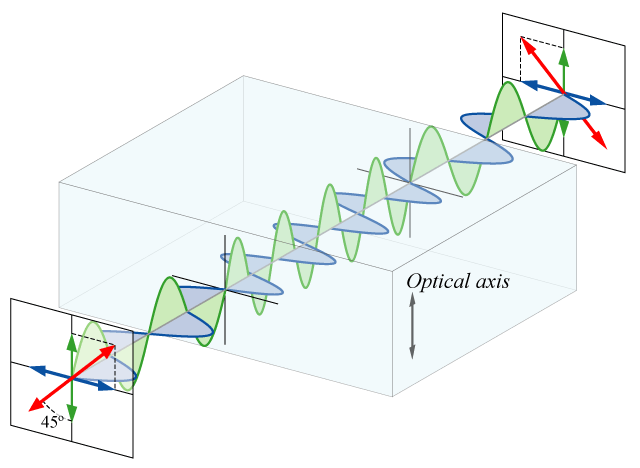
\includegraphics[width=0.7\linewidth]{PolarizationModulation/Figures/Waveplate.png}
    \caption[Depiction of how a half-wave plate manipulates polarization orientation]{A half-wave plate is a birefringent medium whose thickness is tuned to introduce a 180 degree phase shift between the crystal-axis components of a linearly polarized input electric field. This phase shift rotates the polarization direction, mirroring it over the crystal's optical axis. This figure shows a perfect waveplate, which can only be achieved for a single wavelength, making a single-plate waveplate a narrow-band instrument \cite{noauthor_waveplate_2019}.}
    \label{fig:halfwave_plate_cartoon}
\end{figure}

A half-wave plate is a birefringent material whose thickness is tuned to generate a $\pi$ phase delay between light polarized along its ordinary and extraordinary axes. Assume that the birefringent dielectric is cut like shown in Figure~blah, such that $(\hat{\varepsilon}_{e}, \hat{\varepsilon}_{o})$ lie in the plane of the surface. If the plate has a thickness $d$, then the phase delay generated between the ordinary and extraordinary waves is
\begin{equation}
    \delta \phi = 2 \pi \left( \frac{d}{v_{e} / \nu} - \frac{d}{v_{o} / \nu} \right) = \frac{2 \pi \left( n_{e} - n_{o} \right) d}{\lambda} \, .
    \label{eq:birefringent_phase_delay}
\end{equation}
where $\lambda$ is the wavelength of the incident light in a vacuum. For a half-wave plate, $\delta \phi = \pi$, which gives the thickness of an ideal HWP to be
\begin{equation}
    d_{\mathrm{HWP}} = \frac{\lambda}{2 \left( n_{e} - n_{o} \right)} \, .
    \label{eq:hwp_ideal_thickness}
\end{equation}
Note that a HWP can only be ideal at a single frequency, and therefore when linearly polarized incident light has a wavelength $\neq \lambda$, the HWP doesn't perfectly preserve its linear polarization.

%%%%%%%%%%%%%%%%%%%%%%%%%%%%%%%%
%%%%%%%%%%%%%%%%%%%%%%%%%%%%%%%%

\subsection{Muller matrices}
\label{sec:muller_matrix_formalism}

In order to apply the phase-delay discussion in Section~\ref{sec:birefringent_hwp} to the Stokes parameters, we need to utilize the machinery of \important{Mueller matrices}, which are 4x4 matrix operators that act on the \important{Stokes} vector $\vec{S} = (I, Q, U, V)$. We can express the Mueller matrix operation as
\begin{equation}
    \vec{S}_{\mathrm{out}} = M \vec{S}_{\mathrm{in}} \, ,
    \label{eq:mueller_matrix_operation}
\end{equation}
where $\vec{S}_{\mathrm{in}}$ and $\vec{s}_{\mathrm{out}}$ are the input and output Stokes vectors, respectively. As shown in Figure~blah, a perfect HWP ``fips'' the input polarization with respect to its extraordinary axis. In terms of the Stokes parameters, this behavior is equivalent to inverting the Q polarization component to -Q (and V polarization to -V)
\begin{equation}
    M_{\mathrm{HWP}}^{\mathrm{ideal}}
    =
    \begin{pmatrix}
    1 & 0 & 0 & 0 \\
    0 & 1 & 0 & 0 \\
    0 & 0 & -1 & 0 \\
    0 & 0 & 0 & -1 \\
    \end{pmatrix} \, ,
    \label{eq:mueller_matrix_ideal_hwp}
\end{equation}
where here the extraordinary axis is assumed to be either vertical or horizontal. 

As mentioned earlier, a HWP made from a birefringent substrate is only perfect for a single input frequency: at frequencies increasingly far from $\lambda_{\mathrm{HWP}}$, the incident light is increasingly converted to elliptical polarization (or, equivalently, a mixture of linear and circular polarization). In order to calculate this effect, we introduce a more generalized Mueller matrix formalism for the HWP system. 

Consider an input Stokes vector
\begin{equation}
    \vec{S}_{\mathrm{in}}
    =
    I(\nu) 
    \begin{pmatrix}
    1 \\
    P_{\mathrm{in}} \cos 2 \alpha_{\mathrm{in}} \\ P_{\mathrm{in}} \sin 2 \alpha_{\mathrm{in}} \\
    0
    \end{pmatrix}
    \label{eq:mueller_matrix_Sin}
\end{equation}
where $I(\nu)$ is the intensity as a function of microwave frequency $\nu$, $P_{\mathrm{in}} = \sqrt{Q^{2} + U^{2}} / I$ is the input linear polarization fraction, and $\alpha_{\mathrm{in}}$ is the angle between the input polarization vector and a fixed coordinate system. Note that Stokes parameters are sometimes called a \important{spin-2 field} because they are symmetric under a $\pi / 2$ rotation. The effect of the HWP is to introduce a phase delay between the birefringent axes via the operation
\begin{equation}
    \vec{S}_{\mathrm{out}} = R(- \rho) \Gamma ( \delta) R(\rho) \vec{S}_{\mathrm{in}} \, ,
    \label{eq:single_hwp_mueller_matrix_operation}
\end{equation}
where $\delta$ is the phase delay defined in Equation~\ref{eq:birefringent_phase_delay}. The first and final operators on $S_{\mathrm{in}}$ are rotation matrices
\begin{equation}
    R(\Psi)
    =
    \begin{pmatrix}
    1 & 0 & 0 & 0 \\
    0 & \cos 2 \Psi & - \sin 2 \Psi & 0 \\
    0 & - \sin 2 \Psi & \cos 2 \Psi & 0 \\
    0 & 0 & 0 & 1 \\
    \end{pmatrix} \, ,
    \label{eq:rotation_mueller_matrix}
\end{equation}
and are used to rotate the Stokes vector into and out of the dielectric coordinate system $\hat{\varepsilon}_{i} = (\hat{\varepsilon}_{e}, \hat{\varepsilon}_{o}, \hat{\varepsilon}_{o})$. Once in the frame of the ordinary and extraordinary axes, the phase delay operator modifies the Stokes vector
\begin{equation}
    \Gamma(\delta)
    =
    \begin{pmatrix}
    1 & 0 & 0 & 0 \\
    0 & 1 & 0 & 0 \\
    0 & 0 & \cos \delta & -\sin \delta \\
    0 & 0 & \sin \delta & \cos \delta \\
    \end{pmatrix} \, ,
    \label{eq:mueller_phase_delay_matrix}
\end{equation}
which reduces to the idealized matrix in Equation~\ref{eq:mueller_matrix_ideal_hwp} when $\delta = \pi$.

%%%%%%%%%%%%%%%%%%%%%%%%%%%%%%%%
%%%%%%%%%%%%%%%%%%%%%%%%%%%%%%%%

\subsection{Achromatic HWP}
\label{sec:achromatic_hwp}

\begin{figure}[!t]
    \centering
    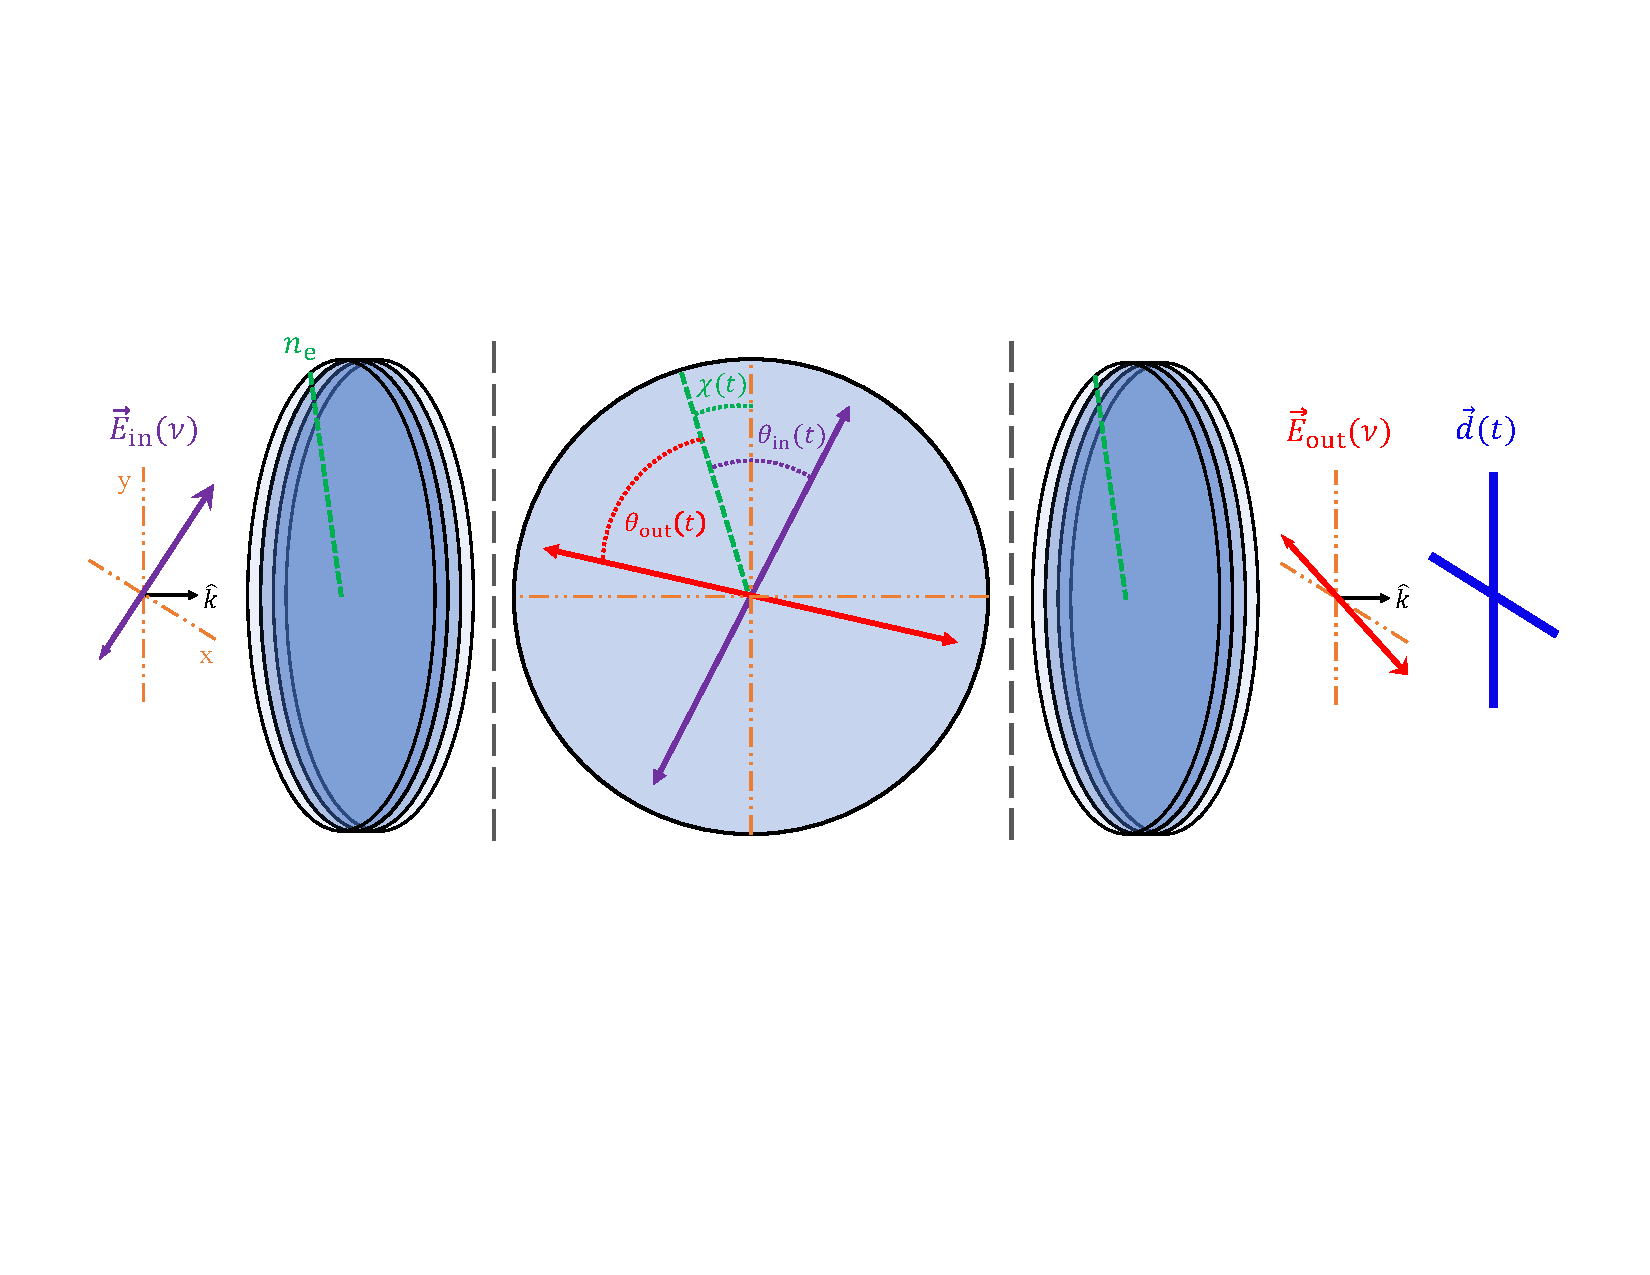
\includegraphics[width=\linewidth, trim=1.2cm 7cm 1.2cm 4cm, clip]{PolarizationModulation/Figures/HWP_cartoon.pdf}
    \caption{A cartoon of the sapphire achromatic HWP. Linearly polarized input light, with wave vector $\hat{k}$ and field vector $\vec{E}_{\mathrm{in}}(\nu)$, is rotated by twice its polarization angle $\theta_{\mathrm{in}}(t)$ with respect to the HWP axis---which coincides with the first sapphire piece's extraordinary crystal axis $n_{\mathrm{e}}$---plus a frequency-dependent phase $2 \phi(\nu)$. A continuously rotating HWP spins at a constant velocity $\mathrm{d} \chi / \mathrm{d} t = 2 \pi f_{\mathrm{HWP}}$, modulating the output field vector $E_{\mathrm{out}}(t)$ at $2 f_{\mathrm{HWP}}$ and the detected polarimeter power $\vec{d}(t)$ at $4 f_{\mathrm{HWP}}$.}
    \label{fig:ahwp_cartoon}
\end{figure}

As noted by Equation~\ref{eq:hwp_ideal_thickness}, a HWP of ``ideal'' thickness is only ideal for a single frequency, and as bandwidth increases, so too does the HWP's conversion of linear polarization into elliptical polarization. Since the CMB has no measurable circular polarization\footnote{There are theories of \textit{cosmological birefringence} that predict some amount of cosmic circular polarization, but these have not been measured or validated}, and because linear polarimeters are not capable of measuring circular polarization, this conversion from linear to elliptical polarization gives rise to a \important{polarization efficiency loss}, which is typically quantified by the HWP's \important{linear polarization modulation efficiency}
\begin{equation}
    \varepsilon_{\mathrm{mod}} = \frac{P_{\mathrm{out}}}{P_{\mathrm{in}}} \, ,
    \label{eq:linear_polarization_modulation_efficiency}
\end{equation}
where $P_{\mathrm{out}}$ is the output linear polarization fraction.

\begin{figure}[!t]
    \centering
    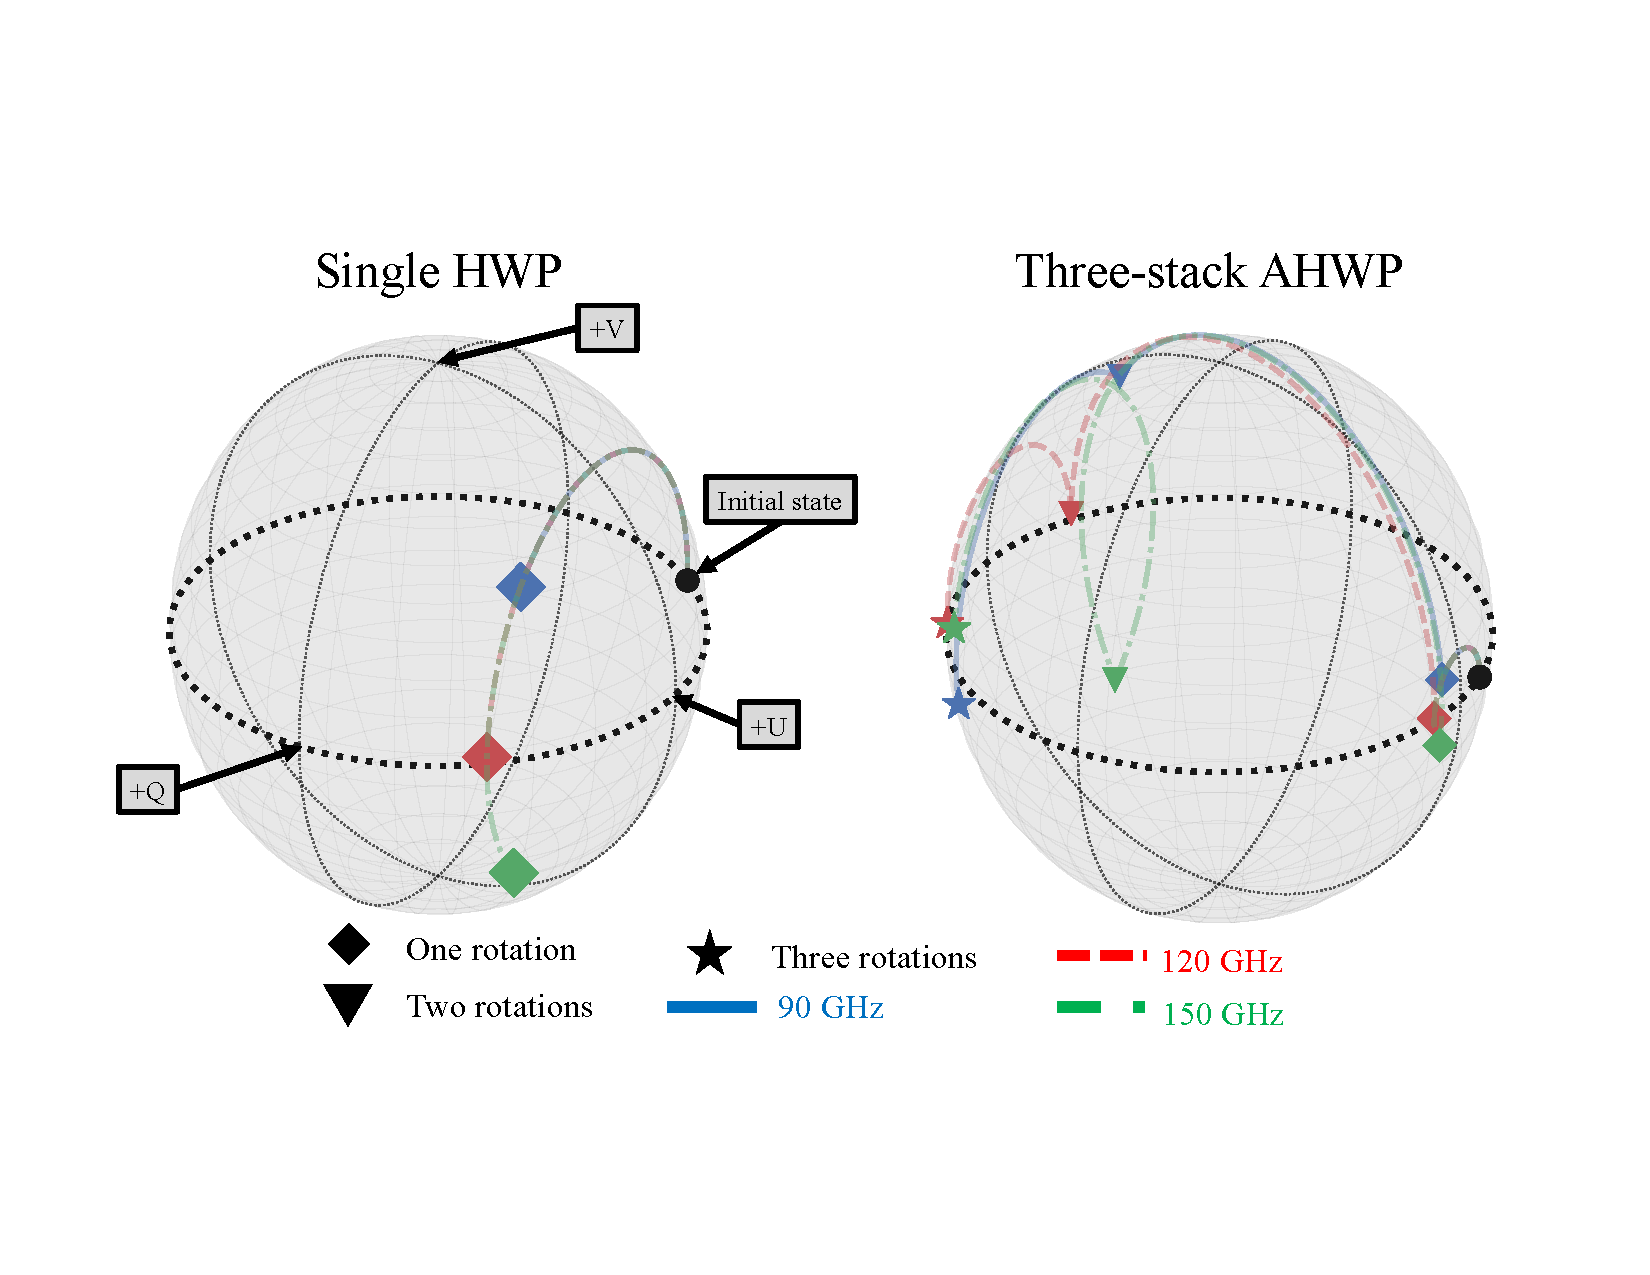
\includegraphics[width=\linewidth, trim=2cm 4cm 2cm 4cm, clip]{PolarizationModulation/Figures/poincare_sphere.pdf}
    \caption{Poincare sphere}
    \label{fig:poincare_sphere}
\end{figure}

One popular method to achieve broadband polarization modulation efficiency is to use an \important{achromatic HWP} (AHWP), or one that is less particular about the ``color'' of the incident light. There are many ways to achieve a broad bandwidth, including using engineered capacitive grids or metamaterial layers, but one particularly common solution, which SA and SO use, is to employ a Pancharatnam AHWP. The basic concept of a \important{Pancharatnam stack} is to increase the number of degrees of freedom that can be used to manipulate how the HWP transfers $\vec{S}_{\mathrm{in}}$ to $\vec{S}_{\mathrm{out}}$\footnote{This general concept is similar in spirit to that which is used to increase the bandwidth of anti-reflection coatings, a topic that we cover in detail in Chapter~blah} by increasing the number of birefringent plates that compose the HWP stack. Adding more plates modifies Equation~\ref{eq:single_hwp_mueller_matrix_operation} to become
\begin{equation}
    \vec{S}_{\mathrm{out}} = \prod_{i = 0}^{m} \left[ R(- \rho - \theta_{i}) \Gamma (\delta) R(\rho + \theta_{i}) \right] \vec{S}_{\mathrm{in}} \, ,
    \label{eq:ahwp_mueller_matrix_operation}
\end{equation}
where here $\theta_{i}$ is the orientation of each plate in the stack of $m$. The ordering of the product is from the sky towards the detector, or in other words, in the order in which the plates operate on the polarization.

An AHWP can be composed of a stack of any birefringent plates, but an appealing material selection for mm-wave observation is sapphire, which both is highly transparent at $\sim$~100~GHz with $\tan \delta \sim 10^{-4}$ (see Equation~\ref{eq:loss_tangent} for a discussion of dielectric loss) and has a large differential index $(n_{e} - n_{o}) \approx (3.4 - 3.05) \approx 0.35$, which in turn minimizes its thickness $d_{\mathrm{HWP}} \sim 3.5$~mm. For these reasons and others discussed in Section~blah, SA and SO use sapphire AHWPs as polarization modulators.

%%%%%%%%%%%%%%%%%%%%%%%%%%%%%%%%
%%%%%%%%%%%%%%%%%%%%%%%%%%%%%%%%
%%%%%%%%%%%%%%%%%%%%%%%%%%%%%%%%

\section{AHWP performance}
\label{sec:ahwp_performance}

Armed with the formalism for AHWPs given by Equation~\ref{eq:ahwp_mueller_matrix_operation}, we are now in a position to evaluate the performance of an AHWP for SA and SO. For the purposes of keeping the discussion focused, we will only inspect the MF cameras, which observe at 90 and 150~GHz, noting that much of this investigations transfers relatively trivially to the 34/40~GHz and 220/270~GHz cameras. 

\begin{figure}[!t]
    \centering
    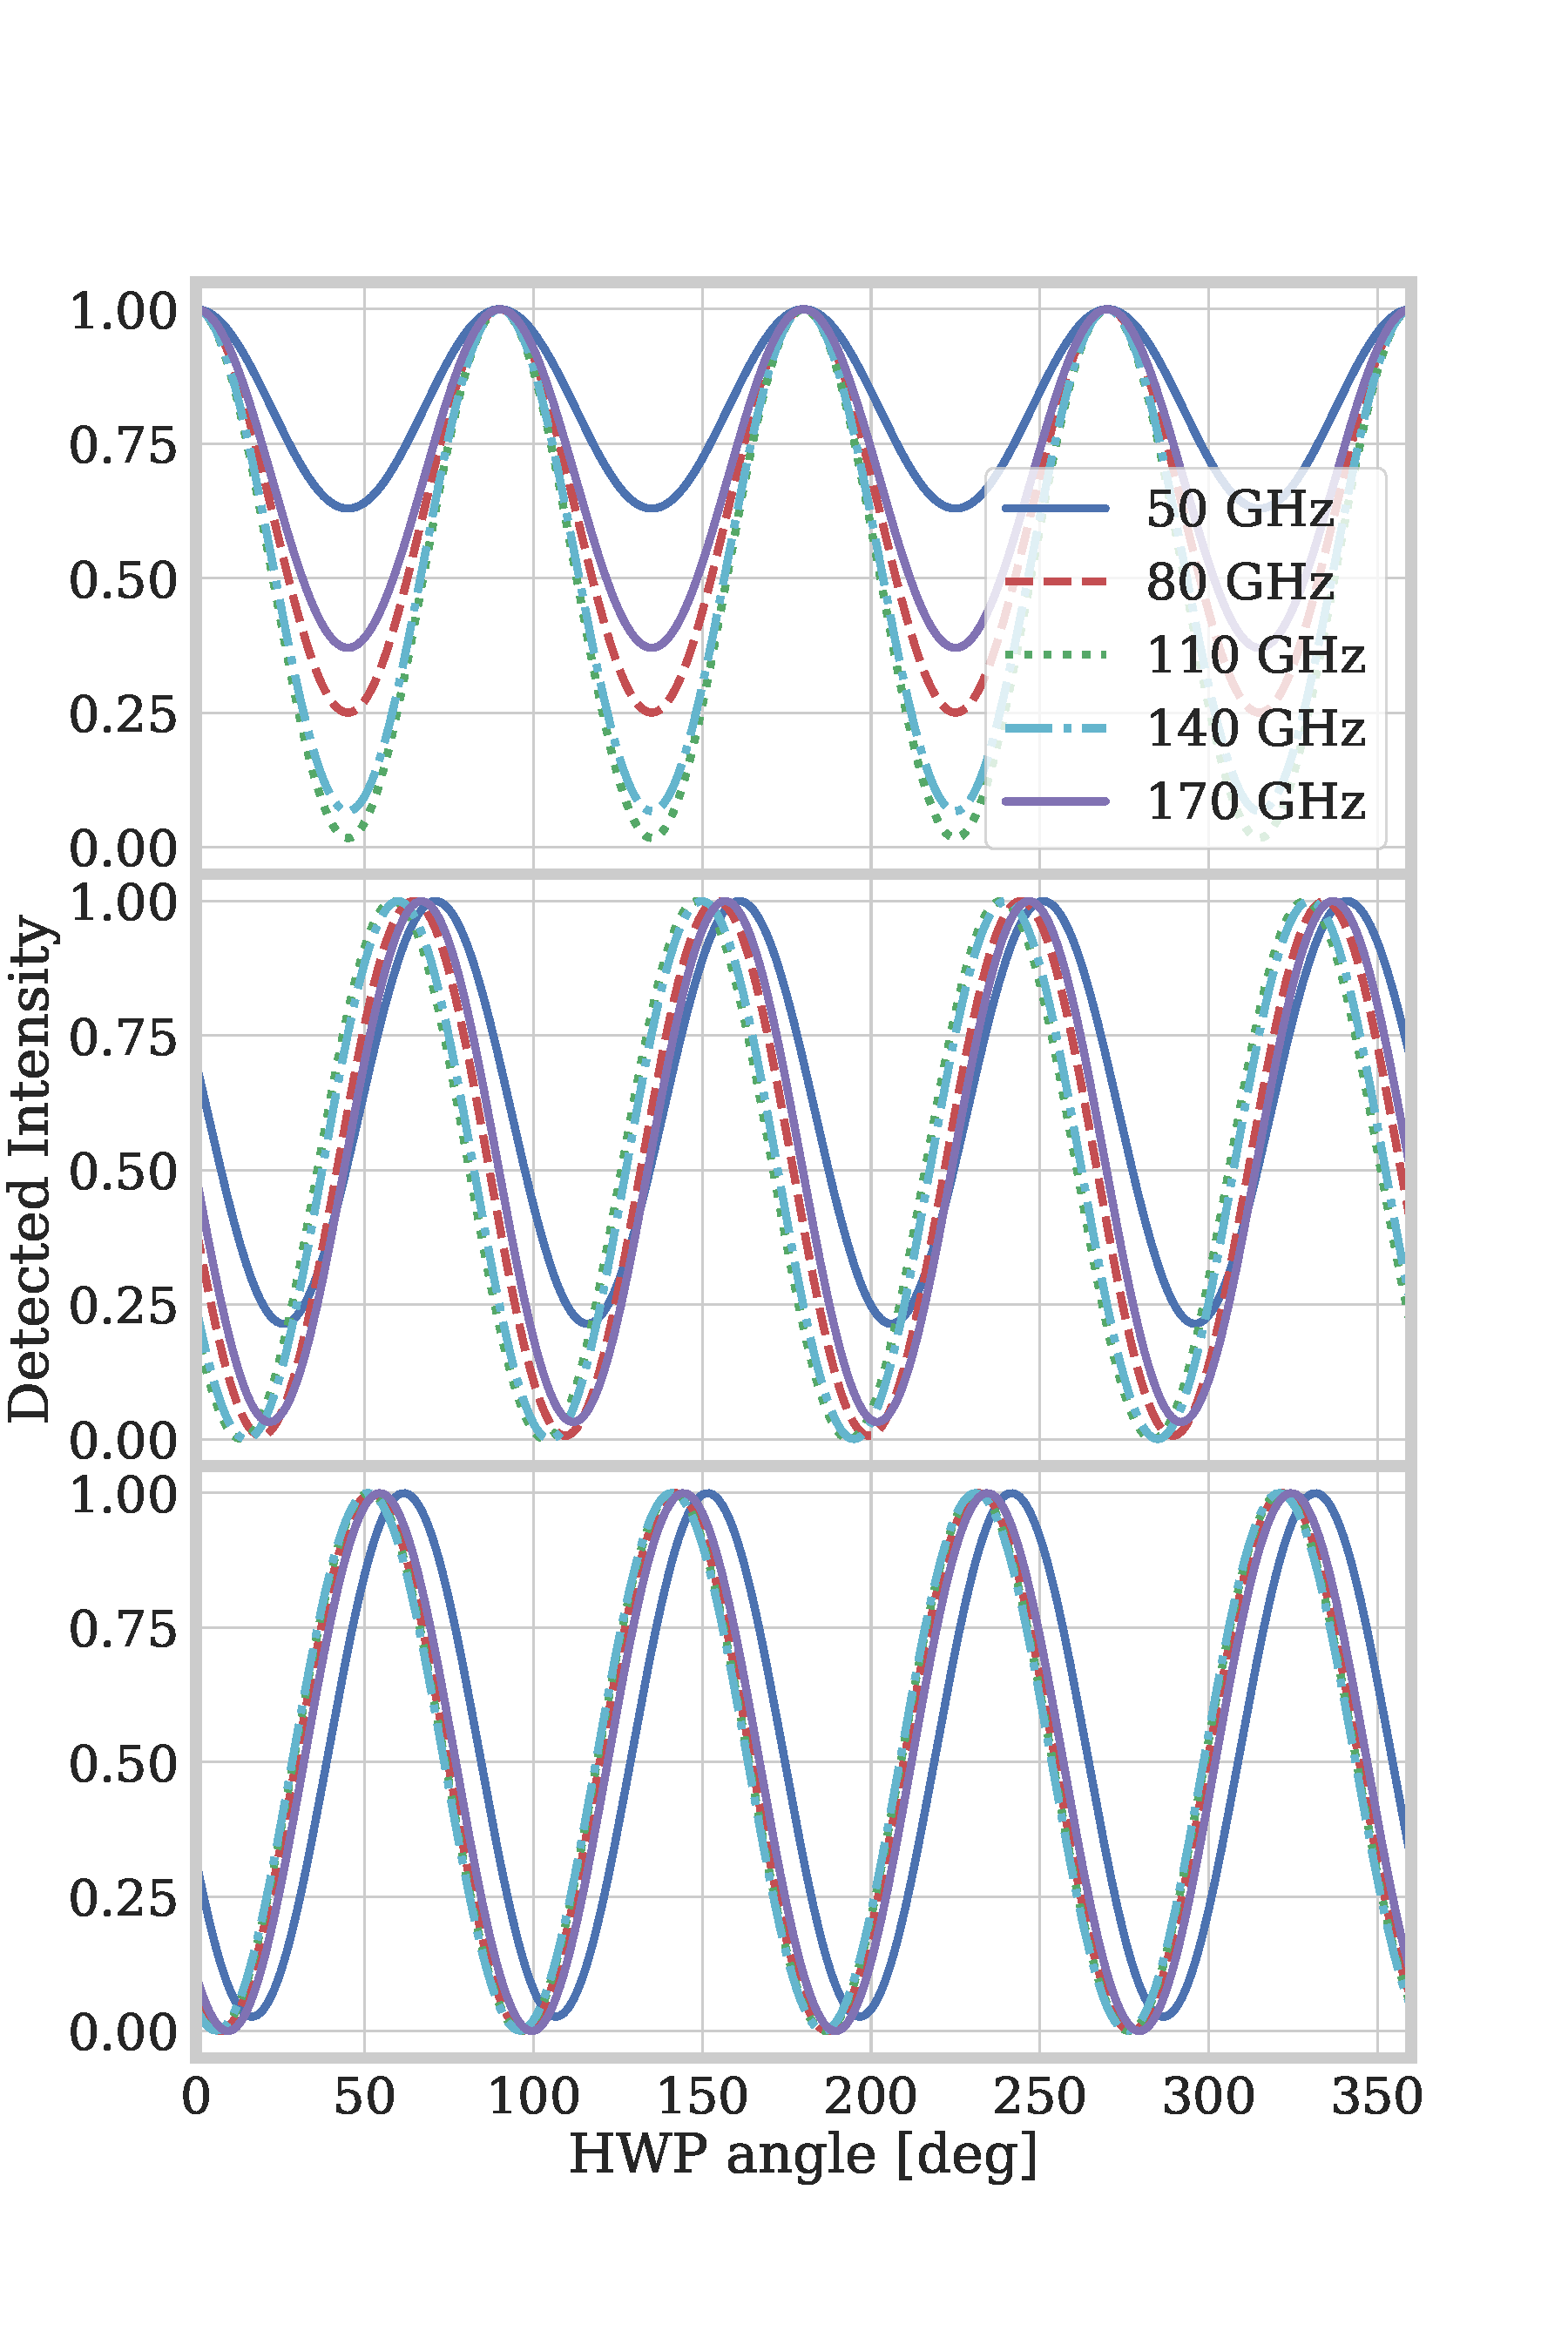
\includegraphics[width=0.6\linewidth, trim=0cm 3cm 2cm 5cm, clip]{PolarizationModulation/Figures/ahwp_detector_modulation.pdf}
    \caption{Caption}
    \label{fig:ahwp_detector_output}
\end{figure}

Consider linearly polarized light $\vec{S}_{\mathrm{in}}$ generated by a narrow-band source that can sweep in frequency, as suggested by Figure~blah, illuminating a HWP with $m$ plates which in turn rotates the output light $\vec{S}_{\mathrm{out}}$ detected by a polarimeter $\vec{d}$. The detector can be modeled using the Mueller matrix
\begin{equation}
    G
    =
    \frac{1}{2}
    \begin{pmatrix}
    1 & 1 & 0 & 0 \\
    1 & 1 & 0 & 0 \\
    0 & 0 & 0 & 0 \\
    0 & 0 & 0 & 0 \\
    \end{pmatrix}
    \label{eq:detector_mueller_matrix}
\end{equation}
such that the detected signal is
\begin{equation}
    \vec{S}_{\mathrm{det}} = G \vec{S}_{\mathrm{out}} \, .
    \label{eq:detected_modulated_power}
\end{equation}
The effect of the polarimeter matrix $G$ is to admit intensity $I_{\mathrm{out}}$ and polarization $Q_{\mathrm{out}}$, but from the detector's perspective, it is simply seeing a modulating power as the HWP rotates. In the case of fully polarized output light $I_{\mathrm{out}} = \sqrt{Q_{\mathrm{out}}^{2} + U_{\mathrm{out}}^{2}}$, the detected power will swing between $[0, I_{\mathrm{out}}]$, but in the case of partially polarized light, the detected power will swing between $[(1 - P_{\mathrm{out}}) I_{\mathrm{out}}, I_{\mathrm{out}}]$, where again $P_{\mathrm{out}}$ is the output polarization fraction. Therefore, we can write the HWP modulation efficiency in terms of the detected intensity as
\begin{equation}
    \varepsilon_{\mathrm{mod}} = \frac{I_{\mathrm{det, max}} - I_{\mathrm{det, min}}}{I_{\mathrm{det, max}} + I_{\mathrm{det, min}}} \, ,
\end{equation}
where $I_{\mathrm{out, max}}$ and $I_{\mathrm{out, min}}$ are the maximum and minimum detected power, respectively.

In the following subsections, we briefly overview the calculation of modulation efficiency and phase for the AHWP at normal incidence and within the context of SA and SO's 90 and 150~GHz bands. However, the topic of AHWP performance is richly studied, and we encourage the interested reader to review published literature to learn about other effects, such as the impacts of increasing detection bandwidth, intensity to polarization leakage, effects at non-normal incidence, stack orientation optimization, among many other topics.

%%%%%%%%%%%%%%%%%%%%%%%%%%%%%%%%
%%%%%%%%%%%%%%%%%%%%%%%%%%%%%%%%

\subsection{Modulation efficiency}
\label{sec:modulation_efficiency}

\iffalse
\begin{figure}
    \centering
    \subfloat[\label{fig:ahwp_detector_output:a}]{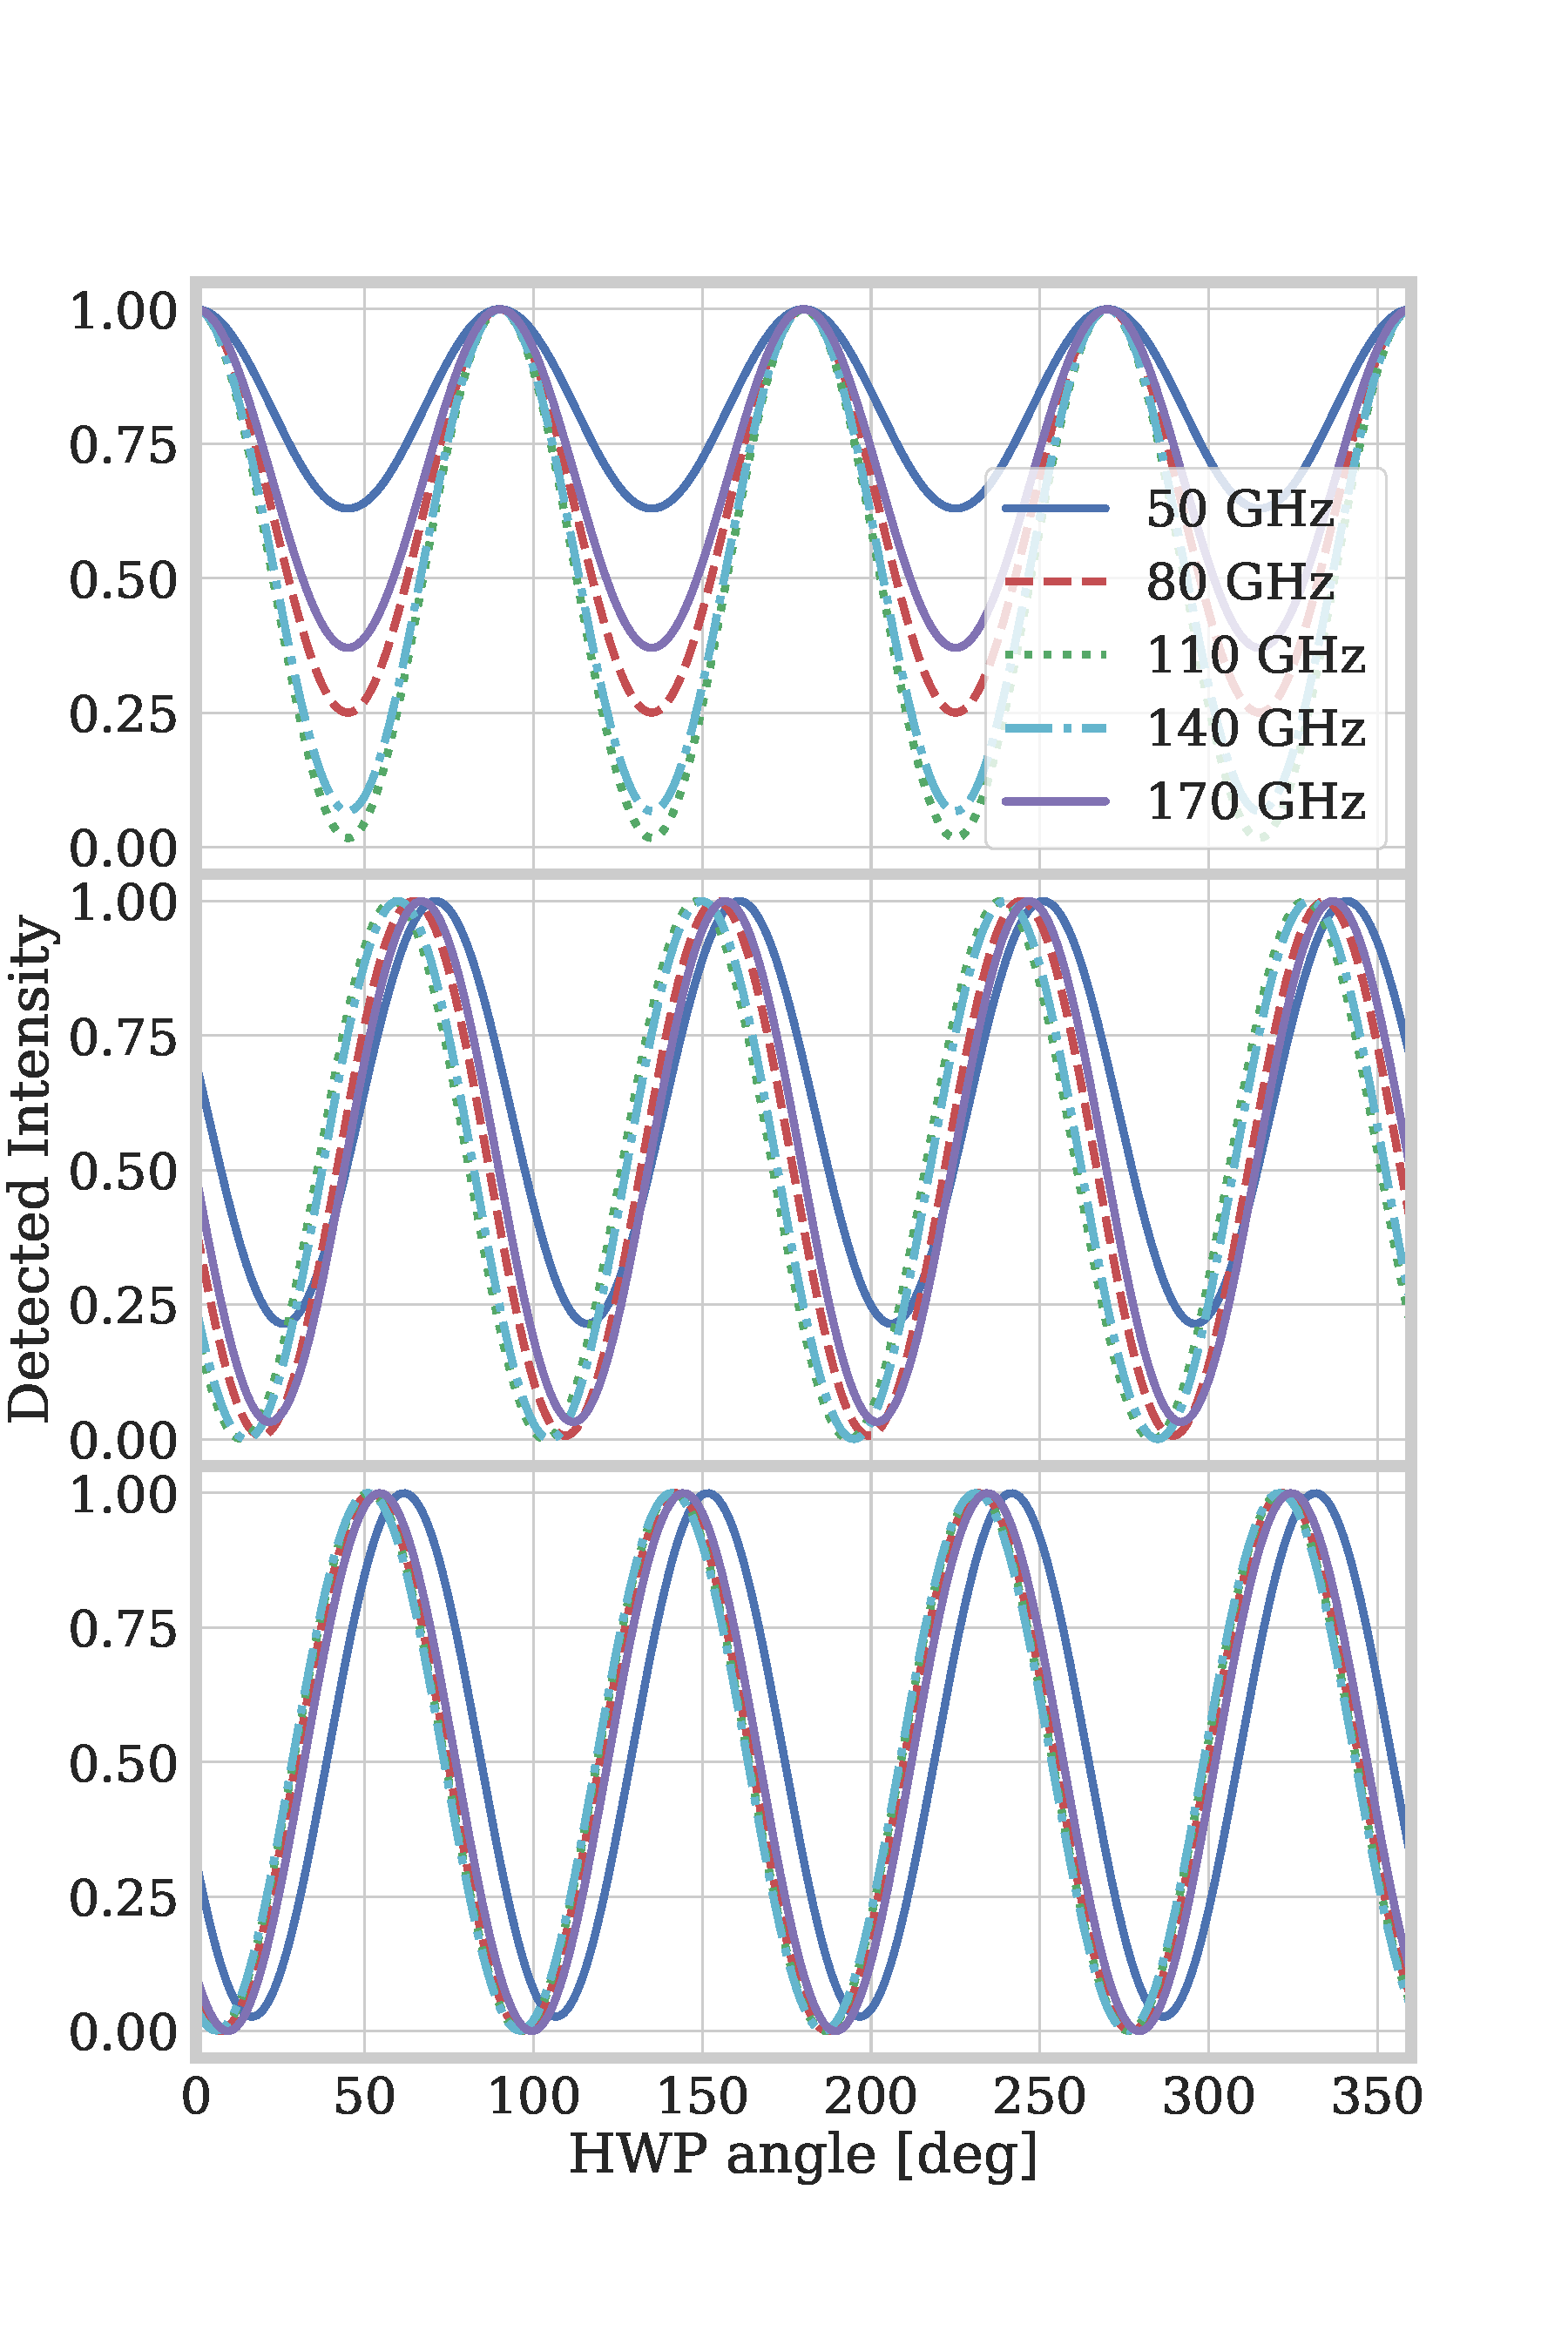
\includegraphics[width=0.48\linewidth, trim=0cm 3cm 2cm 3cm, clip]{PolarizationModulation/Figures/ahwp_detector_modulation.pdf}}
    \subfloat[\label{fig:ahwp_detector_output:b}]{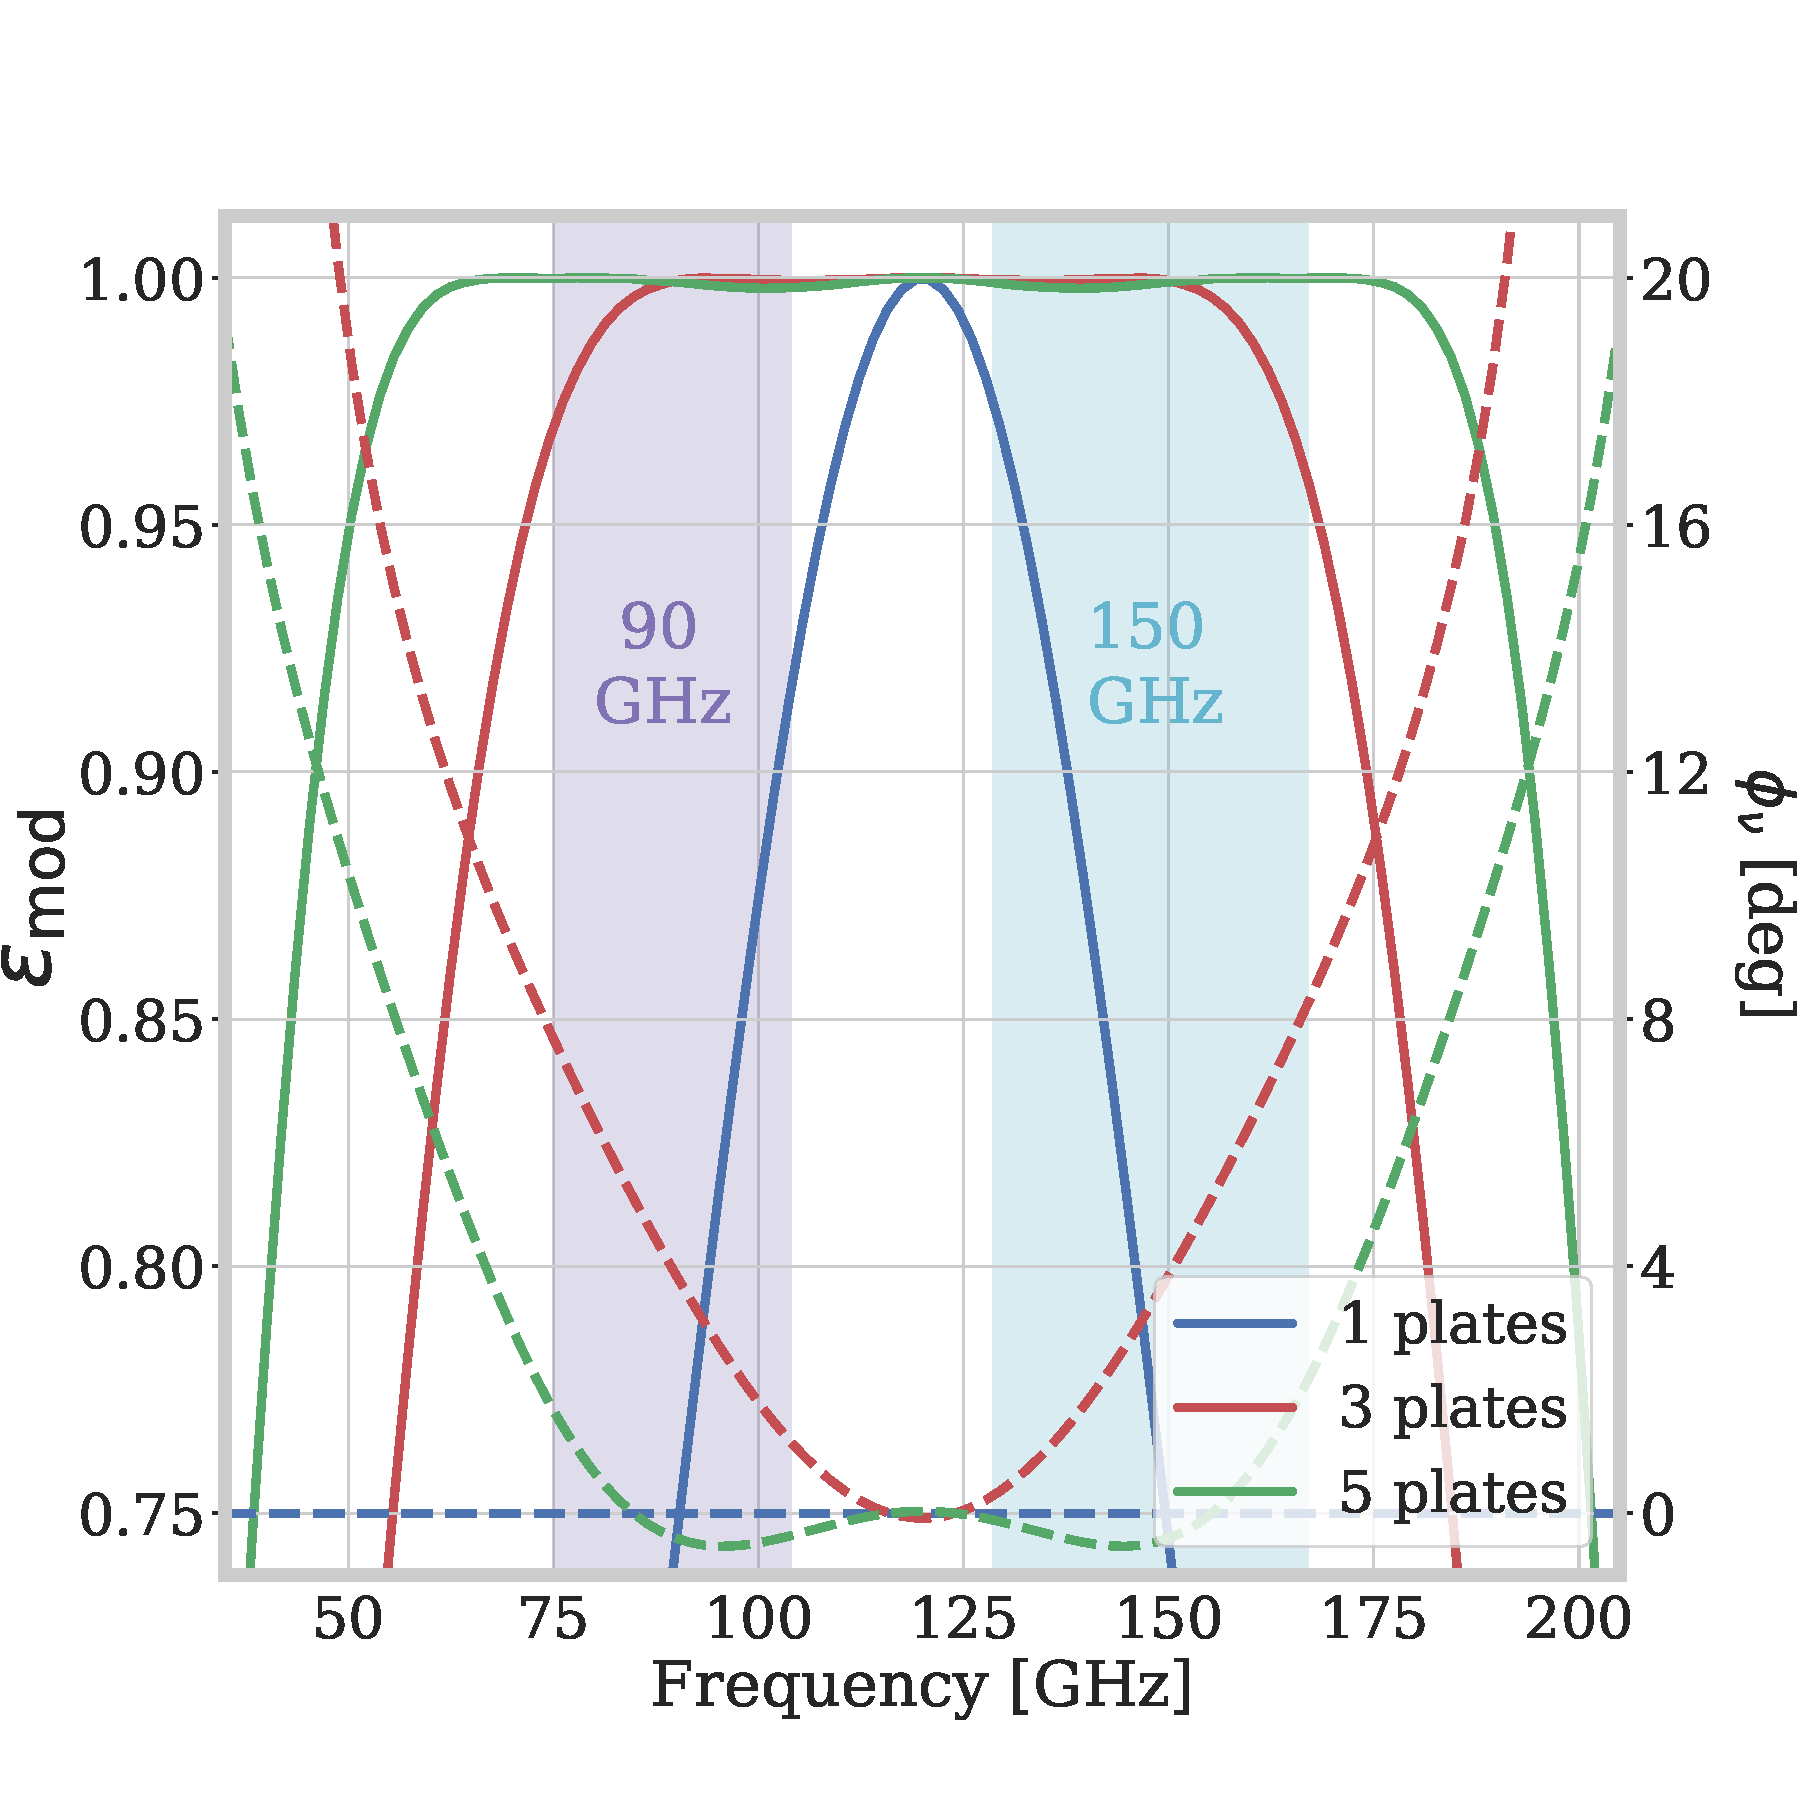
\includegraphics[width=0.48\linewidth, trim=0cm -5.5cm 0cm 2cm, clip]{PolarizationModulation/Figures/one_three_five_plates_modulation_efficiency_phase.pdf}}
    \caption{Caption}
    \label{fig:ahwp_detector_output}
\end{figure}
\fi

\begin{figure}[!t]
    \centering
    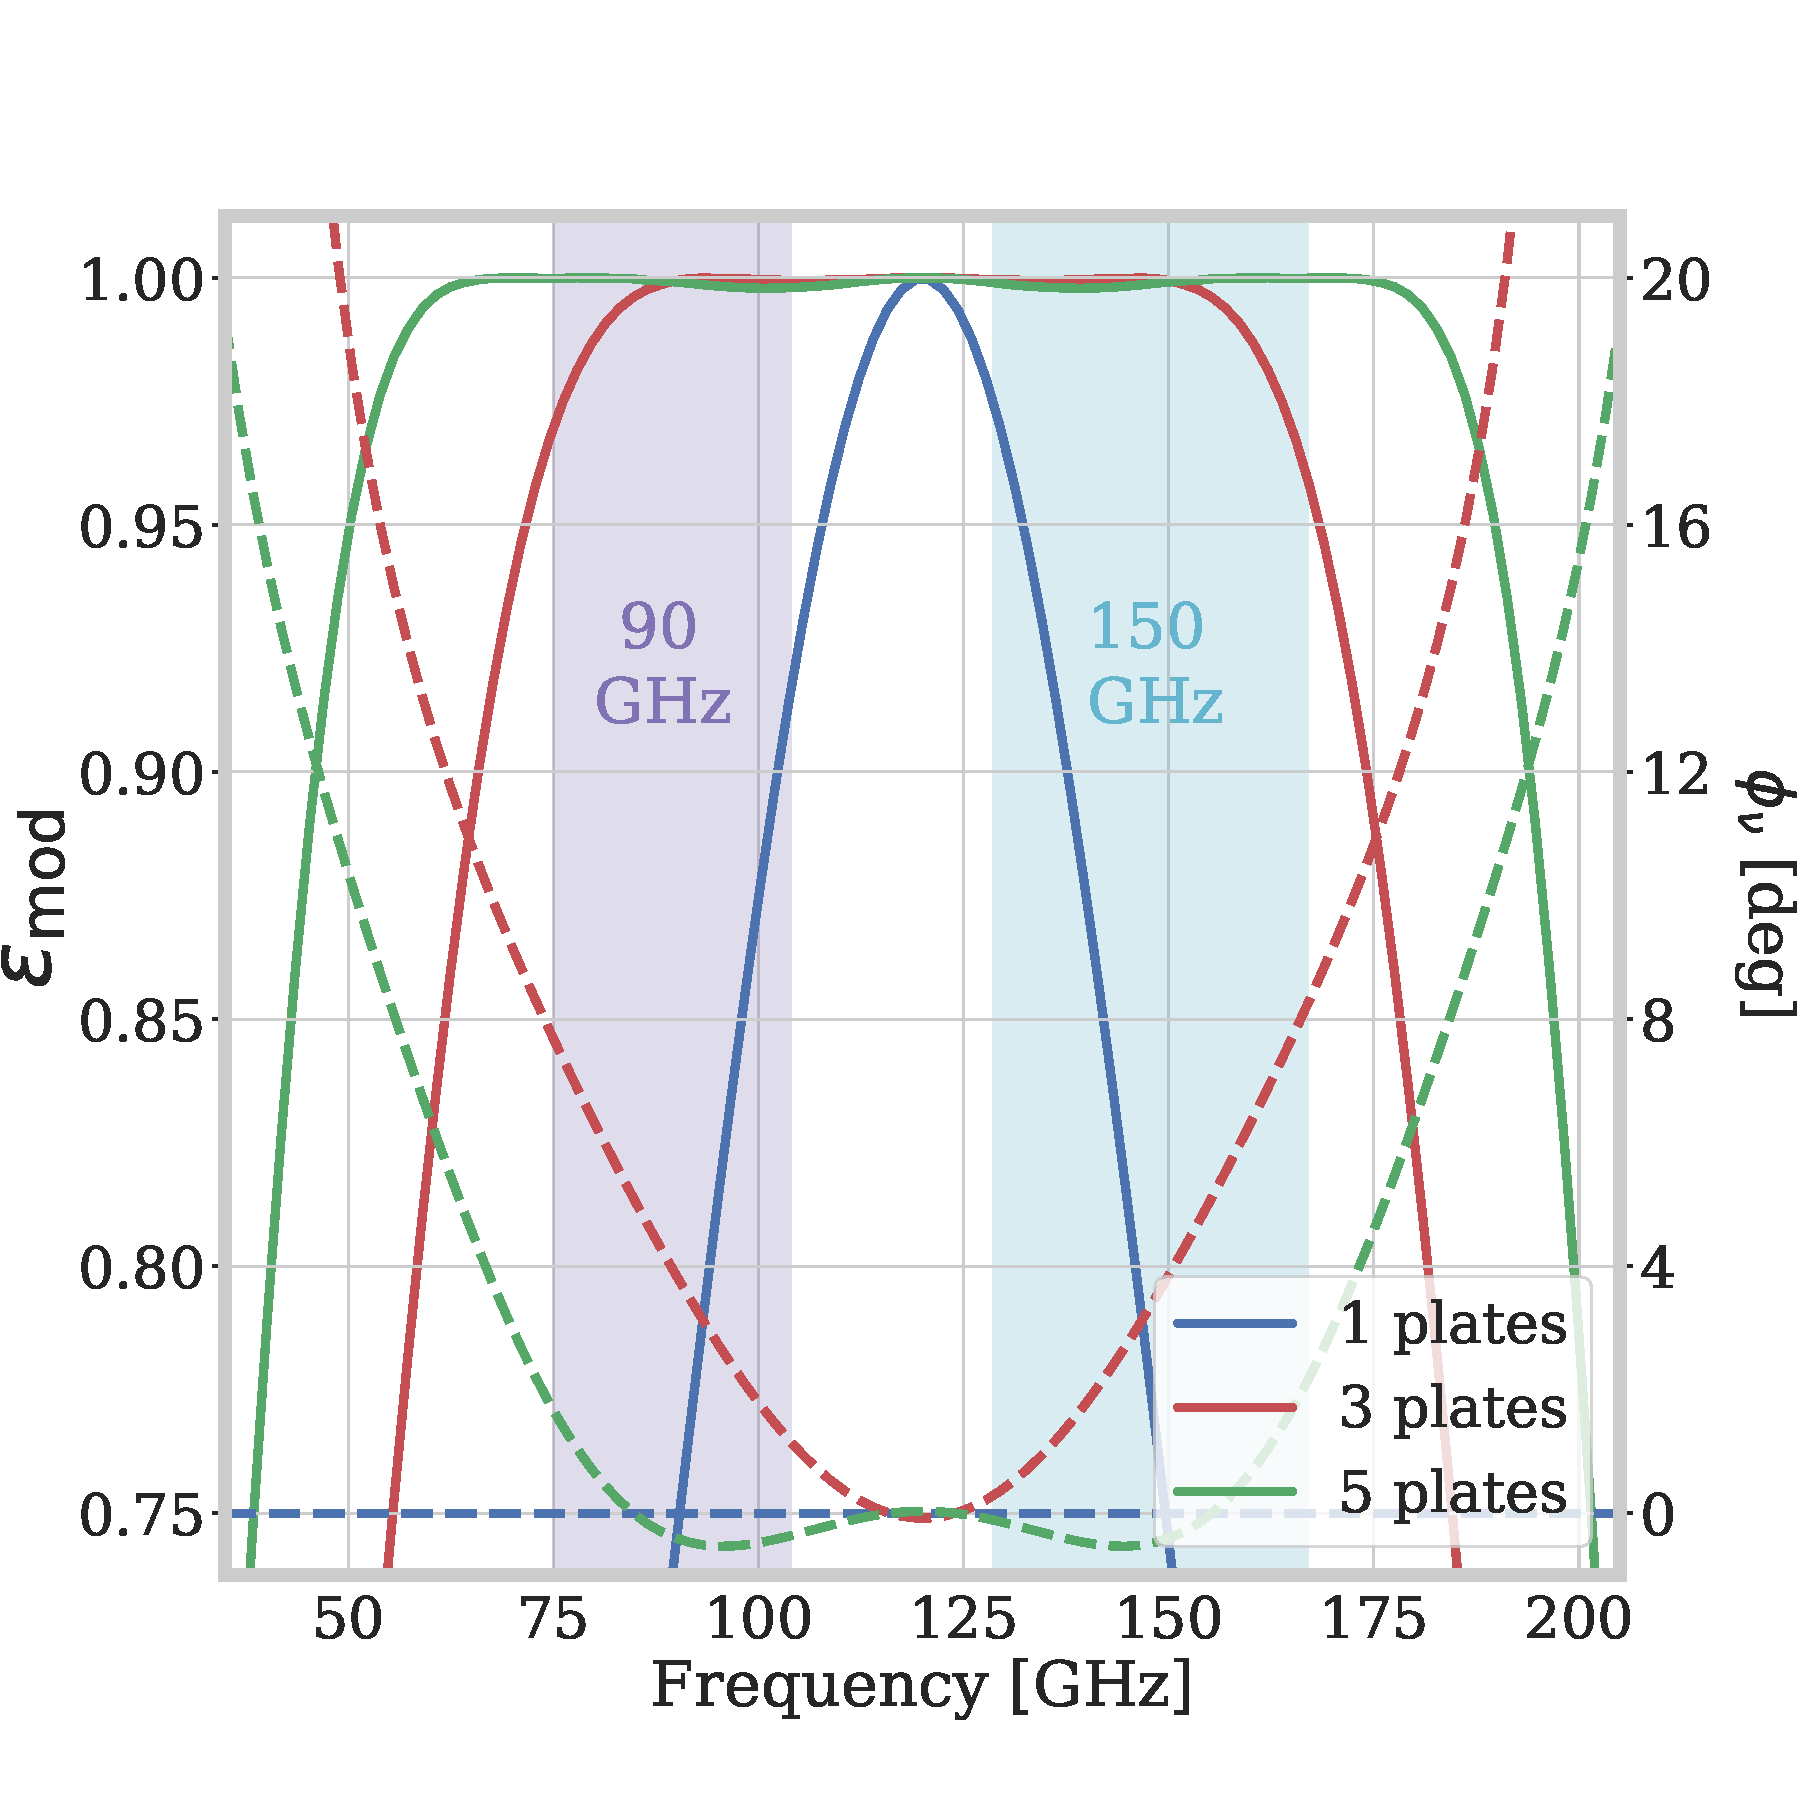
\includegraphics[width=0.7\linewidth, trim=0cm 1cm 0cm 3cm, clip]{PolarizationModulation/Figures/one_three_five_plates_modulation_efficiency_phase.pdf}
    \caption{Caption}
    \label{fig:my_label}
\end{figure}

Figure~blah shows $I_{\mathrm{out}}$ and the resulting $\varepsilon_{mod}$ as a function of frequency for one-, three-, and five-stack HWP along side the band-integrated detected intensity
\begin{equation}
    \left< I_{\mathrm{det}} \right> = \int_{0}^{\infty} I_{\mathrm{det}}(\nu) B(\nu) \dd \nu \, ,
\end{equation}
where here, $B(\nu)$ is the detector band. The resulting modulation efficiencies for the one-, three-, and five-stack scenarios are shown as part of Table~blah. There are several features that are worth pointing out from this study. First, a single-stack HWP has insufficient bandwidth for the PB2 bands (and by extension, the SO MF bands), giving rise to a $\approx$~25\% polarization efficiency loss in both the 90 and 150~GHz bands. This problem is exacerbated by thickness and index tolerances, which will inevitably move the $\varepsilon_{\mathrm{mod}}$ band higher/lower in frequency and therefore favor the 150/90~GHz band over the other. Second, the modulation efficiency gain of a five-stack HWP vs. a three-stack is small, and because a five-stack configuration is thicker and therefore more absorptive/emissive (see Equation~\ref{eq:dielectric_emissivity}), the three-stack is favored for SA and SO's dichroic receivers. Third, there is an apparent phase shift between the 90 and 150~GHz $\left< I_{\mathrm{det}} \right>$ vs. $\rho$ AHWP curves that isn't present for the single-stack configuration. This shift is an important feature of the AHWP which we discuss in the following subsection.

%%%%%%%%%%%%%%%%%%%%%%%%%%%%%%%%
%%%%%%%%%%%%%%%%%%%%%%%%%%%%%%%%

\subsection{Frequency-dependent phase}
\label{sec:frequency_dependent_phase}

The $\left< I_{\mathrm{det}} \right>$ vs. $\rho$ curves in Figure~blah can be modeled via the relation
\begin{equation}
    \left< I_{\mathrm{det}} \right> = \frac{I_{\mathrm{in}}}{2} \left[1  + \varepsilon_{\mathrm{mod}} P_{\mathrm{in}}  \cos \left( 4 \rho - 2 \alpha_{\mathrm{in}} - 4 \phi_{\nu} \right) \right] \, .
    \label{eq:analytic_function_fit_modulated_intensity}
\end{equation}
where here $\left< I_{\mathrm{in}} \right>$ is the input intensity integrated over the detector band $B(\nu)$. We can invert this relationship to write an analytic function for the frequency-dependent phase
\begin{equation}
    \phi_{\nu} = -\frac{1}{4} \arccos \left[ \frac{2 \left< I_{\mathrm{det}} \right> / \left< I_{\mathrm{in}} \right> - 1}{\varepsilon_{\mathrm{mod}} P_{\mathrm{in}}} \right] + \rho - \frac{1}{2} \alpha_{\mathrm{in}} \, .
    \label{eq:modulation_phase_function}
\end{equation}
Phase vs. frequency for the one-, three-, and five-stack HWPs are plotted in Figure~blah, and the band-integrated phases are shown as part of Table~blah.

The effect of the frequency-dependent phase is to rotate the detected polarization angle as a function of frequency. This polarization rotation is called \important{cross polarization} and is of critical importance to an accurate measurement of E-modes and B-modes. The topic of frequency-dependent polarization angle effects in CMB telescopes is an intensively studied topic, and an accurate understanding about how such effects can leak E-modes into B-modes---a phenomenon referred to as \important{EB leakage}---requires a full blown instrument simulation. However, we can gain some intuition from a relatively simple analysis that also gives an accurate leakage estimate.

The \textit{true} $Q$ and $U$ sky signals are modified by a global polarization angle rotation of $\Delta \alpha$ as
\begin{eqnarray}
    \left[ Q + i U \right]' & = & e^{-2 i \Delta \alpha} \left[ Q + i U \right] \nonumber \\
    \left[ Q - i U \right]' & = & e^{-2 i \Delta \alpha} \left[ Q - i U \right] \, .
\end{eqnarray}
As discussed in Section~\ref{sec:anisotropies}, we can decompose these these linear combinations of $Q$ and $U$ into spherical harmonics as
\begin{eqnarray}
    a_{2, \ell m} & = & \int \dd \Omega\,  Y^{*}_{\ell m}\left( \hat{n} \right) \left[ Q + i U \right]\left( \hat{n} \right) \nonumber \\
    a_{-2, \ell m} & = & \int \dd \Omega \, Y^{*}_{\ell m}\left( \hat{n} \right) \left[ Q - i U \right]\left( \hat{n} \right)
    \label{eq:alm_QU}
\end{eqnarray}
and the B-mode Fourier amplitude is written as
\begin{equation}
    a_{B, \ell m} = i \left[ a_{2, \ell m} - a_{-2, \ell m} \right] \, ,
    \label{eq:alm_B}
\end{equation}
such that the B-mode power spectrum amplitude is
\begin{equation}
    C_{\ell}^{BB} = \left< a_{B, \ell m} \, a_{B, \ell m}^{*} \right> \, ,
\end{equation}
where the angle brackets denote the statistical average. Using these these relationships, we can quantify the shift in the power spectrum as
\begin{equation}
    \mathrm{Bias}\left[ C_{\ell}^{BB} \right] \equiv \frac{C_{\ell}^{BB} - C_{\ell}^{BB \prime}}{C_{\ell}^{BB}} = \frac{\left( a_{2, \ell m}^{\prime} - a_{-2, \ell m}^{\prime} \right)^{2} - \left( a_{2, \ell m} - a_{-2, \ell m} \right)^{2}}{\left( a_{2, \ell m} - a_{-2, \ell m} \right)^{2}} \, .
    \label{eq:C_ell_BB_bias_modulation_phase}
\end{equation}
In general, a proper estimation of the BB bias due to polarization angle rotation $\mathrm{Bias}\left[ C_{\ell}^{BB} \right]$ requires an end-to-end simulation pipeline that accounts for how the detector data is filtered, how the maps are constructed, and how the power spectrum is calculated, especially because there are many other steps in the analysis process that can introduce their own EB leakage. However, we can make a very simple estimate by plugging $a_{2, \ell m} = [ Q + i U ]$, $a_{-2, \ell m} = [ Q - i U ]$, $a_{2, \ell m}' = [ Q + i U ] \exp[2 i \Delta \alpha]$, and $a_{-2, \ell m} = [ Q - i U ] \exp[2 i \Delta \alpha]$ into Equation~\ref{eq:C_ell_BB_bias_modulation_phase}, which allows to extract the simple relation
\begin{equation}
    \mathrm{Bias}\left[ C_{\ell}^{BB} \right] \sim \sin^{2} \left( 2 \Delta \alpha \right) \, .
    \label{eq:C_ell_BB_bias_simplified}
\end{equation}
As shown in Figure~\ref{fig:bb_spectrum}, given that B-mode power is $\gtrsim$~100x smaller than that of E-modes, any miscalibration of the HWP-dependent phase $\Delta \alpha$ needs to be $\lesssim$~1~deg to avoid biasing the BB spectrum in to a meaningful level.

\begin{figure}[!t]
    \centering
    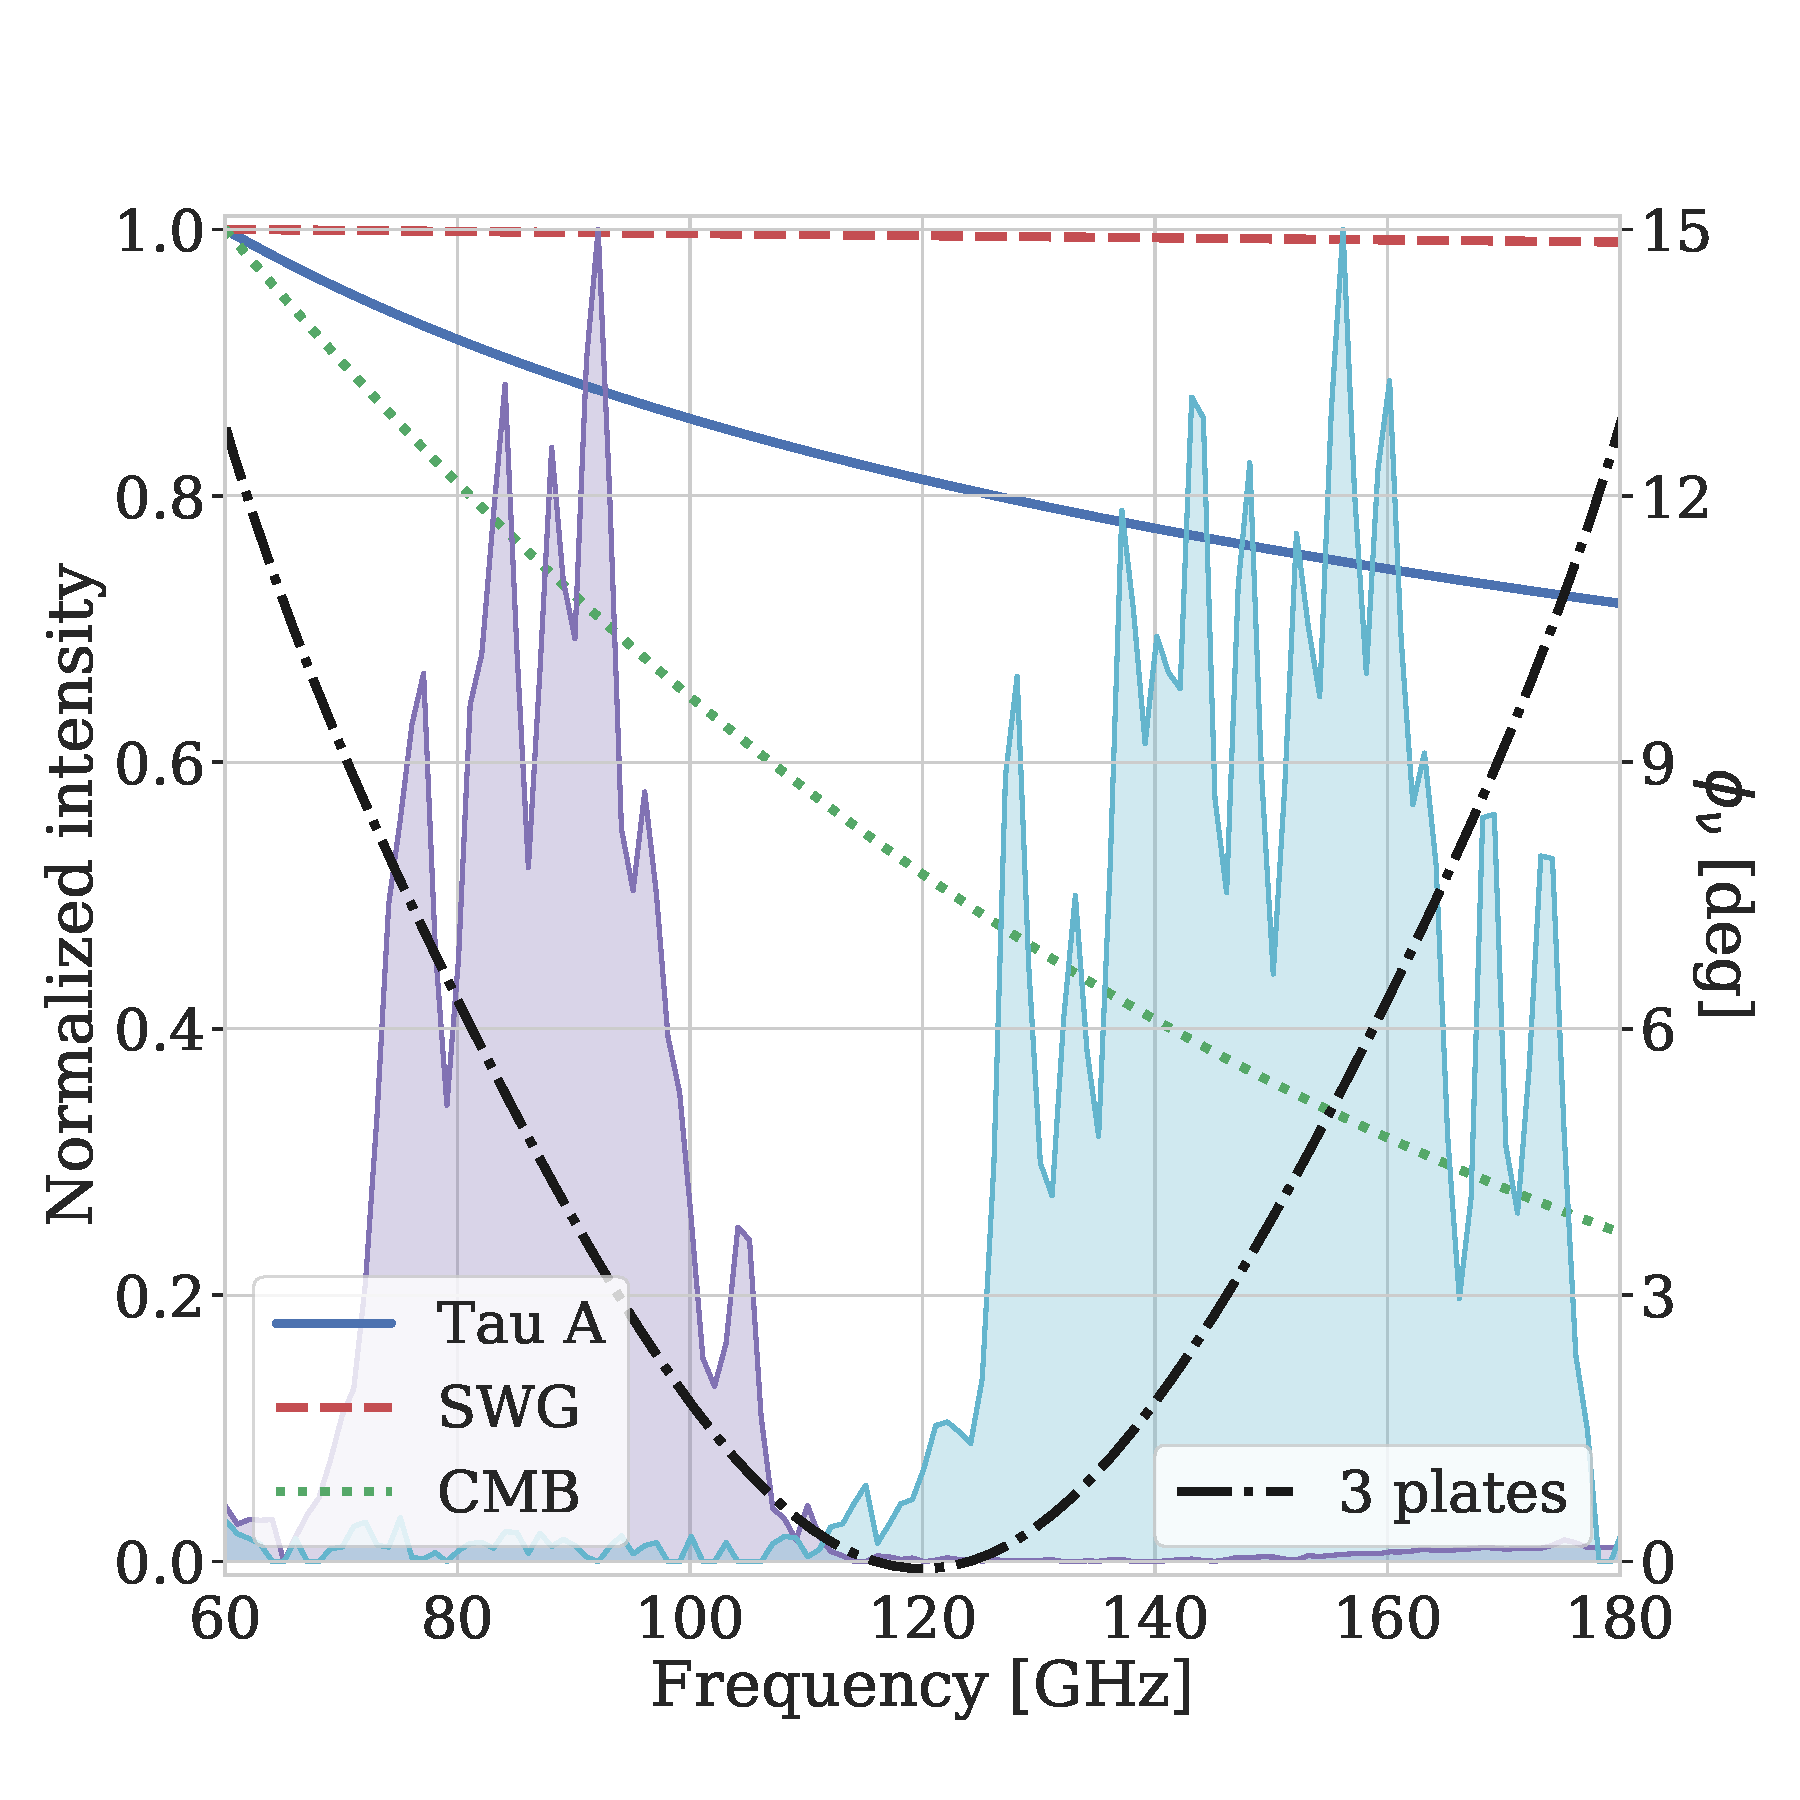
\includegraphics[width=0.6\linewidth, trim=0cm 1cm 0cm 2cm, clip]{PolarizationModulation/Figures/angle_calibration_spectra.pdf}
    \caption{Caption}
    \label{fig:angle_calibration_spectra}
\end{figure}

Using the simple, approximation BB bias estimate given by Equation~\ref{eq:C_ell_BB_bias_simplified}, we can quickly quantify the effectiveness of various angle calibration techniques in mitigating EB leakage. The essential issue is that when using an AHWP, if you measure the polarization angle using a source with a different spectrum than that of the scientific sources---the CMB, galactic dust, and synchrotron emission---you will bias the polarization angle of said sources. In this sense, the problem of raised by the frequency-dependent phase $\phi_{\nu}$ in Equation~\ref{eq:modulation_phase_function} is one of understanding the spectral behaviors of the calibration source's spectrum.

Consider three methods for polarization calibration
\begin{enumerate}
    \item Self-calibration. This technique assumes a priori that there is no cosmic birefringence that could correlate CMB E-mode and B-mode polarization and therefore nulls $C_{\ell}^{EB}$ to calibrate the polarization angle.
    \item Calibration using a celestial source. Tau-A is a polarized supernova remnant that is bright at mm wavelengths and small enough to be a point source for the angular resolutions of most mm-wave telescopes. 
    \item Calibration using a terrestrial source. There are many techniques to use a man-made source to measure polarization that vary substantially with telescope aperture size, but we will highlight one method that was conceptually demonstrated on POLARBEAR, which is to reflect emission from the ground (which is $\sim$~300~K) from a sparse wire grid (SWG) to generate a small polarized signal.
\end{enumerate}
The diffraction-limited, single-moded, detected power spectra from Tau-A and the sparse wire grid are
\begin{eqnarray}
    p_{\mathrm{CMB}}(\nu) & = & \varepsilon_{\mathrm{CMB}} \frac{h \nu}{e^{h \nu / ( k_{\mathrm{B}} T_{\mathrm{CMB}} )} - 1} \\
    p_{\mathrm{\tau A}}(\nu) & = & A_{\mathrm{\tau A}} + B_{\mathrm{\tau A}} \nu^{\beta_{\mathrm{\tau A}}} \\
    p_{\mathrm{SWG}}(\nu) & = & \varepsilon_{\mathrm{SWG}} \frac{h \nu}{e^{h \nu / ( k_{\mathrm{B}} T_{\mathrm{gnd}} )} - 1} \, .
   \label{eq:tau_a_spectrum}
\end{eqnarray}
The first equation is that of the CMB with a polarization fraction $\varepsilon_{\mathrm{CMB}}$ that is assumed to be frequency independent.
In the second equation, $A_{\mathrm{\tau A}}$ and $B_{\mathrm{\tau A}}$ are Tau-A coefficients that give units of W / Hz, and $\beta_{\mathrm{\tau A}}$ is the spectral index, which according to blah is $\beta_{\mathrm{\tau A}} \approx -0.3$. The final equation is simply that of a blackbody with temperature of the Earth $T_{\mathrm{ground}}$, modified by the sparse wire grid's polarizing efficiency $\varepsilon_{\mathrm{SWG}}$. 

To inspect the possible miscalibration of the CMB polarization angle when calibrating that of the telescope using Tau-A and the SWG, we integrate the frequency-dependent phase over the detector band, weighted by the calibration spectrum, to find the a band-averaged instrument angle
\begin{equation}
    \alpha_{\mathrm{inst}} = \frac{\int_{0}^{\infty} \phi(\nu) B(\nu) p(\nu) \dd \nu}{\int_{0}^{\infty} B(\nu) p(\nu) \dd \nu} \, ,
    \label{eq:band_averaged_polarization_angle}
\end{equation}
where $B(\nu)$ is the detector band, $p(\nu)$ is the spectrum of the calibration source, and the frequency-dependent phase for the AHWP is given by Equation~\ref{eq:modulation_phase_function}. The results of the band-averaged angles for the 90 and 150~GHz bands (the primary CMB channels) are given in Table~\ref{tab:ahwp_angle_calibration_error}.

\begin{table}[!t]
    \centering
    \begin{tabular}{c|c|c}
        \hline
        Channel &  Tau-A $\Delta \alpha$ & SWG $\Delta \alpha$ [deg] \\
        \hline
        \hline
        90~GHz & 0.4 & -0.2 \\
        \hline
        150~GHz & 0.0 & 0.6 \\
        \hline
    \end{tabular}
    \caption{Angle calibration errors in the measurement of CMB polarization induced by using a three-stack HWP and either Tau-A or a sparse-wire-grid calibrator to measure the instrument's polarization angle.}
    \label{tab:ahwp_angle_calibration_error}
\end{table}

There are a few points that ought to be emphasized about this brief overview of the AHWP's frequency-dependent phase. First, this analysis is crude, and more rigorous and studies have been done for EBEX, which employed a five-stack AHWP for balloon-borne CMB observation, and for SO. However, the general conclusions are the same as we have shown here, which that even with no mitigation techniques, the BB bias introduced by the AHWP's frequency-dependent rotation is small. In fact, the typical uncertainty in the angle calibration of existing CMB experiments, such as POLARBEAR and ACT, is a the $\sim$~1~deg level, and therefore the addition of an AHWP to demonstrated optical systems is not expected to be a forbidding issue for SA and SO. Second, the problem presented here for CMB calibration is also true for foreground subtraction. Because dust and synchrotron emission have different spectra than the CMB, frequency-dependent angle effects need to be taken into account during component separation. We have not used Equation~\ref{eq:band_averaged_polarization_angle} to calculate dust angles, as the physics and analysis techniques surrounding foregrounds is beyond the scope of this discussion, but it is worth noting that having separate frequency channels to monitor foregrounds, in which the angle can be calibrated individually, is of crucial importance to correctly measuring contaminating polarization angles, adding another motivation for deploying many frequencies in a given observatory.

It is also worth noting that while these frequency-dependent effects have been deemed subdominant for SA and SO, they could become important for future missions with tighter systematic error budgets. Therefore, there is ongoing research into how AHWPs can be constructed to have a frequency-\textit{independent} angle, and the LiteBIRD team in particular has made substantial progress in this area. Finally, we have not included a comparison of $\Delta \alpha$ for the sinuous, which also has a wobble, because SA and SO use a technique called \important{wobble cancellation} to mitigate the frequency-dependent angle of the antennas. Because the sinuous antenna's meandering design has a handedness, half of the detectors on the array are mirrored, and therefore have a polarization wobble which is the inverse of its non-mirrored partners. Therefore, when maps from various detectors are coadded, the polarization, in principle, cancels, mitigating its effect. Early characterization of PB-2a has shown this technique to be working as expected, and therefore even though the sinuous and AHWP phase drifts are similar, the AHWP was generally (but not always) a greater focus during SA angle calibration studies.

%%%%%%%%%%%%%%%%%%%%%%%%%%%%%%%%
%%%%%%%%%%%%%%%%%%%%%%%%%%%%%%%%
%%%%%%%%%%%%%%%%%%%%%%%%%%%%%%%%

\section{Continuous polarization modulation}
\label{sec:continuous_polarization_modulation}

There are two modes of HWP polarization modulation. One method is to use a \important{stepped HWP}, which involves rotating the HWP in discrete steps between observations. This technique allows sky polarization to be observed with various global rotations, which is a powerful tool to separate cosmic polarization from that generated by the instrument. It also allows orthogonal polarimeters to measure the same sky polarization, providing a cross check of a various beam systematics. While the stepped half-wave plate mitigates beam systematics discussed in Section~blah, it does not mitigate 1/f atmospheric fluctuations, and therefore ground-based experiments often turn to the \important{continuously rotating HWP}.

\begin{figure}[!t]
    \centering
    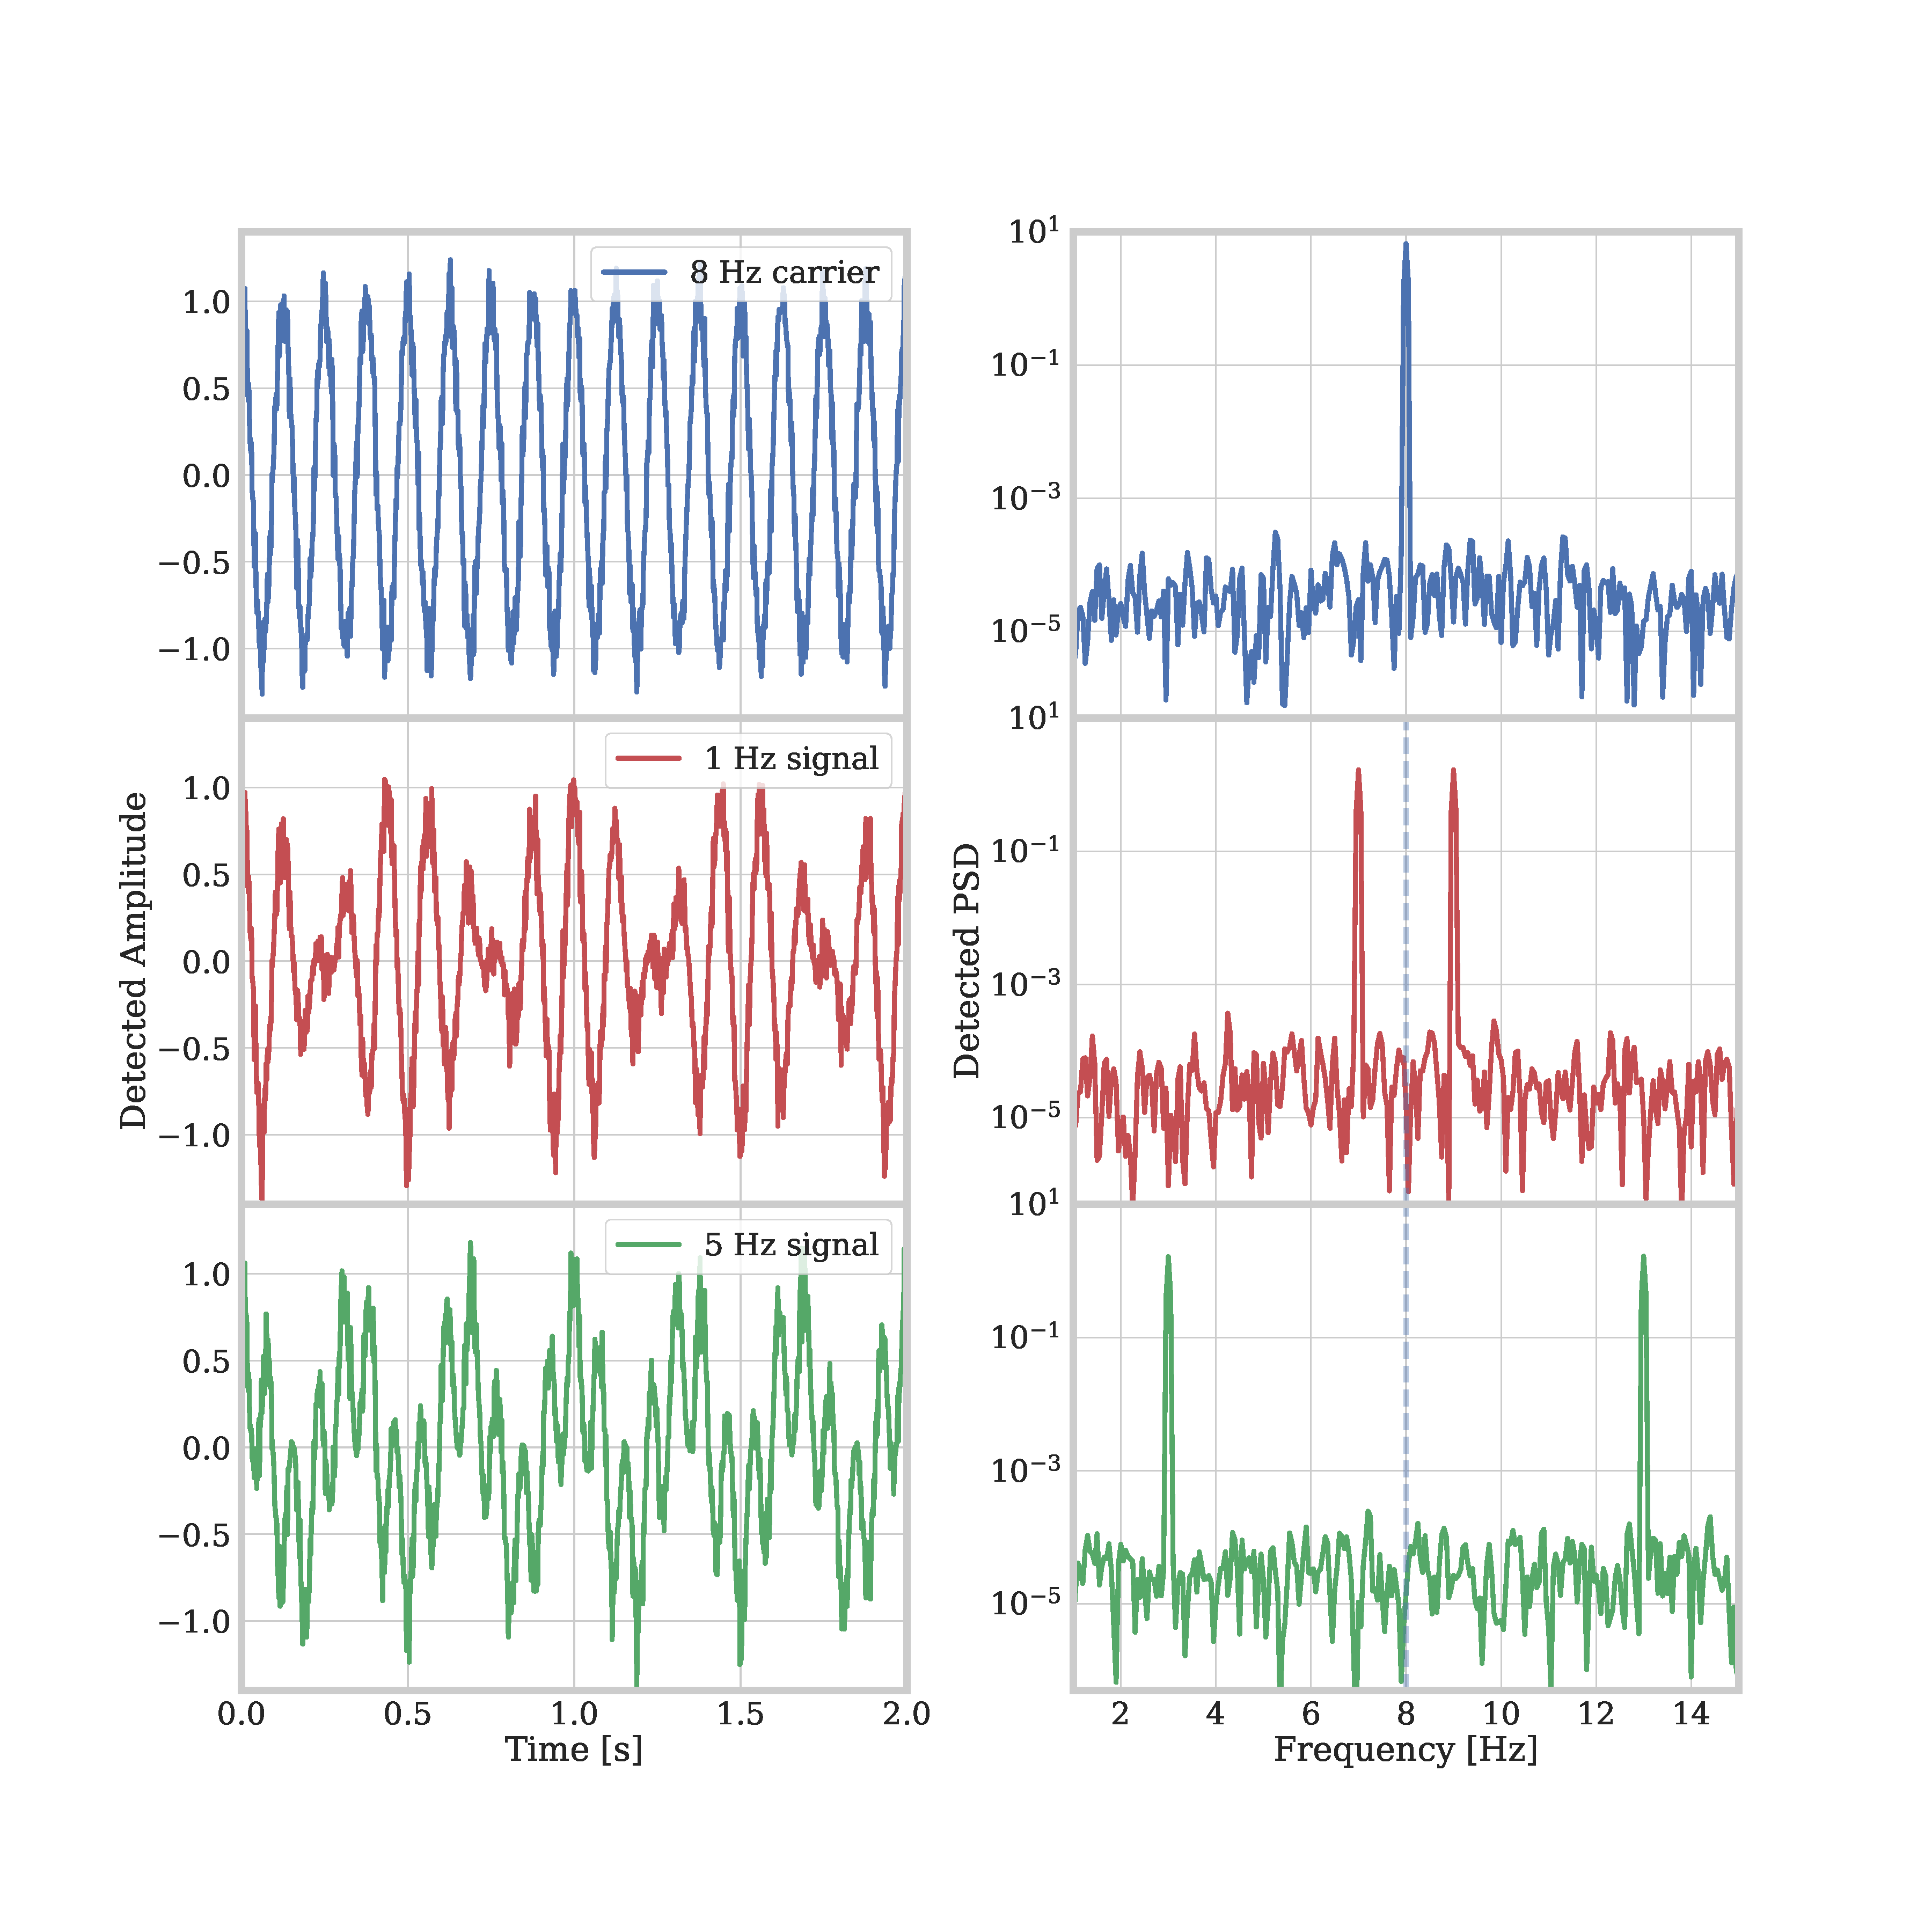
\includegraphics[width=0.7\linewidth, trim=5cm 5cm 5cm 5cm, clip]{PolarizationModulation/Figures/amplitude_modulation_demo.pdf}
    \caption{A toy demonstration of amplitude modulation.}
    \label{fig:amplitude_modulation}
\end{figure}

SA and SO use continuously rotating sapphire AHWPs as polarization modulators, which simultaneously mitigate beam systematics and atmospheric 1/f noise. A continuously rotating HWP modulates an input polarized sky signal $[Q_{\mathrm{in}}(t) \pm i U_{\mathrm{in}}(t)]$ onto the a detector with output $d_{\mathrm{m}}(t)$ as
\begin{equation}
    d_{\mathrm{m}}(t) = I_{\mathrm{in}}(t) + \varepsilon_{\mathrm{mod}} \mathrm{Re} \{ \left[ Q_{\mathrm{in}}(t) \pm i U_{\mathrm{in}}(t) \right] \exp \left[ \mp i 4 \chi(t) \right] \} \, ,
    \label{eq:continuous_hwp_modulation_detected}
\end{equation}
where $\chi$ is the HWP rotation angle and $m(\chi) = \exp \left[ \mp i 4 \chi(t) \right]$ is often called the \important{modulation function}. A continuously rotating HWP aims to spin the birefringent stack with a steady velocity
\begin{equation}
    \chi(t) = 2 \pi f_{\mathrm{HWP}} t \, ,
    \label{eq:hwp_angle_frequency}
\end{equation}
such that the modulation frequency is
\begin{equation}
    f_{\mathrm{m}} = 4 f_{\mathrm{HWP}} \, .
    \label{eq:modulation_frequency}
\end{equation}
Equation~\ref{eq:continuous_hwp_modulation_detected} is in the time domain, but it is typically most powerful to conceptualize the HWP's operation in the Fourier domain. To provide some intuition, consider a sky signal composed of a single Fourier mode
\begin{equation}
    \left[ I_{\mathrm{in}} + Q_{\mathrm{in}} \pm U_{\mathrm{in}} \right](t) = \left[ I_{\mathrm{in}} + Q_{\mathrm{in}} \pm U_{\mathrm{in}} \right] \exp \left( i \omega_{\mathrm{sig}} t \right) \, ,
    \label{eq:sky_polarization_signal_single_mode}
\end{equation}
which when Fourier transformed becomes
\begin{equation}
    d_{\mathrm{m}}(\omega_{\mathrm{sig}}) = I(\omega_{\mathrm{sig}}) + \frac{1}{2} \left[ Q_{\mathrm{in}} + i U_{\mathrm{in}} \right](4 \omega_{\mathrm{HWP}} + \omega_{\mathrm{sig}}) +  \frac{1}{2} \left[ Q_{\mathrm{in}} - i U_{\mathrm{in}} \right](4 \omega_{\mathrm{HWP}} - \omega_{\mathrm{sig}}) \, ,
    \label{eq:modulated_detector_output_fourier_domain}
\end{equation}
where here $\omega_{\mathrm{HWP}} = 2 \pi f_{\mathrm{HWP}}$. There are two salient features of Equation~\ref{eq:modulated_detector_output_fourier_domain}. First, the polarized sky signals $\left[ Q_{\mathrm{in}} \pm i U_{\mathrm{in}} \right]$ are moved from frequency $\omega_{\mathrm{sig}}$ to frequencies $4 \omega_{\mathrm{HWP}} \pm \omega_{\mathrm{sig}}$, while the intensity sky signal is left at $\omega_{\mathrm{sig}}$. This is the signature of \important{amplitude modulation}, in which variations in the polarized sky signal modulate the amplitude of the HWP-generated \important{carrier signal} at $4 \omega_{\mathrm{HWP}}$. Stated in the time domain, this phenomenon arises the modulation operation multiplies $\exp(i \omega_{\mathrm{sig}} t)$ by $\exp(i 4 \omega_{\mathrm{HWP}})$, as $\sin(\omega_{\mathrm{sig}} t) \sin(4 \omega_{\mathrm{HWP}} t) = 1/2 [\cos((4 \omega_{\mathrm{HWP}} - \omega_{\mathrm{sig}}) t) - \cos((4 \omega_{\mathrm{HWP}} + \omega_{\mathrm{sig}}) t) ]$. Second, because the sky signals appear at frequencies $\pm \omega_{\mathrm{sig}}$ around the carrier frequency $4 \omega_{\mathrm{HWP}}$, it is important the HWP \important{side bands} $4 \omega_{\mathrm{HWP}} \pm \omega_{\mathrm{sig}}^{\mathrm{max}}$ are in a white-noise-dominated frequency regime. Stated another way, the HWP rotation frequency $f_{\mathrm{HWP}}$ needs to be large enough such that any science signals are up-converted to frequencies above that of the atmospheric 1/f noise. We discuss this requirement in more detail in Sections~blah and~blah.

%%%%%%%%%%%%%%%%%%%%%%%%%%%%%%%%
%%%%%%%%%%%%%%%%%%%%%%%%%%%%%%%%

\subsection{HWP synchronous signals}
\label{sec:hwp_synchronous_signals}

Equation~\ref{eq:continuous_hwp_modulation_detected}, while instructive, is only a portion of the signal from a real HWP. In addition to the modulated sky signal, the HWP generates \important{HWP synchronous signals} (HWPSS), which can be decomposed as
\begin{equation}
    \mathcal{P}_{\mathrm{HWPSS}} = \sum_{n = 1} \mathrm{Re}\{ \left[ A_{n}(t) e^{-i n \chi(t)} \right] \} \, ,
    \label{eq:hwpss}
\end{equation}
where $A_{n}$ is the amplitude of the $n$th HWP harmonic. There are many mechanisms by which HWPSSs are generated in detector timestreams, including differential thermal emission between the HWP's crystal axes ($n = 2$), differential reflection of incident intensity along its crystal axes ($n = 2$), differential transmission of the S and P polarizations of incident light at non-normal angles ($n = [2, 4, 6, ...]$), imperfections in the HWP sapphire stack or AR coatings (any $n$), rotation-synchronous electromagnetic signals generated by the drive mechanism (any $n$), and rotation-induced vibrations (any $n$), to name a few. While HWPSSs can, in general, appear at any harmonic $n$, the most prominent are typically those at $n = 2$ and $n = 4$, which are often referred to as $2 f_{\mathrm{HWP}}$ and $4 f_{\mathrm{HWP}}$ signals.

The most important HWPSSs to control in the system are those at $4 f_{\mathrm{HWP}}$, as $A_{4}(t) e^{- i 4 \chi(t)}$ is indistinguishable from $\mathrm{Re} \{ \left[ Q_{\mathrm{in}}(t) \pm i U_{\mathrm{in}}(t) \right] \exp \left[ \mp i 4 \chi(t) \right] \}$ in Equation~\ref{eq:continuous_hwp_modulation_detected}. This dangerous degeneracy between $4 f_{\mathrm{HWP}}$ signals and those from the sky motivates several hardware requirements for SA's HWP and has been a central point of HWP evaluation in predecessor experiments. Several of these requirements depend on the specifics of the HWP rotation device, but there are two primary \textit{optical} mechanisms that are highlighted in the sections to follow.

\begin{figure}[!t]
    \centering
    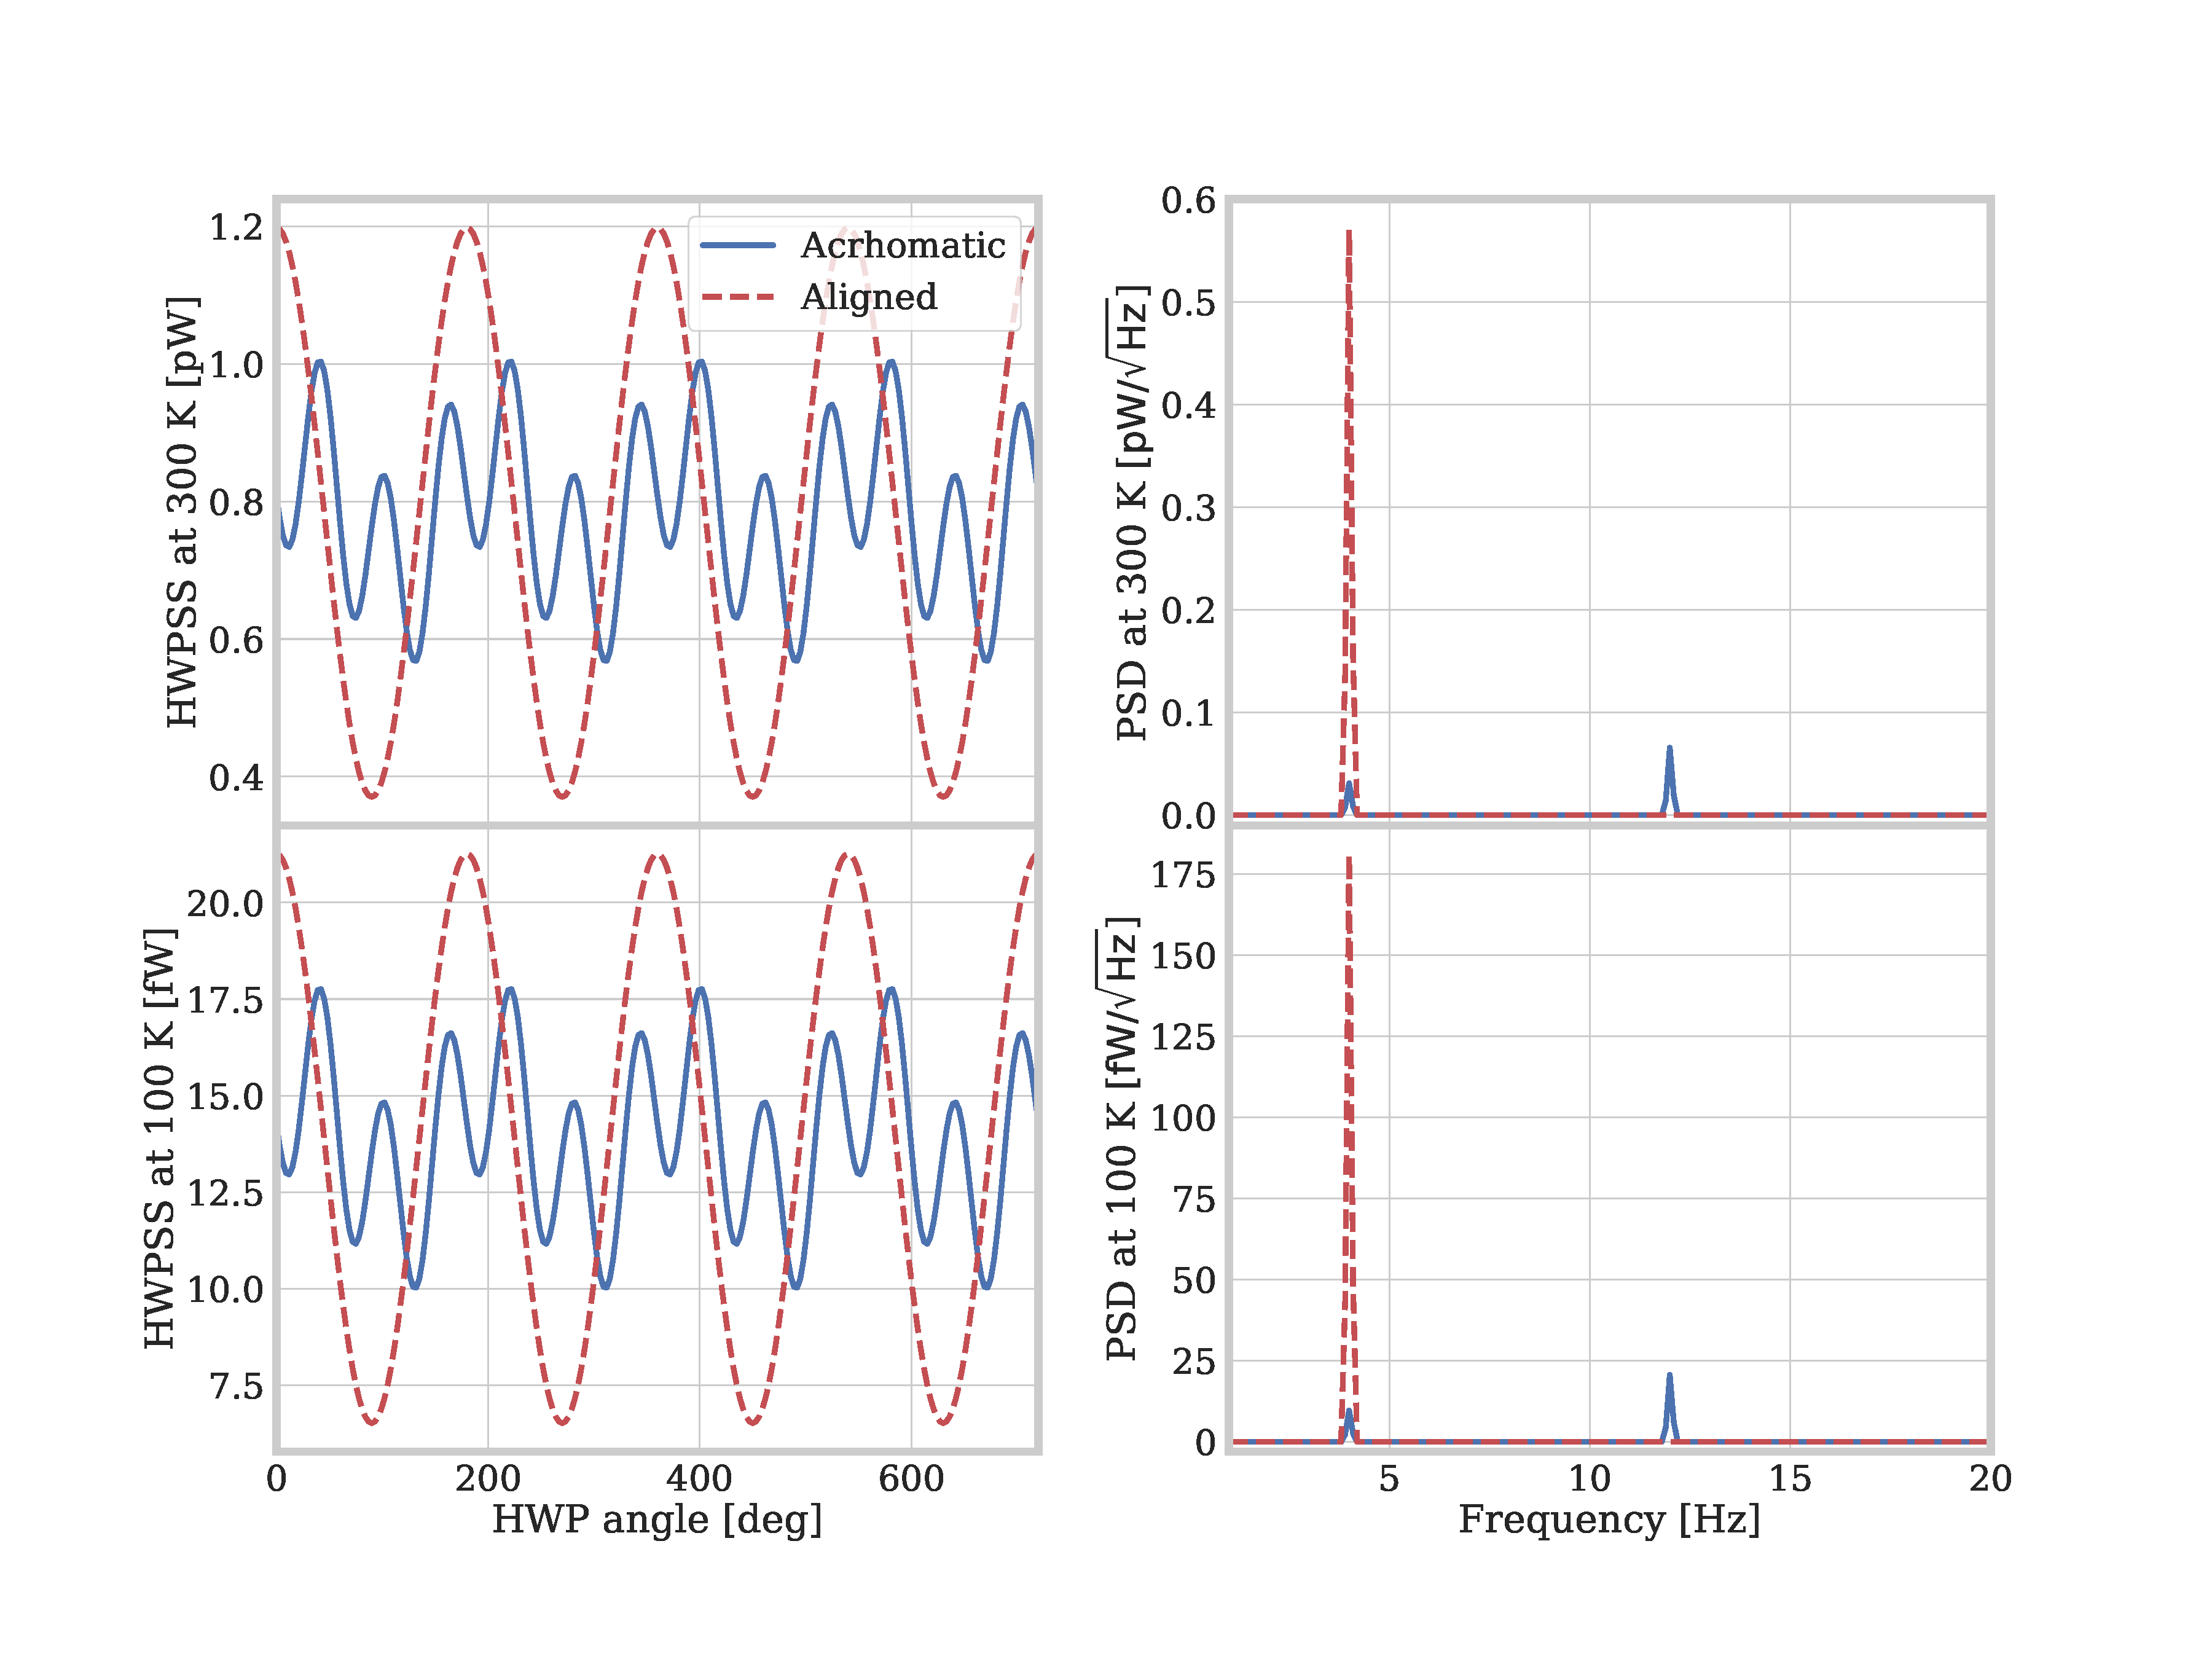
\includegraphics[width=\linewidth, trim=3cm 3cm 4cm 4cm, clip]{PolarizationModulation/Figures/ahwp_thermal_emission_hwpss.pdf}
    \caption{Differential thermal emission from an achromatic HWP, compared to if the three sapphire plate's crystal axes were aligned.}
    \label{fig:ahwp_differential_thermal_emission}
\end{figure}

The first optical mechanism for $4 f_{\mathrm{HWP}}$ HWPSSs is instrumental polarization generated by optics that are sky-side of the HWP. In an idealized telescope, the HWP modulator would be the first optical element, but in many cases, practical limitations, such as a large primary aperture size or the modulator needing to be cryogenically cooled, require the HWP to reside ``behind'' some fraction of the telescope optics. As shown in Figures~\ref{fig:pb2_telescope_cad} and~\ref{fig:so_telescope}, the PB-2b CHWP is located behind the telescope mirrors, vacuum window, and IR filters, while the SO SAT CHWP is similarly located behind the vacuum window and IR filters as well. Because the vacuum windows and IR filters do not have perfect AR coatings and because the SA mirrors are off-axis, there some amount of intensity-to-polarization leakage (I-to-P) generated by differential transmission of the S and P polarizations at non-normal incidence. This I-to-P signal is in turn modulated by the HWP, and its amplitude varies with that of sky intensity. The second optical mechanism for a $4 f_{\mathrm{HWP}}$ signal is that due to non-idealities in the sapphire stack. For example, imperfections or position-dependent thicknesses of the sapphire AR coatings can both generate polarized emission that varies as a function of HWP angle. Such detected $4 f_{\mathrm{HWP}}$ amplitude from such emission will then vary with HWP temperature, contaminating the sky signal. These two examples of optical $4 f_{\mathrm{HWP}}$ are only a subset of possible considerations, and we dig more deeply into other HWPSSs when discussing the hardware requirements of the SA HWPs presented in Chapters~blah and blah.

For a single-stack sapphire HWP, a primary generator of $2 f_{\mathrm{HWP}}$ is differential thermal emission between the ordinary and extraordinary crystal axes. Sapphire's extraordinary axis has both a larger index and a larger loss tangent than those of the ordinary axis, and therefore the two axes have different emissivities. This differential emission rotates with the HWP and shows up at $2 f_{\mathrm{HWP}}$ in the detector data. However, for a three-stack AHWP, the situation is more complicated, as differential emission from sky-side sapphire plates is rotated by detector-side plates. A key question for the AHWP is whether this more complicated has a $4 f_{\mathrm{HWP}}$ component, and if so, how large it is. Figure~blah shows the Mueller-matrix-simulated TOD and power spectral density (PSD) for the AHWP thermal emission, and while there are clear signals at $2 f_{\mathrm{HWP}}$ and $6 f_{\mathrm{HWP}}$, there are no signals at $4 f_{\mathrm{HWP}}$. This particular calculation is done for an ambient temperature AHWP, as thermal emission is the biggest concern for the PB-2a warm waveplate discussed in Chapter~blah.

%%%%%%%%%%%%%%%%%%%%%%%%%%%%%%%%
%%%%%%%%%%%%%%%%%%%%%%%%%%%%%%%%
%%%%%%%%%%%%%%%%%%%%%%%%%%%%%%%%

\section{HWPs for Simons Array}
\label{sec:hwps_for_simons_array}

Now that we have a mathematical framework to describe and assess AHWPs, we move to talk about their implementation within Simons Array (SA). Such a discussion for Simons Observatory, while interesting in its own right, is beyond the scope of this dissertation. Before discussing some SA HWP optical requirements in Section~blah, we first discuss the general philosophy the SA modulator implementation as well as the existing precedent that motivates it.

%%%%%%%%%%%%%%%%%%%%%%%%%%%%%%%%
%%%%%%%%%%%%%%%%%%%%%%%%%%%%%%%%

\subsection{The POLARBEAR HWP}
\label{sec:pb_hwp}

As described in Section~\ref{sec:optical_design}, SA consists of three telescopes with 2.5~m primary mirrors, providing an angular resolution of $\approx$~3~arcmin on the sky, in turn lensing B-mode measurements up to $\ell \sim 2,000$. The SA telescope design is functionally identical to that of its predecessor experiment POLARBEAR, which operated on the Huan Tran Telescope (HTT). Before discussion HWP polarization modulation on PB-1, it is useful to review a few principles of its telescope design, as such details provide a historical context for HWPs in SA.

The HTT's primary and secondary mirrors are in a compact crossed Gregorian configuration, which is designed to optimize telescope mobility and improve low-$\ell$ sensitivity. To understand this phenomenon, recall that atmospheric turbulence evolves with time due to wind, cloud movement, and other weather effects. If the timescale of this atmospheric evolution is shorter than the time it takes to scan across the angular scale of interest, the cosmic signal becomes buried beneath atmospheric fluctuations. In order to beat this atmospheric noise, the sky signal must be modulated on timescales shorter than that of the atmospheric fluctuations, and one way to accomplish this goal is to scan the sky quickly, or equivalently by scanning rapidly in azimuth. When \textit{not} using a HWP, the sky signal appears in side bands around the scan frequency $f_{\mathrm{scan}}$, and therefore, the larger the scan the speed, the smaller the atmospheric 1/f noise.

\begin{figure}
    \centering
    \subfloat[\label{fig:pb1_hwp:a}]{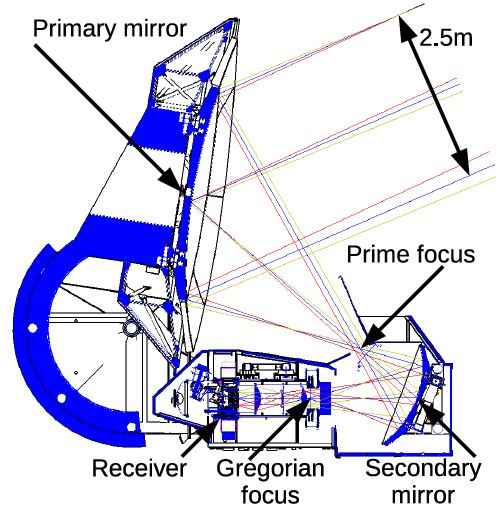
\includegraphics[width=0.5\linewidth, trim=0cm 0cm 0cm 0cm, clip] {PolarizationModulation/Figures/polarbear_telescope.png}}
    \subfloat[\label{fig:pb1_hwp:b}]{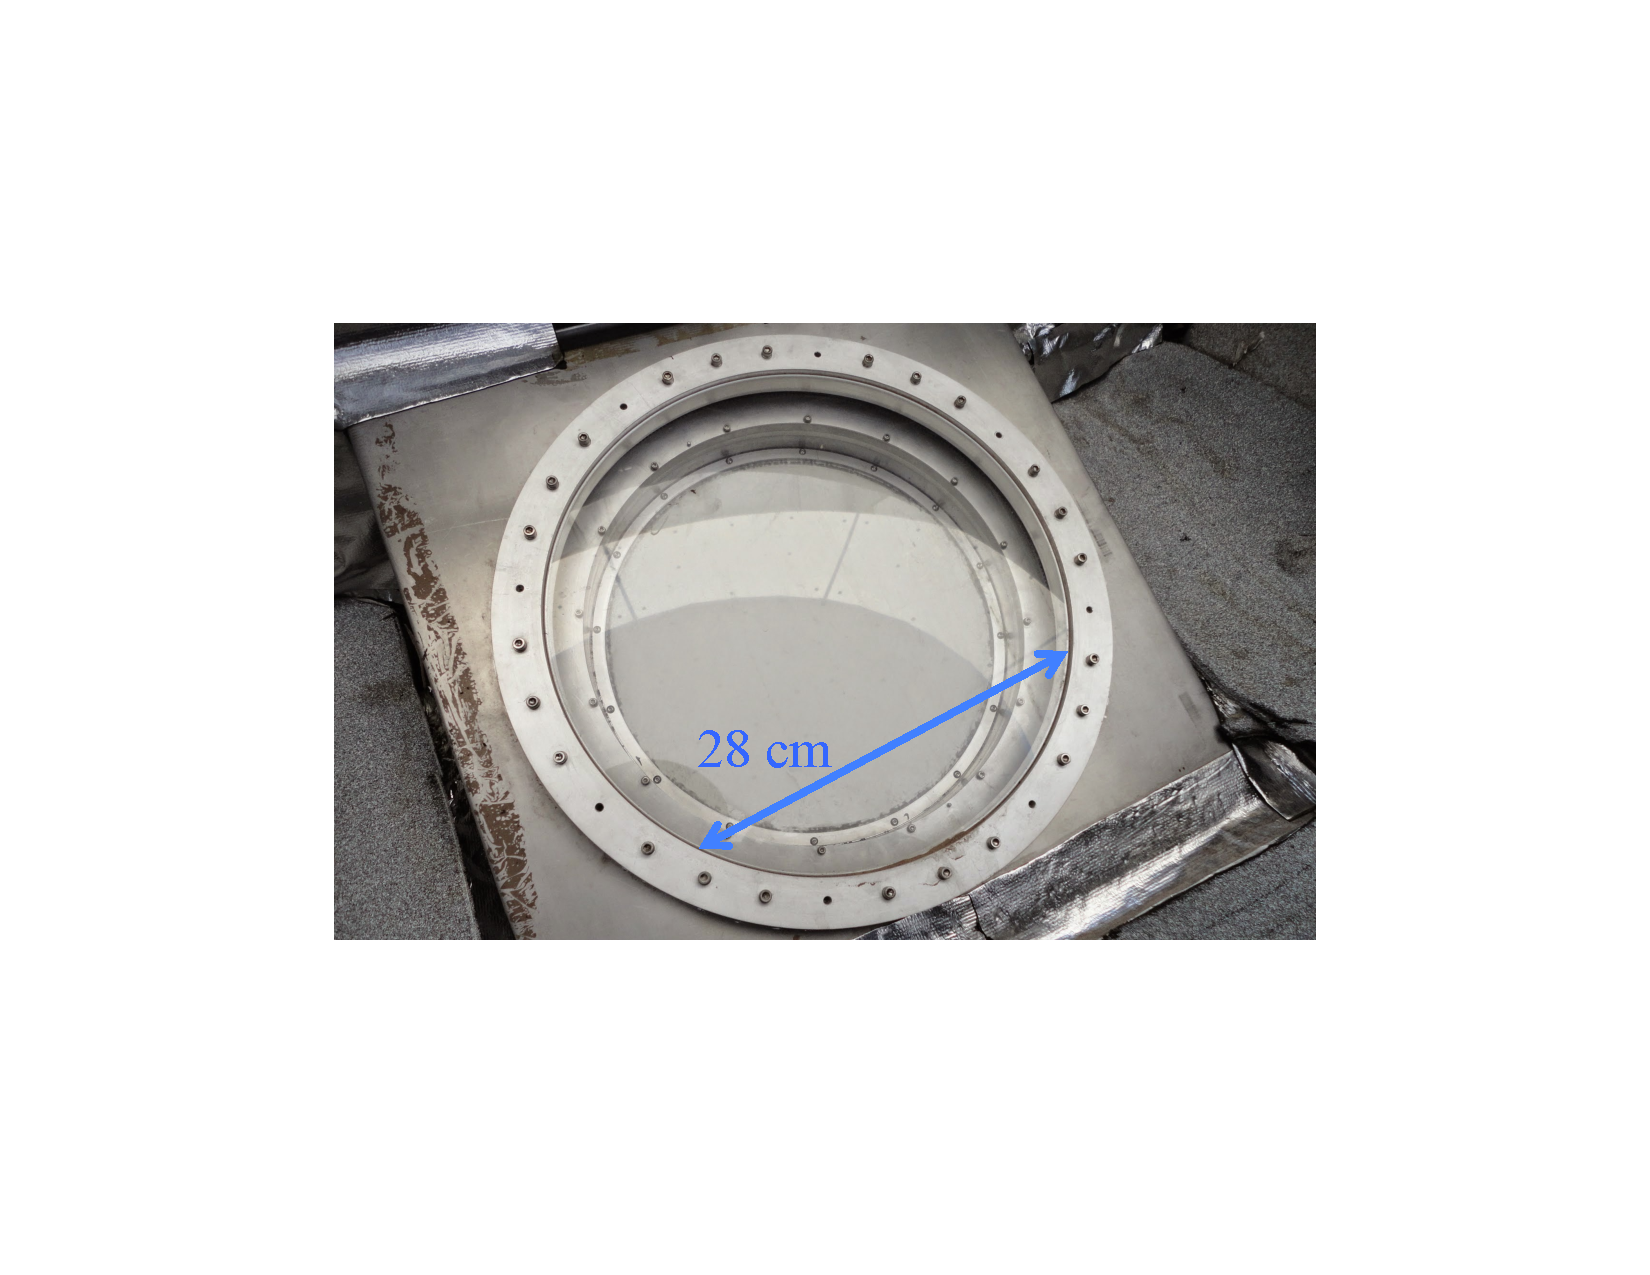
\includegraphics[width=0.5\linewidth, trim=5cm 1.5cm 5cm 5cm, clip]{PolarizationModulation/Figures/PB1_HWP_photo.pdf}}
    \caption{\textbf{Left panel}: A CAD cross section and ray trace of the PB-1 telescope. The PB-1 HWP is located at the prime focus, between the primary and secondary mirrors. Image courtesy of Satoru Takakura's paper. \textbf{Right panel}: A photograph of the PB-1 HWP at prime focus. It is protected from weather by a thin sheet of Muylar, in which the reflection of the primary mirror can be seen. Image courtesy of Satoru Takakura.}
    \label{fig:pb1_telescope_hwp}
\end{figure}

POLARBEAR has Goldilocks-type telescope design, having both a large enough aperture to measure lensing B-modes at $\ell \sim 1,000$ while also being compact enough to scan the sky rapidly, enabling enough large-angular-scale sensitivity to measure primordial B-modes at $\ell \sim 100$. For this reason among others, the initial POLARBEAR telescope design, which observed from 2012-2014, did not use a continuously rotating HWP but instead relied on rapid azimuth motion and effective detector differencing to mitigate 1/f noise in polarization. Such a technique enabled POLARBEAR to make the first polarization-only null-hypothesis rejection of lensing B-modes between $600 < \ell < 3,000$, but pushing to lower $\ell$ proved to be challenging for the reasons described in Sections~\ref{sec:atmospheric_1/f_noise} and~\ref{sec:polarized_beam_systematics}. Therefore, for POLARBEAR's third season of data between 2014-2016, it retroactively installed an ambient-temperature continuously rotating HWP at \important{prime focus} between its primary and secondary mirrors to improve 1/f noise performance.

\begin{figure}
    \centering
    \subfloat[\label{fig:pb1_hwp_performance:a}]{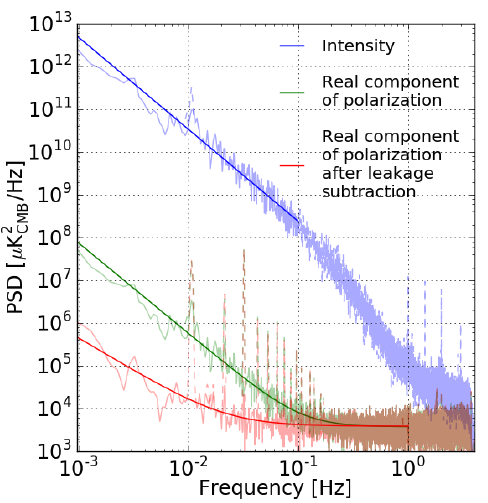
\includegraphics[width=0.5\linewidth, trim=0cm 0cm 0cm 0cm, clip]{PolarizationModulation/Figures/pb1_hwp_noise.png}}
    \subfloat[\label{fig:pb1_hwp_performance:b}]{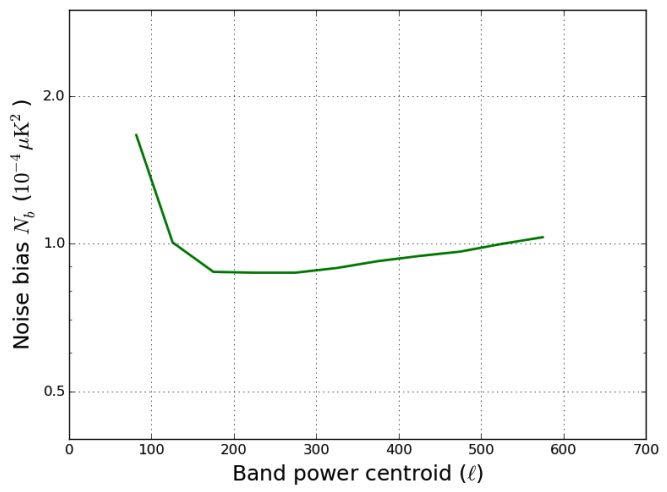
\includegraphics[width=0.5\linewidth, trim=0cm -3cm 0cm 0cm, clip]{PolarizationModulation/Figures/pb1_Nell.png}}
    \caption{Demonstrated performance of the PB-1 HWP. \textbf{Left panel:} PSDs of time streams for coadded detectors cross the full focal plane. An additional I-to-P leakage subtraction is applied to further suppress the 1/f knee in polarization. \textbf{Right panel:} The $N_{\ell}$ curve for the third season of PB-1 data. The achieved $\ell_{\mathrm{knee}} \sim 90$ is a promising demonstration of the HWP's ability to enable low-$\ell$ B-mode science at the Atacama observation site.}
    \label{fig:pb1_hwp_performance}
\end{figure}

POLARBEAR's temporal in both intensity and demodulated polarization, as well as its achieved $N_{\ell}$ spectrum (see Equation~\ref{eq:N_ell_low_frequency_noise}), are shown in Figure~\ref{fig:pb1_hwp_performance}. After an additional I-to-P subtraction associated with detector non-linearity, the PB-1 HWP 1/f noise rejection is quite substantial, enabling white-noise-dominated stability down to frequencies $<$~5~mHz which in turn manifests as an $\ell_{\mathrm{knee}} \sim 90$. This HWP demonstration on PB-1 is central to HWP development within SA. Because the SA optical design is nearly identical to that of PB-1, the success of the POLARBEAR HWP acts a kind of ``existence proof'' that guides the SA HWPs' design and evaluation.


%%%%%%%%%%%%%%%%%%%%%%%%%%%%%%%%
%%%%%%%%%%%%%%%%%%%%%%%%%%%%%%%%

\subsection{The SA HWP}
\label{sec:sa_hwp}

Spurred onward by the successes of the PB-1 HWP, SA has adopted continuously rotating HWPs for their three dichroic telescopes. Before detailing the SA HWP requirements in Section~\ref{sec:sa_hwp_requirements}, it's worth providing a birds-eye view of the the general project structure. When SA was conceived, it was planned to be three POLARBEAR-2-style telescopes, one of which was already in the advanced stages of laboratory evaluation at the KEK High Energy Research Organization in Japan. PB-2 was originally designed to house a three-stack AHWP operating at 4~K near the Lyot stop, but as R\&D advanced, it became clear that a 4~K HWP would not be ready in time for instrument deployment. Therefore, PB-2a, the first installment of SA, opted to move the HWP to ambient temperature, in a similar manner to PB-1. Such a project decision decoupled the PB-2a AHWP development from that of the rest of the receiver, in turn accelerating the overall timeline field operation. However, given their later conception in 2016, PB-2b and PB-2c aimed to move the AHWP back into the cryostat in an effort to suppress photon noise and improve instrument sensitivity. In order to avoid the same problems encountered with PB-2a's 4~K AHWP, the PB-2b/c HWP is located on the 50~K stage, which in turn relaxes several of its mechanical requirements (see Section~\ref{sec:chwp_design_requirements}) and enables its parallel development with the receiver cryostat, just as was so powerful for PB-2a. 

For all three SA receivers, the AHWP was outside of the ``original'' design, and therefore much of the design effort focuses on implementing the modulator effectively without degrading the system's ``heritage'' performance too much. In this way, both in Section~\ref{sec:sa_hwp_requirements} and in Chapters~\ref{ch:pb2a_whwp} through~\ref{ch:chwp_evaluation}, the relevant benchmarks for HWP performance are with respect to the instrument \textit{without} a HWP. Even given this evaluatory approach, we encourage the reader to remember that HWP polarization modulation was always a goal of the POLARBEAR-2 instrument designs. The SA developments also occurred simultaneously with the PB-1 HWP characterization and analysis, and therefore the PB-1 analysis work--in particular that conducted by Satoru Takakura and Neil Goeckner-Wald--play a large role in motivating and framing many of the hardware discussions to follow.

%%%%%%%%%%%%%%%%%%%%%%%%%%%%%%%%
%%%%%%%%%%%%%%%%%%%%%%%%%%%%%%%%
%%%%%%%%%%%%%%%%%%%%%%%%%%%%%%%%

\section{SA HWP requirements}
\label{sec:sa_hwp_requirements}

The content of this dissertation focuses on HWP development for PB-2a and PB-2b, which both observe at 90 and 150~GHz. While we have also worked substantially on the PB-2c HWP, it shares many characteristics with that of PB-2b, and therefore we relegate its detail to future papers led by other authors. In the following section, we discuss the HWP requirements that are common to both the PB-2a and PB-2b HWPs, including sapphire tolerances, rotational velocity, and angle encoder noise.

%%%%%%%%%%%%%%%%%%%%%%%%%%%%%%%%
%%%%%%%%%%%%%%%%%%%%%%%%%%%%%%%%

\subsection{Modulation efficiency}
\label{sec:sa_hwp_requirements_modulation_efficiency}

The first requirement for the SA AHWP is to preserve linear input polarization fraction. As demonstrated in Figure~\ref{fig:poincare_sphere}, an imperfect AHWP converts input linear polarization Q/U into circular polarization V, which is indistinguishable from intensity to a linear polarimeter. Polarized mapping speed (see Equation~\ref{eq:bolocalc_N_ell_mapping_speed_relation}) is related to polarization efficiency as $\mathrm{MS} \propto \varepsilon_{\mathrm{mod}}^{2}$, and therefore it is critically important to maximize polarization efficiency. For SA, we mandate that the AHWP modulation efficiency be $>$~95\%.

\iffalse
\begin{figure}[!t]
    \centering
    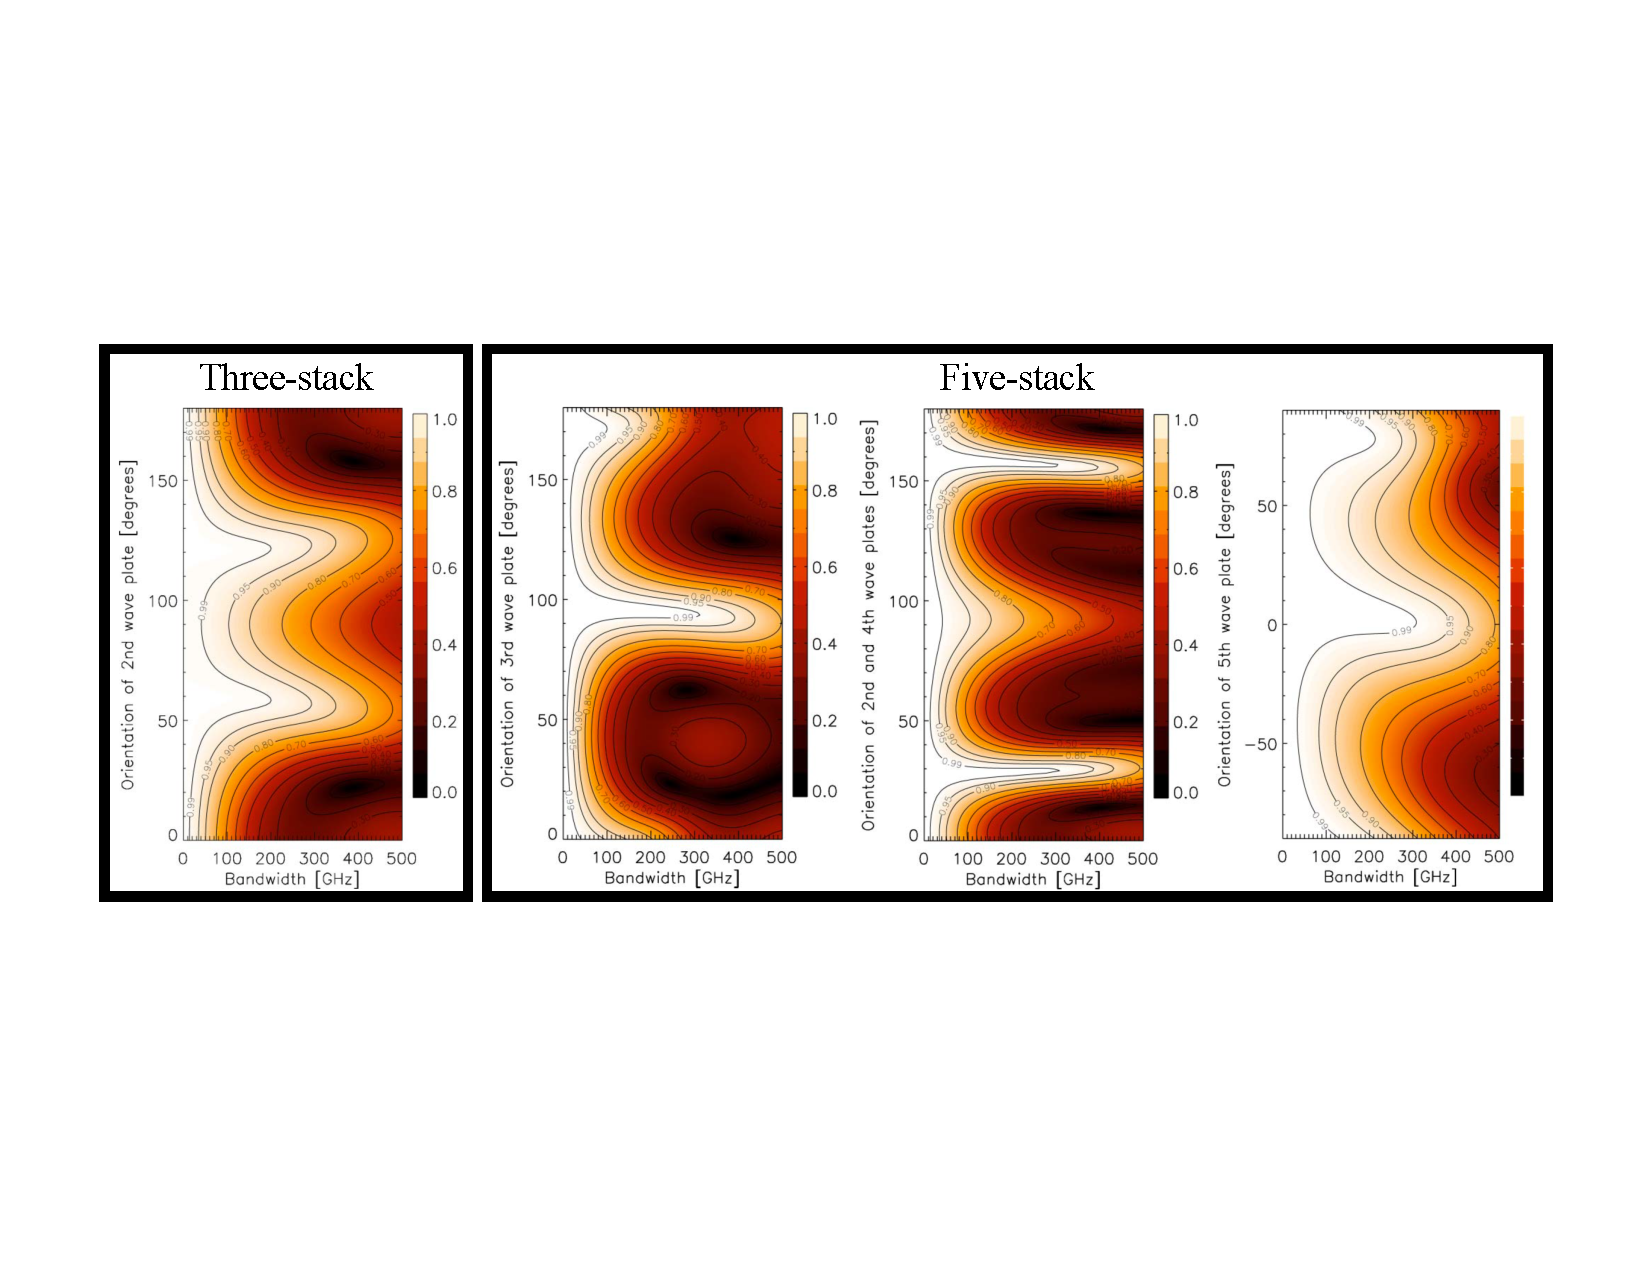
\includegraphics[width=\linewidth, trim=1.2cm 6cm 1.2cm 5.5cm, clip]{PolarizationModulation/Figures/modulation_efficiency_three_five_stack.pdf}
    \caption{Caption}
    \label{fig:modulation_efficiency_three_five_stack}
\end{figure}
\fi

\begin{figure}
    \centering
    \subfloat[\label{fig:modulation_effciency_countors:a}]{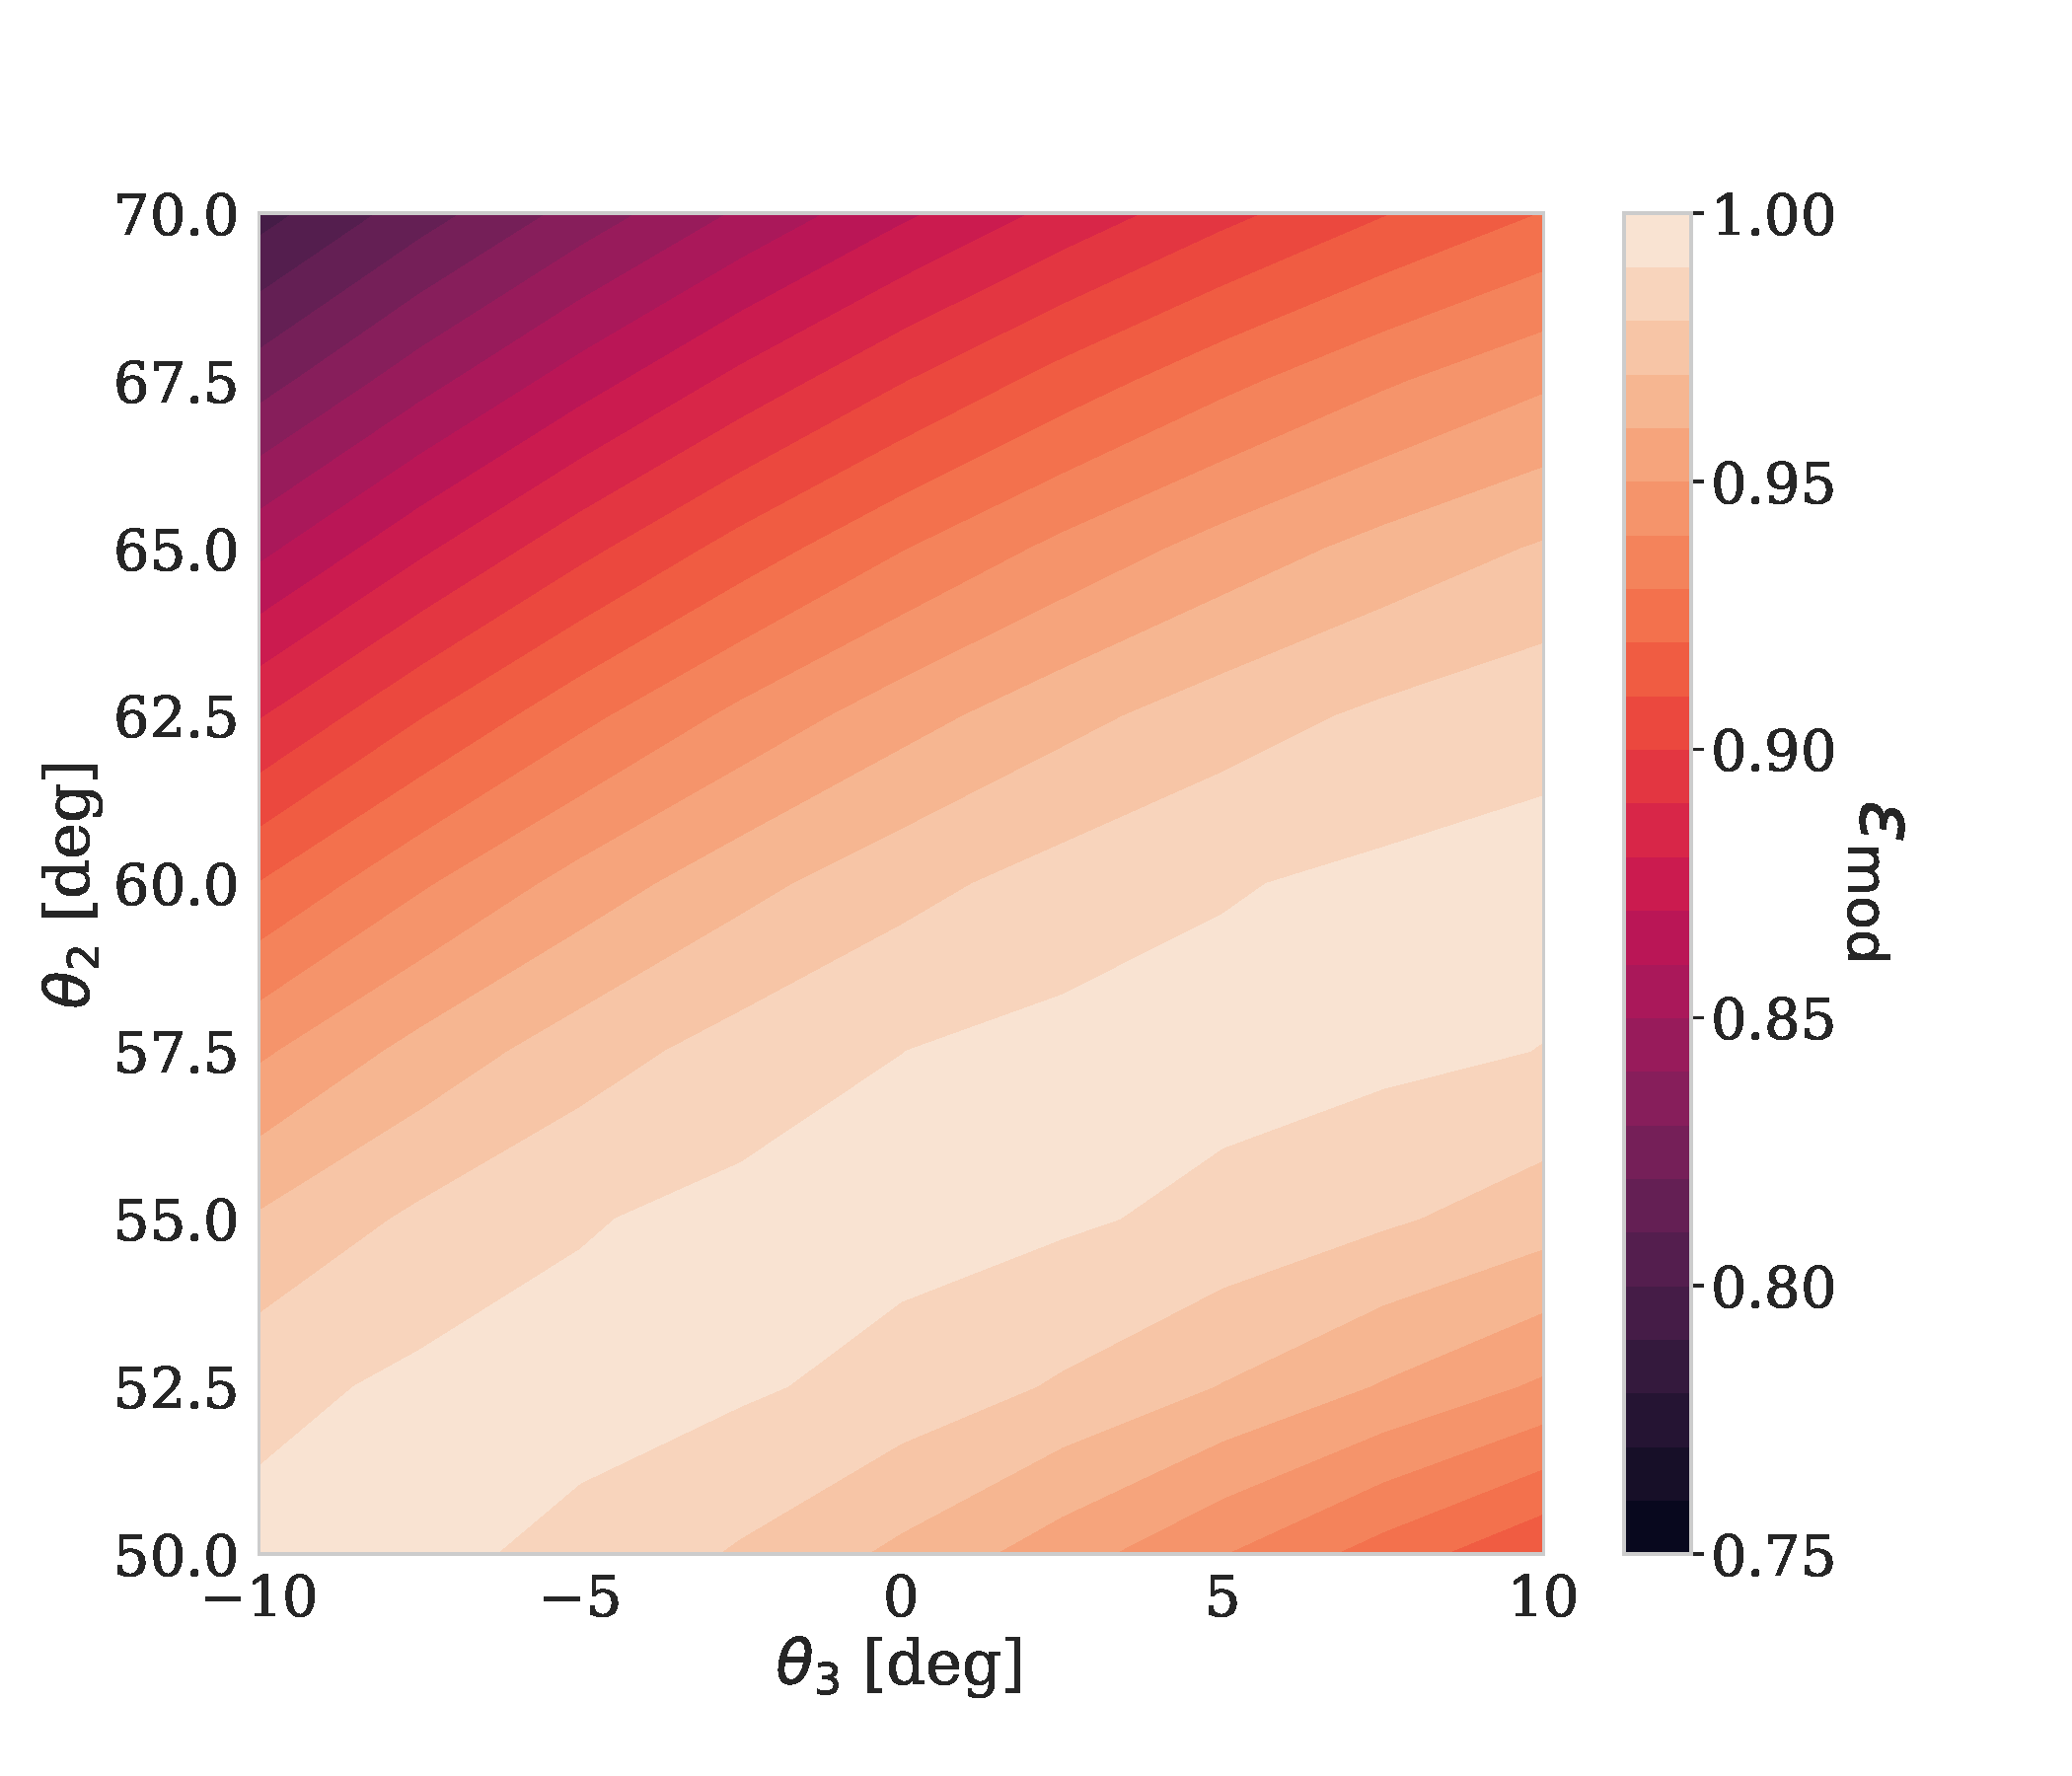
\includegraphics[width=0.5\linewidth, trim=0.7cm 1cm 1.3cm 3cm, clip]{PolarizationModulation/Figures/modulation_efficiency_three_plates_alignment.pdf}}
    \subfloat[\label{fig:modulation_effciency_countors:b}]{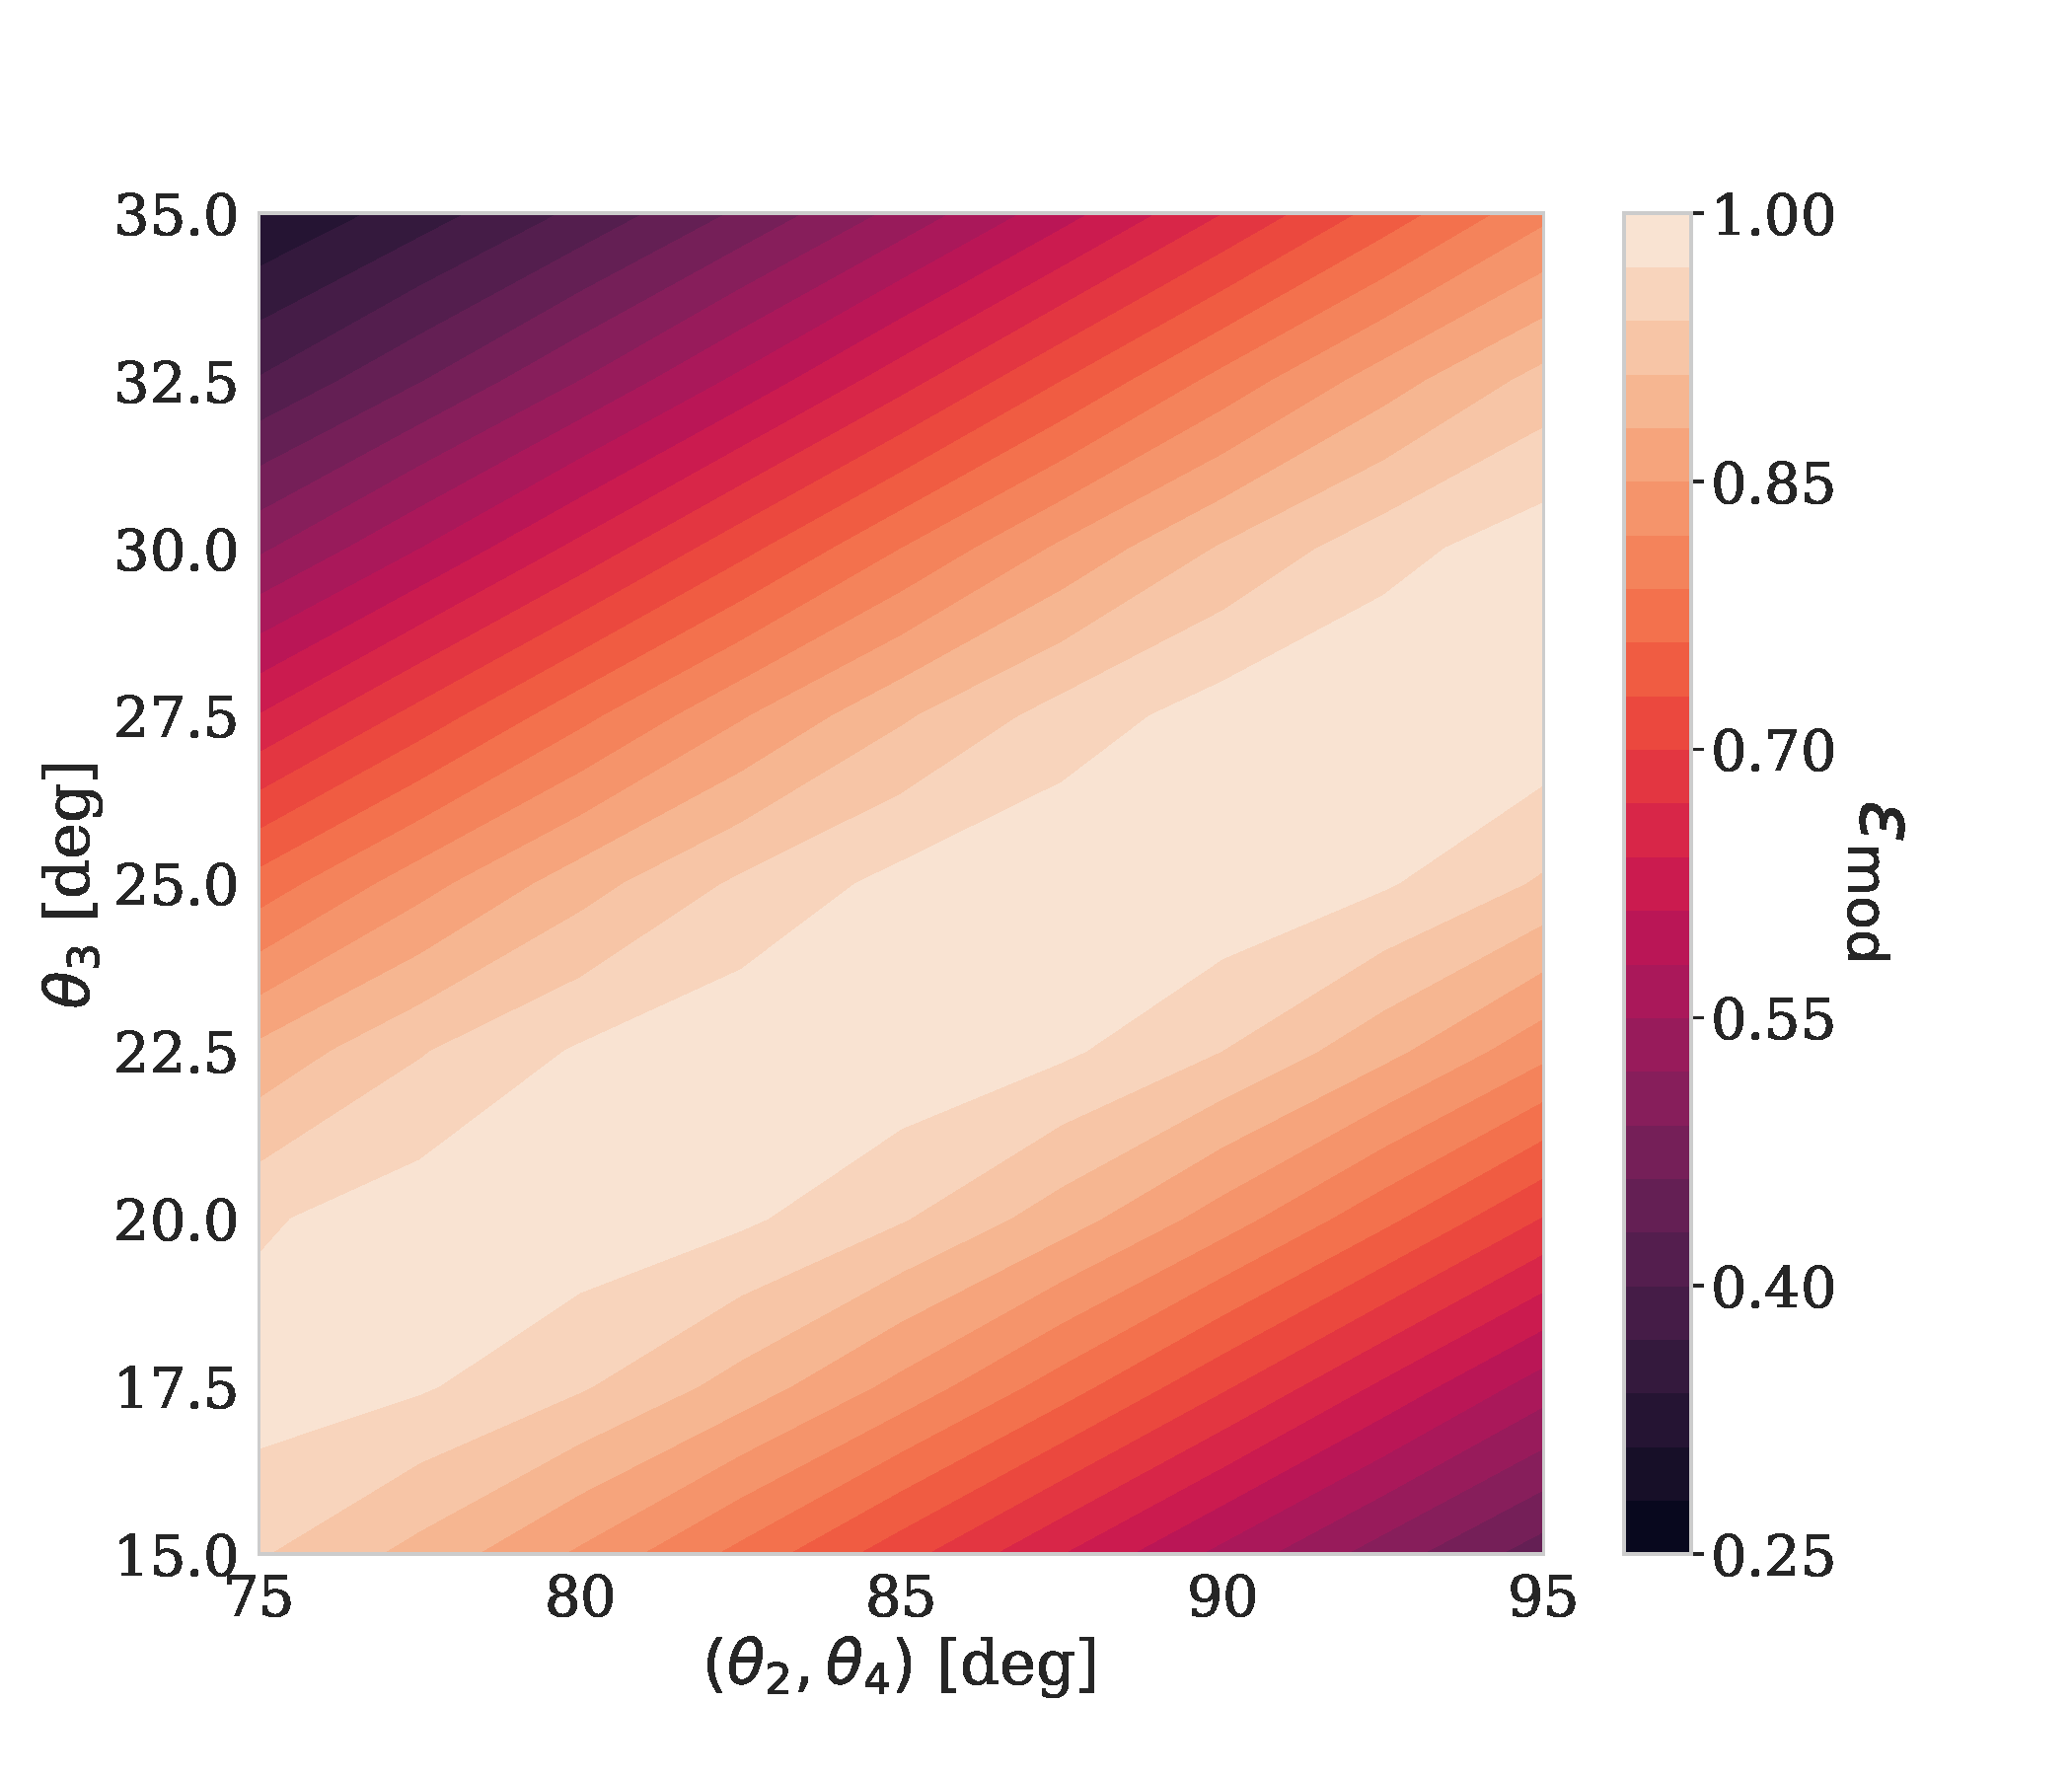
\includegraphics[width=0.5\linewidth, trim=0.7cm 1cm 1.3cm 3cm, clip]{PolarizationModulation/Figures/modulation_efficiency_five_plates_alignment.pdf}}
    \caption{Caption}
    \label{fig:modulation_effciency_countors}
\end{figure}

Modulation efficiency of an AHWP depends on the thickness of its sapphire plates on their relative orientations. The optimization of these parameters for thee- and five-stack AHWPs has been studied in detail by Tomotake Matsumura \textit{et al.}, and the results of that study are shown in Figure~\ref{fig:modulation_efficiency_three_five_stack}. Assuming that the AHWPs are well-enough constructed, a general rule for bandwidth as a function of a number of plates is $\sim [30, 100, 150]$~GHz for a $[1, 3, 5]$-stack HWP. The the total bandwidth for PB-2a/b is $\approx$~110~GHz, and therefore we adopt a 3-stack HWP for both receivers. While it is true that a five-stack strictly does better from the perspective of modulation efficiency, more sapphire windows increased absorptivity, thermal emission, and assembly complexity, all of which have stronger impacts on experiment performance than the $\sim$~1\% mapping speed gains of moving from three plates to five.

Given the three stack design, we can now calculate tolerances on the relative alignment between the plates and on the thickness of the plates. We investigate the impact on modulation by assuming a uniform distribution between the $\pm$ values---as is common practice in manufacturing---and simulating 1,000 Monte Carlo realizations of the resulting band-averaged modulation efficiency in the 90 and 150~GHz bands. The result is shown in Figure~blah, and the resulting thickness and alignment tolerances for PB-2a/b are shown in Table~blah.

%%%%%%%%%%%%%%%%%%%%%%%%%%%%%%%%
%%%%%%%%%%%%%%%%%%%%%%%%%%%%%%%%

\subsection{Rotation velocity}
\label{sec:rotation_velocity}

Another requirement that is common to PB-2a and PB-2b is the HWP's rotational velocity. Recall from Section~\ref{sec:continuous_polarization_modulation} that the polarization modulation frequency $f_{\mathrm{m}}$ is related to the HWP rotation frequency $f_{\mathrm{HWP}}$ as $f_{\mathrm{m}} = 4 f_{\mathrm{HWP}}$. There are two requirements on the modulation frequency that set lower bounds on speed. First, the HWP must rotate fast enough to suppress 1/f noise in the demodulated timestream. In order to do this, the \important{signal side bands} must be in the white-noise dominated temporal regime of the raw data spectrum. The signal side bands $\Delta f_{\mathrm{sig}}$ is the range of frequencies around the \important{carrier frequency} $f_{\mathrm{m}}$ at which the sky signal is modulated. Because faster sky signals appear further from the carrier (see Figure~blah), the \important{modulation bandwidth} is determined by the fastest signal that can be resolved during demodulation.

\begin{figure}
    \centering
    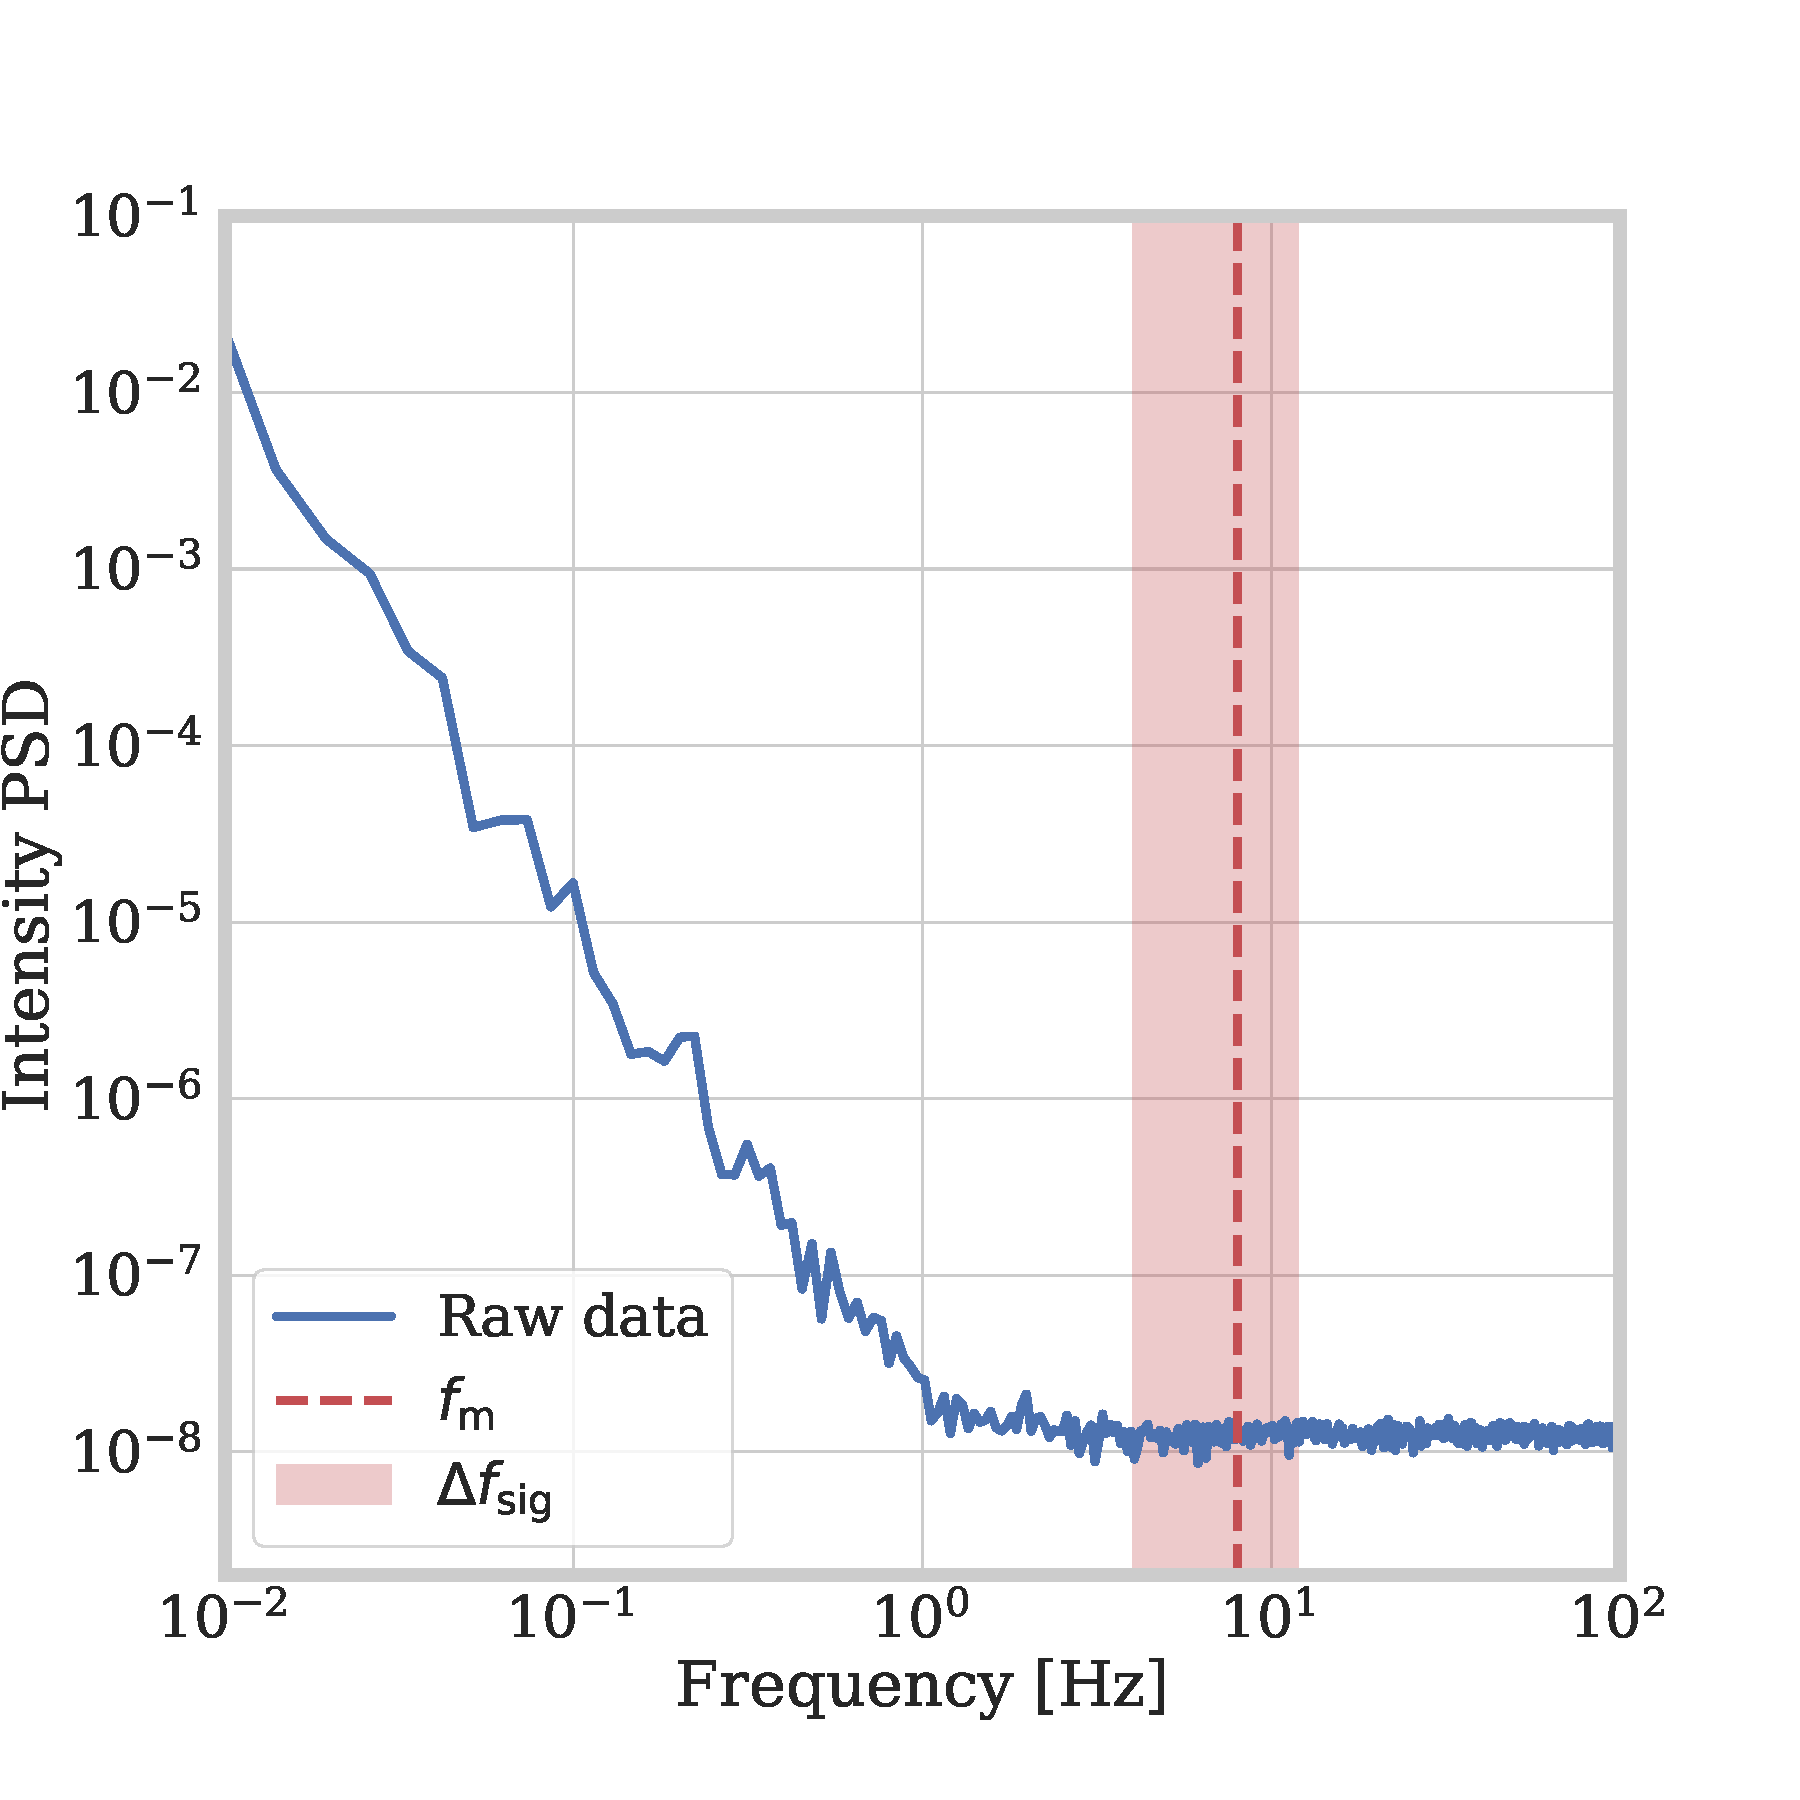
\includegraphics[width=0.5\linewidth, trim=0cm 1cm 1cm 2cm, clip]{PolarizationModulation/Figures/hwp_rotation_frequency.pdf}
    \caption{A notional depiction of HWP modulation band with respect to a dummy-generated, possible raw data PSD, whose 1/f noise is predominantly due to atmospheric fluctuations.}
    \label{fig:hwp_rotation_frequency}
\end{figure}

As discussed in Section~\ref{sec:atmospheric_1/f_noise} and shown in Equation~\ref{eq:scan_speed_to_ell}, the maximum resolvable $\ell_{\mathrm{max}}$ is related to the telescope scan speed as
\begin{equation}
    \ell_{\mathrm{max}} \sim \frac{f_{\mathrm{max}}}{f_{\mathrm{scan}}} \times 180^{\circ} \, .
    \label{eq:maximum_ell_to_modulation_bandwidth}
\end{equation}
As discussed in Section~\ref{sec:optical_design}, PB-2a/b have an angular resolution of $\approx$~3~arcmin at 150~GHz, and if we assume the same telescope scan speed as that used during PB-1's second season of $f_{\mathrm{scan}} = 0.4^{\circ}/\mathrm{sec}$, then the full range of angular scales are resolved within $\Delta f_{\mathrm{sig}} = 2 f_{\mathrm{max}} \approx 4$~Hz of bandwidth. To provide some margin for filtering to higher $\ell$, PB-2a/b reserves 
\begin{equation}
    f_{\mathrm{m}} \pm \Delta f_{\mathrm{sig}} = f_{\mathrm{m}} \pm 4 \; \mathrm{Hz} \, .
\end{equation}
As suggested by the PB-1 intensity PSD shown in Figure~\ref{fig:pb1_hwp_performance}, the atmospheric 1/f knee at the Chile observation site is 1~$\sim$~2~Hz,and therefore we set $f_{\mathrm{m}} \geq 8$~Hz and $f_{\mathrm{HWP}} \geq 2$~Hz, placing the signal band comfortably clear of unpolarized 1/f noise. A depiction of the PB-2 HWP modulation band plotted on top of a dummy intensity PSD is shown in Figure~\ref{fig:hwp_rotation_frequency}.

%%%%%%%%%%%%%%%%%%%%%%%%%%%%%%%%
%%%%%%%%%%%%%%%%%%%%%%%%%%%%%%%%

\subsection{Angle encoding noise}
\label{sec:angle_encoding_noise_requirement}

The final requirement that is common to both the PB-2a and PB-2b HWP systems is the accuracy with which the HWP's rotation angle is reconstructed. An error in the measurement of the rotation angle gives rise an error in the measurement of rotation synchronous signals, which prevents such signals from being fully subtracted during demodulation. 

Both the PB-2a and PB-2b HWPs are located behind the telescope's off-axis mirrors, which induce I-to-P along the $y$ direction (see Fig.~\ref{fig:pb2_ray_trace}). PB-1 measures up to $\approx$~180~$\mathrm{mK_{\mathrm{RJ}}}$ of I-to-P at the prime focus of an SA-style telescope, largely due to emission from the primary reflector.\cite{takakura_performance_2017} Because the PB-2b CHWP is located behind the primary \textit{and} secondary mirrors, we conservatively\footnote{In reality, we expect the I-to-P from the secondary reflector to be less than that of the primary due to its being ellipsoidal with a smaller incident angle. However, the secondary mirror's emission has not been studied in detail, and so we assert that each mirror generates similar I-to-P leakage in order to set a conservative angle jitter requirement.} assert an I-to-P amplitude of
\begin{equation}
    A_{4}^{0} \sim 400 \; \mathrm{mK_{\mathrm{RJ}}} \, ,
    \label{eq:4f_amp}
\end{equation}
where here $\mathrm{K_{RJ}}$ is Rayleigh-Jeans temperature. This mirror polarization is modulated at 4$f_{\mathrm{HWP}}$, and a mismeasurement $\Delta \chi$ of the CHWP angle $\chi$ modifies the 4$f_{\mathrm{HWP}}$ amplitude $A_{4}(\chi)$ as
\begin{eqnarray}
    A_{4}(\chi) & = & A_{4}^{0} \mathrm{cos}(4 \left[ \chi + \Delta \chi \right] ) \nonumber \\ & \approx & A_{4}^{0} \mathrm{cos}(4 \chi) - 4 \, A_{4}^{0} \mathrm{sin}(4 \chi) \Delta \chi \, ,
    \label{eq:freq_mod}
\end{eqnarray}
\noindent
such that
\begin{equation}
    \Delta A_{4} = -4 \, A_{4}^{0} \mathrm{sin}(4 \chi) \Delta \chi \, .
    \label{eq:delta_chi}
\end{equation}
Assuming that the angle jitter is random, its average effect on the detected noise spectrum is
\begin{equation}
    \mathrm{NET_{CMB}^{HWP}} = 2 \sqrt{2} \,  \frac{\mathrm{d} T_{\mathrm{CMB}}}{\mathrm{d} T_{\mathrm{RJ}}} \, A_{4}^{0} \, \sigma_{\chi} \, ,
    \label{eq:encoder_noise}
\end{equation}
\noindent
where $\sigma_{\chi}$ is the root mean square (RMS) of $\Delta \chi$, $\mathrm{NET_{CMB}^{HWP}}$ is the noise equivalent CMB temperature (see Equation~\ref{eq:net}) of the angle jitter, and $\mathrm{d} T_{\mathrm{CMB}} / \mathrm{d} T_{\mathrm{RJ}} = 1.7$ is evaluated at 150~GHz. 

All detectors on the focal plane are demodulated using the same angle encoder data, and therefore any noise in the encoder reconstruction is common to all detectors. Therefore, in order for angle encoder noise to not significantly contribute to the noise of the detector array, $\mathrm{NET_{CMB}^{HWP}}$ needs to be subdominant to the \textit{array NET}, which is forecasted to be $\mathrm{NET_{CMB}^{arr}} = 5.8 \mathrm{\mu K / \sqrt{Hz}}$ for both PB-2a and PB-2b. Given this constraint, the angle noise requirement for the SA HWPs is
\begin{equation}
    \sigma_{\chi} \ll 3 \, \mathrm{\mu rad / \sqrt{Hz}} \, .
\end{equation}
This requirement drives several aspects of the HWP designs, including excellent rotation stability, low encoder noise, and sufficient encoder resolution.

%%%%%%%%%%%%%%%%%%%%%%%%%%%%%%%%
%%%%%%%%%%%%%%%%%%%%%%%%%%%%%%%%

\subsection{Temperature stability}
\label{sec:sa_hwp_requirement_temperature_stability}

%%%%%%%%%%%%%%%%%%%%%%%%%%%%%%%%
%%%%%%%%%%%%%%%%%%%%%%%%%%%%%%%%

\subsection{Vibration}
\label{sec:sa_hwp_requirement_temperature_stability}

